
\documentclass{scrartcl}
% alternative article or report


%%%%% PACKAGES

% small tweaks and nicer typography
\usepackage{microtype}
\usepackage{hyperref}

% changes language to German
% gives proper date, and correct hyphenation
\usepackage[ngerman]{babel}

%\usepackage[fixlanguage]{babelbib}
%\selectbiblanguage{german}

% dealing with figures
\usepackage[figurename=Abb.]{caption}
\usepackage{subcaption}
\usepackage{wrapfig}

% basic math stuff
\usepackage{mathtools}
\usepackage{amssymb}
\usepackage{amsthm}
%\usepackage{tikz-cd}
\usepackage{cancel}

% tikz
\usepackage{tikz}
\usetikzlibrary{positioning}
%\usetikzlibrary{patterns}
\usetikzlibrary{babel}
\tikzset{>=stealth}

\newcommand{\tikzmark}[3][]{\tikz[remember picture,baseline] \node [anchor=base,#1](#2) {$#3$};}

\usepackage{booktabs}
\usepackage{bm}
%\usepackage{minted}

% for inkscape images
%\usepackage{pdftricks}
%\begin{psinputs}
%   \usepackage{pstricks}
%   \usepackage{multido}
%\end{psinputs}
%\usepackage[pdf]{pstricks}
%\usepackage{import}
%\import{../Resources}{ErweiterungNullrand.pdf_tex}

% title page
\usepackage{BA_Titelseite}

%%%%% CONFIGURATION

% prevents automatic line breaks inside of equations
% since it looks bad
\binoppenalty = \maxdimen
\relpenalty   = \maxdimen

% theorem-like environments
\newcounter{everything}
\newtheorem{corollary}[everything]{Korollar}
\newtheorem{lemma}[everything]{Lemma}
\newtheorem{proposition}[everything]{Proposition}
\newtheorem{theorem}[everything]{Satz}


%%%%% CUSTOM COMMANDS

% real numbers via \R
% complex numbers via \C
% general field via \K
\def\C{\mathbb{C}}
\def\R{\mathbb{R}}
\def\K{\mathbb{K}}
\def\Q{\mathbb{Q}}
\def\Z{\mathbb{Z}}
\def\N{\mathbb{N}}
\def\H{\mathbb{H}}
\def\e{\varepsilon}
\def\ev{e}

\newcommand{\cA}{\mathcal{A}}
\newcommand{\cB}{\mathcal{B}}
\newcommand{\cC}{\mathcal{C}}
\newcommand{\cD}{\mathcal{D}}
\newcommand{\cE}{\mathcal{E}}
\newcommand{\cF}{\mathcal{F}}
\newcommand{\cG}{\mathcal{G}}
\newcommand{\cH}{\mathcal{H}}
\newcommand{\cI}{\mathcal{I}}
\newcommand{\cJ}{\mathcal{J}}
\newcommand{\cK}{\mathcal{K}}
\newcommand{\cL}{\mathcal{L}}
\newcommand{\cM}{\mathcal{M}}
\newcommand{\cN}{\mathcal{N}}
\newcommand{\cO}{\mathcal{O}}
\newcommand{\cP}{\mathcal{P}}
\newcommand{\cQ}{\mathcal{Q}}
\newcommand{\cR}{\mathcal{R}}
\newcommand{\cS}{\mathcal{S}}
\newcommand{\cT}{\mathcal{T}}
\newcommand{\cU}{\mathcal{U}}
\newcommand{\cV}{\mathcal{V}}
\newcommand{\cW}{\mathcal{W}}
\newcommand{\cX}{\mathcal{X}}
\newcommand{\cY}{\mathcal{Y}}
\newcommand{\cZ}{\mathcal{Z}}

\newcommand{\bA}{\mathbb{A}}
\newcommand{\bB}{\mathbb{B}}
\newcommand{\bC}{\mathbb{C}}
\newcommand{\bD}{\mathbb{D}}
\newcommand{\bE}{\mathbb{E}}
\newcommand{\bF}{\mathbb{F}}
\newcommand{\bG}{\mathbb{G}}
\newcommand{\bH}{\mathbb{H}}
\newcommand{\bI}{\mathbb{I}}
\newcommand{\bJ}{\mathbb{J}}
\newcommand{\bK}{\mathbb{K}}
\newcommand{\bL}{\mathbb{L}}
\newcommand{\bM}{\mathbb{M}}
\newcommand{\bN}{\mathbb{N}}
\newcommand{\bO}{\mathbb{O}}
\newcommand{\bP}{\mathbb{P}}
\newcommand{\bQ}{\mathbb{Q}}
\newcommand{\bR}{\mathbb{R}}
\newcommand{\bS}{\mathbb{S}}
\newcommand{\bT}{\mathbb{T}}
\newcommand{\bU}{\mathbb{U}}
\newcommand{\bV}{\mathbb{V}}
\newcommand{\bW}{\mathbb{W}}
\newcommand{\bX}{\mathbb{X}}
\newcommand{\bY}{\mathbb{Y}}
\newcommand{\bZ}{\mathbb{Z}}

\newcommand{\hu}{\hat{u}}
\newcommand{\hv}{\hat{v}}
\newcommand{\hA}{\hat{A}}
\newcommand{\hC}{\hat{C}}
\newcommand{\hR}{\hat{R}}
\newcommand{\hb}{\hat{b}}
\newcommand{\hw}{\hat{w}}
\newcommand{\hW}{\hat{W}}
\newcommand{\hM}{\hat{M}}
\newcommand{\hV}{\hat{V}}
\newcommand{\hQ}{\hat{Q}}
\newcommand{\hq}{\hat{q}}
\newcommand{\hp}{\hat{p}}
\newcommand{\hl}{\hat{\ell}}

\newcommand{\tiS}{\tilde{S}}
\newcommand{\tiu}{\tilde{u}}
\newcommand{\tih}{\tilde{h}}
\newcommand{\tie}{\tilde{\varepsilon}}
\newcommand{\tiE}{\tilde{E}}
\newcommand{\tiomega}{\tilde{\omega}}
\newcommand{\tiOmega}{\tilde{\Omega}}
\newcommand{\tir}{\tilde{r}}
\newcommand{\tiB}{\tilde{B}}
\newcommand{\tiA}{\tilde{A}}
\newcommand{\tisigma}{\tilde{\sigma}}

\newcommand{\erw}{\mathfrak{E}}			% Erweiterung

\newcommand{\dif}[1]{\,\mathrm{d} #1}
%\newcommand{\norm}[1]{\lVert #1 \rVert}
%\newcommand{\abs}[1]{\left| #1 \right|}
\newcommand{\bnorm}[1]{\left\lVert #1\right\rVert}
\newcommand{\vii}[2]{\ensuremath{\begin{bmatrix}#1 \\ #2 \end{bmatrix}}}
\newcommand{\mii}[4]{\ensuremath{\begin{bmatrix}#1&#2 \\ #3&#4 \end{bmatrix}}}
\newcommand{\mc}[1]{\mathcal{#1}}


%%%%%%%%%%    Math operators    %%%%%%%%%%%%%%%%%%%%%%%%%%%

\DeclareMathOperator{\Id}{Id}             % identity morphism
% \DeclareMathOperator{\ker}{ker}           % kernel
\DeclareMathOperator{\rg}{rg}             % image
\DeclareMathOperator{\defekt}{def}             % defect
\DeclareMathOperator{\im}{im}             % image
\DeclareMathOperator{\Hom}{Hom}           % homomorphisms
\DeclareMathOperator{\End}{End}           % endomorphisms
\DeclareMathOperator{\Span}{Span}         % linear span
\DeclareMathOperator{\grad}{\nabla}         % gradient
\DeclareMathOperator{\diam}{diam}         % gradient
\DeclareMathOperator{\Tr}{Tr}       	  % trace
\DeclareMathOperator{\diver}{Div}			% divergence
\DeclareMathOperator{\supp}{supp}			% support
\DeclareMathOperator{\dist}{dist}			% distance
\DeclareMathOperator{\inter}{int}			% interiour
\DeclareMathOperator{\epi}{epi}			% epigraph
\DeclareMathOperator{\hyp}{hyp}			% hypograph
\DeclareMathOperator{\Lip}{Lip}			% lipschitz konstant
\DeclareMathOperator{\graph}{graph}			% graph

% inner product (scalar product) via \inner{v, w}
% norm via \norm{x}
% absolute value via \abs{x}
% use the star-version for automatic scaling
\DeclarePairedDelimiter{\abs}{\lvert}{\rvert}
\DeclarePairedDelimiter{\inner}{\langle}{\rangle}
\DeclarePairedDelimiter{\norm}{\lVert}{\rVert}

% \vect{ x // y // z } for a column vector with entries x, y, z
% similarly for larger vectors
% in this code:  1 = number of arguments
%               #1 = first argument
\newcommand{\vect}[1]{\begin{bmatrix} #1 \end{bmatrix}}


% \conj{z} for complex conjugation
\newcommand{\conj}{\overline}

%%%%%%% GENERAL STYLE %%%%%%%%%%%%%%%%%%

\setcounter{tocdepth}{3}


%%%%% TITLE PAGE %%%%%%%%%%%%%%%%%%%%%%%%%%

%Namen des Verfassers der Arbeit
\author{Theo Koppenhöfer}
%Geburtsdatum des Verfassers
\geburtsdatum{9. November 2000}
%Gebortsort des Verfassers
\geburtsort{Heidelberg}
%Datum der Abgabe der Arbeit
\date{27.\ Juli 2022}

%Name des Betreuers
% z.B.: Prof. Dr. Peter Koepke
\betreuer{Betreuer: Prof. Dr. Joscha Gedicke}
%Name des Zweitgutachters
\zweitgutachter{Zweitgutachter: Prof. Dr. Jochen Garcke}
%Name des Instituts an dem der Betreuer der Arbeit tätig ist.
%z.B.: Mathematisches Institut
%\institut{Mathematisches Institut}
%\institut{Institut f\"ur Angewandte Mathematik}
\institut{Institut f\"ur Numerische Simulation}
%\institut{Forschungsinstitut f\"ur Diskrete Mathematik}
%Titel der Bachelorarbeit
\title{Adaptive Finite Elemente für Lineare Elastizität}
%Do not change!
\ausarbeitungstyp{Bachelorarbeit Mathematik}


%%%%% The content starts here %%%%%%%%%%%%%


\begin{document}

\maketitle

\tableofcontents

% hide page numbering for this page
\thispagestyle{empty}

\newpage

\setcounter{page}{1}

\addcontentsline{toc}{section}{\protect\numberline{}Zusammenfassung}
\section*{Zusammenfassung}

Viele Probleme aus der Statik werden mit Finite-Elemente-Methoden gelöst. Hierbei ist die Wahl des Gitters für den Fehler der Lösung oft entscheidend, weshalb a posteriori Fehlerschätzer eingesetzt werden, um das Gitter adaptiv zu verfeinern. In dieser Bachelor\-arbeit wird ein residualer a posteriori Fehlerschätzer für Probleme in der linearen Elastizität konstruiert und gezeigt, dass dieser zuverlässig und lokal effizient ist. Dazu werden grundlegende Begriffe aus der linearen Elastizität definiert, eine variationelle Formulierung hergeleitet und mithilfe der Kornschen Ungleichung und des Lax-Milgram-Lemmas Existenz und Eindeutigkeit gezeigt. Es wird ein P1 Finites Element besprochen und implementiert. Anschließend werden in numerischen Experimenten die Effizienz und Zuverlässigkeit des Schätzers bestätigt. Hierbei sieht man auch das Locking-Phänomen und die lineare Konvergenz für das P1 Finite Element.


\section{Einleitung}

\begin{wrapfigure}{r}{0.46\textwidth}
\centering
\vspace*{-1.3cm}
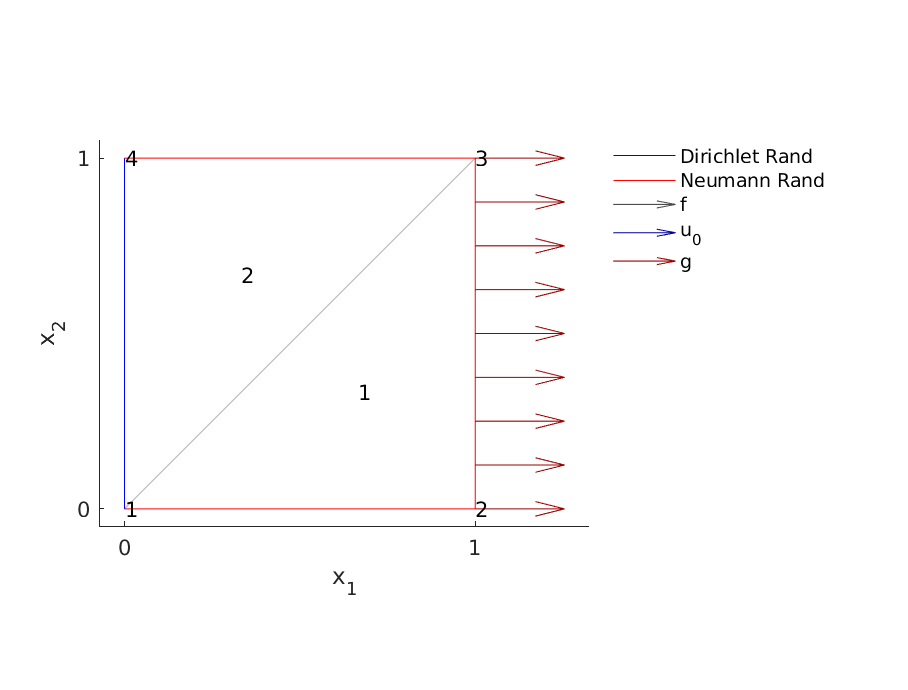
\includegraphics[width=0.46\textwidth]{Plots/PullBoxInitial2}
\vspace*{-1.2cm}
\caption{Anfangsbedingungen}
\label{pl:PullBoxInitial}
\end{wrapfigure}

Man stelle sich folgendes Problem vor: Ein quadratförmiges Werkstück wird an der linken Kante festgehalten und es wird an der rechten Kante gezogen, wie in Abbildung \ref{pl:PullBoxInitial} dargestellt. Gesucht ist die Verformung des Werk\-stücks.
Dies ist ein typisches Problem der Statik. Allerdings ist schon dieses simple Beispiel praktisch nur noch numerisch und nicht mehr analytisch lösbar. Für die numerische Lösung werden oft Finite-Elemente-Methoden verwendet. Hierbei wird das Ausgangsobjekt mit einem Gitter in viele kleinere Teilgebiete, Elemente genannt, unterteilt. Anschließend wird für das Gitter eine Lösung des Problems berechnet. Eine solche Lösung ist für dieses Problem in Abbildung \ref{pl:PullBoxUniformSoln} dargestellt. Allerdings hängt der Fehler der berechnete Lösung von der Wahl des Gitters ab. Idealerweise wollen wir das Gitter an den Stellen stärker verfeinern, wo die Lösung besonders ungenau ist. Dafür benötigt man eine Methode, den Fehler der berechneten Lösung abzuschätzen ohne die exakte Lösung zu kennen. Dies führt auf den Begriff des a posteriori Fehlerschätzers. Man verwendet einen solchen Fehlerschätzer, um das Gitter adaptiv zu verfeinern, was für unser Problem in Abbildung \ref{pl:PullBoxAdaptiveSoln} dargestellt ist.

\begin{figure}[h]
\centering
\begin{minipage}{0.475\textwidth}
\centering
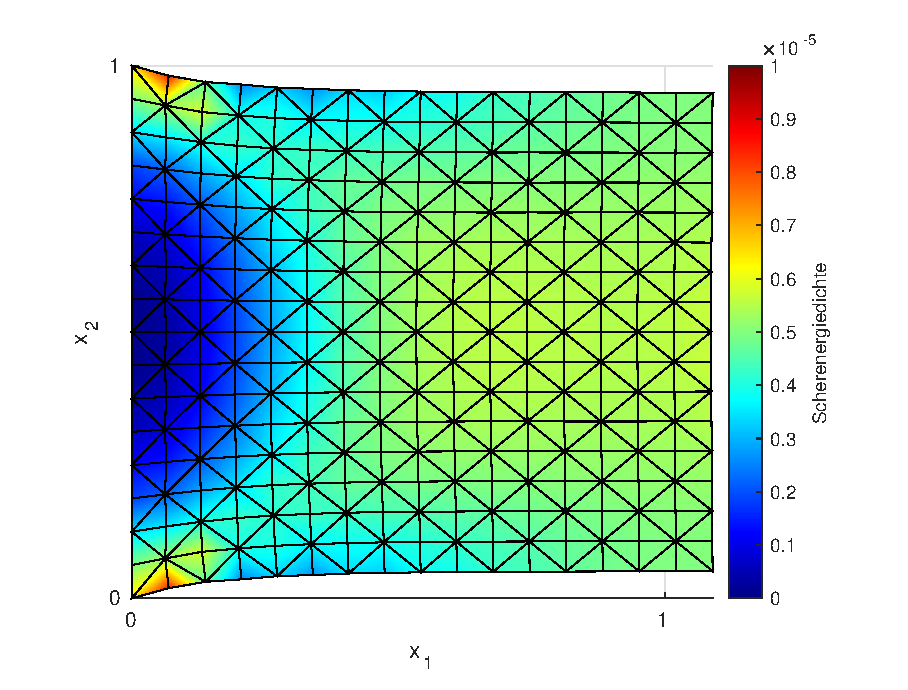
\includegraphics[width=0.9\textwidth]{Plots/PullBoxUniformDeform3}
\caption{uniforme Gitterverfeinerung}
\label{pl:PullBoxUniformSoln}
\end{minipage}
\hfill
\begin{minipage}{0.475\textwidth}
\centering
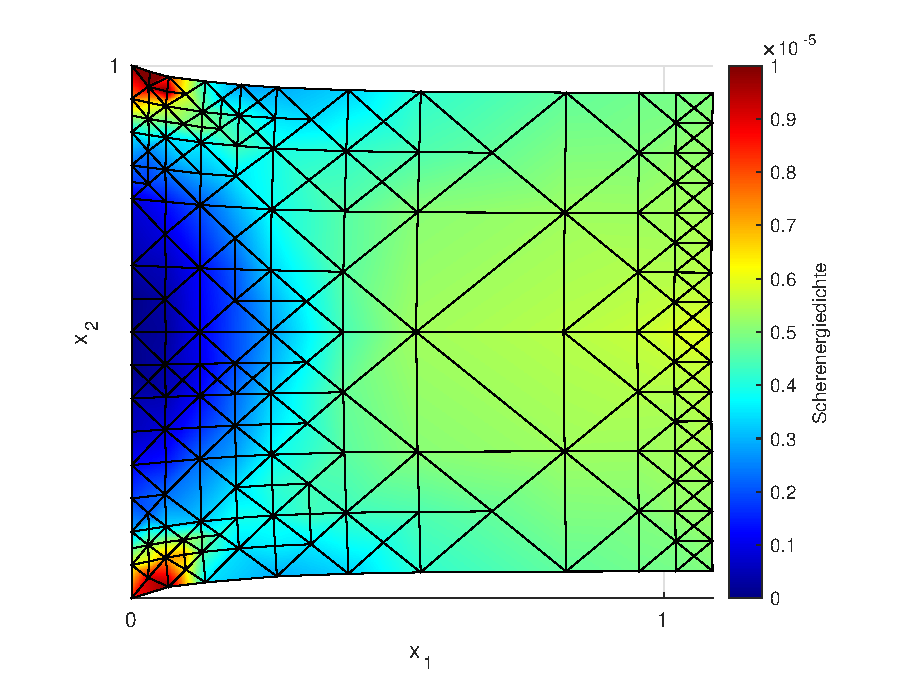
\includegraphics[width=0.9\textwidth]{Plots/PullBoxAdaptiveDeform3}
\caption{adaptive Gitterverfeinerung}
\label{pl:PullBoxAdaptiveSoln}
\end{minipage}
\end{figure}

Diese Arbeit soll einen kurzen Einblick in den Bereich der linearen Elastizitätstheorie liefern und einen residualen Fehlerschätzer für die adaptive Gitterverfeinerung konstruieren. Anschließend soll der Fehlerschätzer in numerischen Experimenten getestet werden.

Dazu werden im nachfolgenden Kapitel grundlegende Begriffe der linearen Elastizität eingeführt und mehrere Formulierungen des Problems motiviert. Das Kapitel beginnt mit der Definition der Begriffe "`Verschiebung"' und "`Spannungstensor"' und bespricht dann die Randbedingungen des Problems. Das Problem wird als Kräftegleichgewicht formuliert und daraus wird dann eine differenzielle Formulierung hergeleitet. Es folgt ein Intermezzo zu den Materialgesetzen, wobei wir uns im Wesentlichen auf lineare isotrope Materialien beschränken. Danach wird aus der differenziellen Formulierung eine variationelle Formulierung mit dem Prinzip der virtuellen Arbeit hergeleitet. Anschließend wird ein Ausdruck für die Energie hergeleitet, was eine Formulierung als Optimierungsproblem erlaubt, die äquivalent zur variationellen Formulierung ist.

Es folgt ein Kapitel über Existenz und Eindeutigkeit der schwachen Formulierungen. Hierfür nutzen wir das Lax-Milgram Lemma, was unter Anderem die Elliptizität der Bilinearform $a$ voraussetzt. Die Elliptizität von $a$ folgt im Wesentlichen aus den Kornschen Ungleichungen. Dazu wird zunächst die Kornsche Ungleichung ohne Randbedingungen auf dem Ganzraum gezeigt. Es wird dann ein Erweiterungsoperator von Epigraphen stetig differenzierbarer Funktionen auf den Ganzraum konstruiert. Dieser liefert zusammen mit einer Zerlegung der Eins die Kornsche Ungleichung ohne Randbedingungen auf $C^1$-Mengen. Es folgt ein Resultat für Starrkörperbewegungen, aus dem, zusammen mit der Kornschen Ungleichung ohne Randbedingungen, dann die Kornsche Ungleichung mit Randbedingungen gefolgert wird. In einem letzten Schritt wird hieraus die Elliptizität von $a$ gefolgert. Dieses Vorgehen ist in Abbildung \ref{dr:KornFlowchart} dargestellt.

\begin{figure}[h]
\centering
\vspace*{0.3cm}
\scalebox{0.7}{
% Graphic for TeX using PGF
% Title: /mnt/12CCB7B3CCB79009/Filing/Education/University/Bonn/Courses/Bachelorarbeit/Text/Drawings/KornFlowchart5.dia
% Creator: Dia v0.97+git
% CreationDate: Fri Jul 22 08:18:04 2022
% For: theo
% \usepackage{tikz}
% The following commands are not supported in PSTricks at present
% We define them conditionally, so when they are implemented,
% this pgf file will use them.
\ifx\du\undefined
  \newlength{\du}
\fi
\setlength{\du}{15\unitlength}
\begin{tikzpicture}[even odd rule]
\pgftransformxscale{1.000000}
\pgftransformyscale{-1.000000}
\definecolor{dialinecolor}{rgb}{0.000000, 0.000000, 0.000000}
\pgfsetstrokecolor{dialinecolor}
\pgfsetstrokeopacity{1.000000}
\definecolor{diafillcolor}{rgb}{1.000000, 1.000000, 1.000000}
\pgfsetfillcolor{diafillcolor}
\pgfsetfillopacity{1.000000}
\pgfsetlinewidth{0.050000\du}
\pgfsetdash{}{0pt}
\pgfsetmiterjoin
{\pgfsetcornersarced{\pgfpoint{0.000000\du}{0.000000\du}}\definecolor{diafillcolor}{rgb}{1.000000, 1.000000, 1.000000}
\pgfsetfillcolor{diafillcolor}
\pgfsetfillopacity{1.000000}
\fill (2.870320\du,-6.236760\du)--(2.870320\du,-2.786760\du)--(11.050320\du,-2.786760\du)--(11.050320\du,-6.236760\du)--cycle;
}{\pgfsetcornersarced{\pgfpoint{0.000000\du}{0.000000\du}}\definecolor{dialinecolor}{rgb}{0.000000, 0.000000, 0.000000}
\pgfsetstrokecolor{dialinecolor}
\pgfsetstrokeopacity{1.000000}
\draw (2.870320\du,-6.236760\du)--(2.870320\du,-2.786760\du)--(11.050320\du,-2.786760\du)--(11.050320\du,-6.236760\du)--cycle;
}% setfont left to latex
\definecolor{dialinecolor}{rgb}{0.000000, 0.000000, 0.000000}
\pgfsetstrokecolor{dialinecolor}
\pgfsetstrokeopacity{1.000000}
\definecolor{diafillcolor}{rgb}{0.000000, 0.000000, 0.000000}
\pgfsetfillcolor{diafillcolor}
\pgfsetfillopacity{1.000000}
\node[anchor=base,inner sep=0pt, outer sep=0pt,color=dialinecolor] at (6.960320\du,-5.117698\du){Kornsche Ungleichung};
% setfont left to latex
\definecolor{dialinecolor}{rgb}{0.000000, 0.000000, 0.000000}
\pgfsetstrokecolor{dialinecolor}
\pgfsetstrokeopacity{1.000000}
\definecolor{diafillcolor}{rgb}{0.000000, 0.000000, 0.000000}
\pgfsetfillcolor{diafillcolor}
\pgfsetfillopacity{1.000000}
\node[anchor=base,inner sep=0pt, outer sep=0pt,color=dialinecolor] at (6.960320\du,-4.317698\du){ohne Randbedingung};
% setfont left to latex
\definecolor{dialinecolor}{rgb}{0.000000, 0.000000, 0.000000}
\pgfsetstrokecolor{dialinecolor}
\pgfsetstrokeopacity{1.000000}
\definecolor{diafillcolor}{rgb}{0.000000, 0.000000, 0.000000}
\pgfsetfillcolor{diafillcolor}
\pgfsetfillopacity{1.000000}
\node[anchor=base,inner sep=0pt, outer sep=0pt,color=dialinecolor] at (6.960320\du,-3.517698\du){auf dem Ganzraum};
\pgfsetlinewidth{0.050000\du}
\pgfsetdash{}{0pt}
\pgfsetmiterjoin
{\pgfsetcornersarced{\pgfpoint{0.000000\du}{0.000000\du}}\definecolor{diafillcolor}{rgb}{1.000000, 1.000000, 1.000000}
\pgfsetfillcolor{diafillcolor}
\pgfsetfillopacity{1.000000}
\fill (8.482000\du,-10.277068\du)--(8.482000\du,-7.627068\du)--(21.072000\du,-7.627068\du)--(21.072000\du,-10.277068\du)--cycle;
}{\pgfsetcornersarced{\pgfpoint{0.000000\du}{0.000000\du}}\definecolor{dialinecolor}{rgb}{0.000000, 0.000000, 0.000000}
\pgfsetstrokecolor{dialinecolor}
\pgfsetstrokeopacity{1.000000}
\draw (8.482000\du,-10.277068\du)--(8.482000\du,-7.627068\du)--(21.072000\du,-7.627068\du)--(21.072000\du,-10.277068\du)--cycle;
}% setfont left to latex
\definecolor{dialinecolor}{rgb}{0.000000, 0.000000, 0.000000}
\pgfsetstrokecolor{dialinecolor}
\pgfsetstrokeopacity{1.000000}
\definecolor{diafillcolor}{rgb}{0.000000, 0.000000, 0.000000}
\pgfsetfillcolor{diafillcolor}
\pgfsetfillopacity{1.000000}
\node[anchor=base,inner sep=0pt, outer sep=0pt,color=dialinecolor] at (14.777000\du,-9.158005\du){Konstruktion einer Erweiterung von };
% setfont left to latex
\definecolor{dialinecolor}{rgb}{0.000000, 0.000000, 0.000000}
\pgfsetstrokecolor{dialinecolor}
\pgfsetstrokeopacity{1.000000}
\definecolor{diafillcolor}{rgb}{0.000000, 0.000000, 0.000000}
\pgfsetfillcolor{diafillcolor}
\pgfsetfillopacity{1.000000}
\node[anchor=base,inner sep=0pt, outer sep=0pt,color=dialinecolor] at (14.777000\du,-8.358005\du){Epigraphen auf den Ganzraum};
\pgfsetlinewidth{0.050000\du}
\pgfsetdash{}{0pt}
\pgfsetmiterjoin
{\pgfsetcornersarced{\pgfpoint{0.000000\du}{0.000000\du}}\definecolor{diafillcolor}{rgb}{1.000000, 1.000000, 1.000000}
\pgfsetfillcolor{diafillcolor}
\pgfsetfillopacity{1.000000}
\fill (2.863300\du,-10.282765\du)--(2.863300\du,-7.632765\du)--(7.205800\du,-7.632765\du)--(7.205800\du,-10.282765\du)--cycle;
}{\pgfsetcornersarced{\pgfpoint{0.000000\du}{0.000000\du}}\definecolor{dialinecolor}{rgb}{0.000000, 0.000000, 0.000000}
\pgfsetstrokecolor{dialinecolor}
\pgfsetstrokeopacity{1.000000}
\draw (2.863300\du,-10.282765\du)--(2.863300\du,-7.632765\du)--(7.205800\du,-7.632765\du)--(7.205800\du,-10.282765\du)--cycle;
}% setfont left to latex
\definecolor{dialinecolor}{rgb}{0.000000, 0.000000, 0.000000}
\pgfsetstrokecolor{dialinecolor}
\pgfsetstrokeopacity{1.000000}
\definecolor{diafillcolor}{rgb}{0.000000, 0.000000, 0.000000}
\pgfsetfillcolor{diafillcolor}
\pgfsetfillopacity{1.000000}
\node[anchor=base,inner sep=0pt, outer sep=0pt,color=dialinecolor] at (5.034550\du,-9.163703\du){Zerlegung};
% setfont left to latex
\definecolor{dialinecolor}{rgb}{0.000000, 0.000000, 0.000000}
\pgfsetstrokecolor{dialinecolor}
\pgfsetstrokeopacity{1.000000}
\definecolor{diafillcolor}{rgb}{0.000000, 0.000000, 0.000000}
\pgfsetfillcolor{diafillcolor}
\pgfsetfillopacity{1.000000}
\node[anchor=base,inner sep=0pt, outer sep=0pt,color=dialinecolor] at (5.034550\du,-8.363703\du){der Eins};
\pgfsetlinewidth{0.050000\du}
\pgfsetdash{}{0pt}
\pgfsetmiterjoin
{\pgfsetcornersarced{\pgfpoint{0.000000\du}{0.000000\du}}\definecolor{diafillcolor}{rgb}{1.000000, 1.000000, 1.000000}
\pgfsetfillcolor{diafillcolor}
\pgfsetfillopacity{1.000000}
\fill (12.390300\du,-6.236760\du)--(12.390300\du,-2.786760\du)--(21.092800\du,-2.786760\du)--(21.092800\du,-6.236760\du)--cycle;
}{\pgfsetcornersarced{\pgfpoint{0.000000\du}{0.000000\du}}\definecolor{dialinecolor}{rgb}{0.000000, 0.000000, 0.000000}
\pgfsetstrokecolor{dialinecolor}
\pgfsetstrokeopacity{1.000000}
\draw (12.390300\du,-6.236760\du)--(12.390300\du,-2.786760\du)--(21.092800\du,-2.786760\du)--(21.092800\du,-6.236760\du)--cycle;
}% setfont left to latex
\definecolor{dialinecolor}{rgb}{0.000000, 0.000000, 0.000000}
\pgfsetstrokecolor{dialinecolor}
\pgfsetstrokeopacity{1.000000}
\definecolor{diafillcolor}{rgb}{0.000000, 0.000000, 0.000000}
\pgfsetfillcolor{diafillcolor}
\pgfsetfillopacity{1.000000}
\node[anchor=base,inner sep=0pt, outer sep=0pt,color=dialinecolor] at (16.741550\du,-5.117698\du){Kornsche Ungleichung};
% setfont left to latex
\definecolor{dialinecolor}{rgb}{0.000000, 0.000000, 0.000000}
\pgfsetstrokecolor{dialinecolor}
\pgfsetstrokeopacity{1.000000}
\definecolor{diafillcolor}{rgb}{0.000000, 0.000000, 0.000000}
\pgfsetfillcolor{diafillcolor}
\pgfsetfillopacity{1.000000}
\node[anchor=base,inner sep=0pt, outer sep=0pt,color=dialinecolor] at (16.741550\du,-4.317698\du){ohne Randbedingungen};
% setfont left to latex
\definecolor{dialinecolor}{rgb}{0.000000, 0.000000, 0.000000}
\pgfsetstrokecolor{dialinecolor}
\pgfsetstrokeopacity{1.000000}
\definecolor{diafillcolor}{rgb}{0.000000, 0.000000, 0.000000}
\pgfsetfillcolor{diafillcolor}
\pgfsetfillopacity{1.000000}
\node[anchor=base,inner sep=0pt, outer sep=0pt,color=dialinecolor] at (16.741550\du,-3.517698\du){auf $C^1$-Mengen};
\pgfsetlinewidth{0.050000\du}
\pgfsetdash{}{0pt}
\pgfsetbuttcap
{
\definecolor{diafillcolor}{rgb}{0.000000, 0.000000, 0.000000}
\pgfsetfillcolor{diafillcolor}
\pgfsetfillopacity{1.000000}
% was here!!!
\pgfsetarrowsend{latex}
\definecolor{dialinecolor}{rgb}{0.000000, 0.000000, 0.000000}
\pgfsetstrokecolor{dialinecolor}
\pgfsetstrokeopacity{1.000000}
\draw (11.050300\du,-4.511760\du)--(12.390300\du,-4.511760\du);
}
\pgfsetlinewidth{0.050000\du}
\pgfsetdash{}{0pt}
\pgfsetmiterjoin
{\pgfsetcornersarced{\pgfpoint{0.000000\du}{0.000000\du}}\definecolor{diafillcolor}{rgb}{1.000000, 1.000000, 1.000000}
\pgfsetfillcolor{diafillcolor}
\pgfsetfillopacity{1.000000}
\fill (22.243284\du,-10.274484\du)--(22.243284\du,-7.624484\du)--(31.070784\du,-7.624484\du)--(31.070784\du,-10.274484\du)--cycle;
}{\pgfsetcornersarced{\pgfpoint{0.000000\du}{0.000000\du}}\definecolor{dialinecolor}{rgb}{0.000000, 0.000000, 0.000000}
\pgfsetstrokecolor{dialinecolor}
\pgfsetstrokeopacity{1.000000}
\draw (22.243284\du,-10.274484\du)--(22.243284\du,-7.624484\du)--(31.070784\du,-7.624484\du)--(31.070784\du,-10.274484\du)--cycle;
}% setfont left to latex
\definecolor{dialinecolor}{rgb}{0.000000, 0.000000, 0.000000}
\pgfsetstrokecolor{dialinecolor}
\pgfsetstrokeopacity{1.000000}
\definecolor{diafillcolor}{rgb}{0.000000, 0.000000, 0.000000}
\pgfsetfillcolor{diafillcolor}
\pgfsetfillopacity{1.000000}
\node[anchor=base,inner sep=0pt, outer sep=0pt,color=dialinecolor] at (26.657034\du,-9.155422\du){Charakterisierung von };
% setfont left to latex
\definecolor{dialinecolor}{rgb}{0.000000, 0.000000, 0.000000}
\pgfsetstrokecolor{dialinecolor}
\pgfsetstrokeopacity{1.000000}
\definecolor{diafillcolor}{rgb}{0.000000, 0.000000, 0.000000}
\pgfsetfillcolor{diafillcolor}
\pgfsetfillopacity{1.000000}
\node[anchor=base,inner sep=0pt, outer sep=0pt,color=dialinecolor] at (26.657034\du,-8.355422\du){Starrkörperbewegungen};
\pgfsetlinewidth{0.050000\du}
\pgfsetdash{}{0pt}
\pgfsetmiterjoin
{\pgfsetcornersarced{\pgfpoint{0.000000\du}{0.000000\du}}\definecolor{diafillcolor}{rgb}{1.000000, 1.000000, 1.000000}
\pgfsetfillcolor{diafillcolor}
\pgfsetfillopacity{1.000000}
\fill (22.558800\du,-5.834399\du)--(22.558800\du,-3.184399\du)--(30.738800\du,-3.184399\du)--(30.738800\du,-5.834399\du)--cycle;
}{\pgfsetcornersarced{\pgfpoint{0.000000\du}{0.000000\du}}\definecolor{dialinecolor}{rgb}{0.000000, 0.000000, 0.000000}
\pgfsetstrokecolor{dialinecolor}
\pgfsetstrokeopacity{1.000000}
\draw (22.558800\du,-5.834399\du)--(22.558800\du,-3.184399\du)--(30.738800\du,-3.184399\du)--(30.738800\du,-5.834399\du)--cycle;
}% setfont left to latex
\definecolor{dialinecolor}{rgb}{0.000000, 0.000000, 0.000000}
\pgfsetstrokecolor{dialinecolor}
\pgfsetstrokeopacity{1.000000}
\definecolor{diafillcolor}{rgb}{0.000000, 0.000000, 0.000000}
\pgfsetfillcolor{diafillcolor}
\pgfsetfillopacity{1.000000}
\node[anchor=base,inner sep=0pt, outer sep=0pt,color=dialinecolor] at (26.648800\du,-4.715336\du){Kornsche Ungleichung};
% setfont left to latex
\definecolor{dialinecolor}{rgb}{0.000000, 0.000000, 0.000000}
\pgfsetstrokecolor{dialinecolor}
\pgfsetstrokeopacity{1.000000}
\definecolor{diafillcolor}{rgb}{0.000000, 0.000000, 0.000000}
\pgfsetfillcolor{diafillcolor}
\pgfsetfillopacity{1.000000}
\node[anchor=base,inner sep=0pt, outer sep=0pt,color=dialinecolor] at (26.648800\du,-3.915336\du){mit Randbedingungen};
\pgfsetlinewidth{0.050000\du}
\pgfsetdash{}{0pt}
\pgfsetbuttcap
{
\definecolor{diafillcolor}{rgb}{0.000000, 0.000000, 0.000000}
\pgfsetfillcolor{diafillcolor}
\pgfsetfillopacity{1.000000}
% was here!!!
\pgfsetarrowsend{latex}
\definecolor{dialinecolor}{rgb}{0.000000, 0.000000, 0.000000}
\pgfsetstrokecolor{dialinecolor}
\pgfsetstrokeopacity{1.000000}
\draw (21.092900\du,-4.511760\du)--(22.558800\du,-4.509399\du);
}
\pgfsetlinewidth{0.050000\du}
\pgfsetdash{}{0pt}
\pgfsetbuttcap
{
\definecolor{diafillcolor}{rgb}{0.000000, 0.000000, 0.000000}
\pgfsetfillcolor{diafillcolor}
\pgfsetfillopacity{1.000000}
% was here!!!
\pgfsetarrowsend{latex}
\definecolor{dialinecolor}{rgb}{0.000000, 0.000000, 0.000000}
\pgfsetstrokecolor{dialinecolor}
\pgfsetstrokeopacity{1.000000}
\draw (26.657034\du,-7.624484\du)--(26.648800\du,-5.834399\du);
}
\pgfsetlinewidth{0.050000\du}
\pgfsetdash{}{0pt}
\pgfsetmiterjoin
{\pgfsetcornersarced{\pgfpoint{0.000000\du}{0.000000\du}}\definecolor{diafillcolor}{rgb}{1.000000, 1.000000, 1.000000}
\pgfsetfillcolor{diafillcolor}
\pgfsetfillopacity{1.000000}
\fill (32.083800\du,-5.455950\du)--(32.083800\du,-3.605950\du)--(38.458800\du,-3.605950\du)--(38.458800\du,-5.455950\du)--cycle;
}{\pgfsetcornersarced{\pgfpoint{0.000000\du}{0.000000\du}}\definecolor{dialinecolor}{rgb}{0.000000, 0.000000, 0.000000}
\pgfsetstrokecolor{dialinecolor}
\pgfsetstrokeopacity{1.000000}
\draw (32.083800\du,-5.455950\du)--(32.083800\du,-3.605950\du)--(38.458800\du,-3.605950\du)--(38.458800\du,-5.455950\du)--cycle;
}% setfont left to latex
\definecolor{dialinecolor}{rgb}{0.000000, 0.000000, 0.000000}
\pgfsetstrokecolor{dialinecolor}
\pgfsetstrokeopacity{1.000000}
\definecolor{diafillcolor}{rgb}{0.000000, 0.000000, 0.000000}
\pgfsetfillcolor{diafillcolor}
\pgfsetfillopacity{1.000000}
\node[anchor=base,inner sep=0pt, outer sep=0pt,color=dialinecolor] at (35.271300\du,-4.336887\du){Elliptizität von $a$};
\pgfsetlinewidth{0.050000\du}
\pgfsetdash{}{0pt}
\pgfsetbuttcap
{
\definecolor{diafillcolor}{rgb}{0.000000, 0.000000, 0.000000}
\pgfsetfillcolor{diafillcolor}
\pgfsetfillopacity{1.000000}
% was here!!!
\pgfsetarrowsend{latex}
\definecolor{dialinecolor}{rgb}{0.000000, 0.000000, 0.000000}
\pgfsetstrokecolor{dialinecolor}
\pgfsetstrokeopacity{1.000000}
\draw (30.738800\du,-4.509399\du)--(32.083800\du,-4.530950\du);
}
\pgfsetlinewidth{0.050000\du}
\pgfsetdash{}{0pt}
\pgfsetbuttcap
{
\definecolor{diafillcolor}{rgb}{0.000000, 0.000000, 0.000000}
\pgfsetfillcolor{diafillcolor}
\pgfsetfillopacity{1.000000}
% was here!!!
\definecolor{dialinecolor}{rgb}{0.000000, 0.000000, 0.000000}
\pgfsetstrokecolor{dialinecolor}
\pgfsetstrokeopacity{1.000000}
\draw (5.034550\du,-7.632765\du)--(5.035181\du,-6.999811\du);
}
\pgfsetlinewidth{0.050000\du}
\pgfsetdash{}{0pt}
\pgfsetbuttcap
{
\definecolor{diafillcolor}{rgb}{0.000000, 0.000000, 0.000000}
\pgfsetfillcolor{diafillcolor}
\pgfsetfillopacity{1.000000}
% was here!!!
\definecolor{dialinecolor}{rgb}{0.000000, 0.000000, 0.000000}
\pgfsetstrokecolor{dialinecolor}
\pgfsetstrokeopacity{1.000000}
\draw (14.777000\du,-7.627068\du)--(14.777054\du,-6.979147\du);
}
\pgfsetlinewidth{0.050000\du}
\pgfsetdash{}{0pt}
\pgfsetbuttcap
{
\definecolor{diafillcolor}{rgb}{0.000000, 0.000000, 0.000000}
\pgfsetfillcolor{diafillcolor}
\pgfsetfillopacity{1.000000}
% was here!!!
\definecolor{dialinecolor}{rgb}{0.000000, 0.000000, 0.000000}
\pgfsetstrokecolor{dialinecolor}
\pgfsetstrokeopacity{1.000000}
\draw (5.029925\du,-6.989300\du)--(16.752517\du,-6.983567\du);
}
\pgfsetlinewidth{0.050000\du}
\pgfsetdash{}{0pt}
\pgfsetbuttcap
{
\definecolor{diafillcolor}{rgb}{0.000000, 0.000000, 0.000000}
\pgfsetfillcolor{diafillcolor}
\pgfsetfillopacity{1.000000}
% was here!!!
\pgfsetarrowsend{latex}
\definecolor{dialinecolor}{rgb}{0.000000, 0.000000, 0.000000}
\pgfsetstrokecolor{dialinecolor}
\pgfsetstrokeopacity{1.000000}
\draw (16.734840\du,-6.974728\du)--(16.741550\du,-6.236760\du);
}
\end{tikzpicture}

}
\caption{Vorgehen beim Nachweis der Elliptizität}
\label{dr:KornFlowchart}
\end{figure}

Dann wenden wir uns in Kapitel \ref{ch:DiskretisierungP1FiniteElemente} dem diskreten Problem zu. Hier werden zunächst Triangulierungen besprochen und verschiedene Teilmengen der Kanten und Knoten definiert. Es wird anschließend eine diskrete Formulierung des Problems mit Finiten Elementen motiviert.
Es folgt ein ähnlich kurzes Kapitel zum a priori Fehler dieser P1 Finiten Elemente. Hier wird der Fehler der Diskretisierung mit Céas Lemma und einem geeignetem Interpolationsoperator nach oben abgeschätzt. Es wird gezeigt, dass unter gewissen Voraussetzungen der Fehler linear in $h$ ist, wobei $h$ die Gitterweite bezeichnet.

Im Kapitel über a posteriori Fehlerschätzer wird zunächst ein globaler und ein lokaler residualer Fehlerschätzer konstruiert. Danach wir mit Cléments Interpolationsoperator der Fehler nach oben beschränkt, also gezeigt, dass der Fehlerschätzer zuverlässig ist. Anschließend wird mit einem Hilfsresultat der lokale Fehler nach unten durch den lokalen Fehlerschätzer abgeschätzt.

Es folgt ein Kapitel zur Implementierung der P1 Finiten Elemente in der linearen Elasti\-zität. Hier wird die Diskretisierung der rechten Seite und der Dirichletrandbedingungen besprochen und begründet, dass das resultierende lineare Gleichungssystem eine eindeutige Lösung besitzt. Es wird abschließend noch auf die Konstruktion der Steifheits\-matrix eingegangen.

Im letzten Kapitel wird die Implementierung an zwei numerischen Experimenten getestet. Da die a priori Abschätzung für die P1 Finiten Elemente von den Material\-parametern $\lambda$ und $\mu$ kritisch abhängt, wird diese Abschätzung bei geeigneter Wahl der Materialparameter beliebig schlecht. Es stellt sich heraus, dass dies gerade für inkompressible Materialien der Fall ist. Dieses Phänomen wird als Locking bezeichnet und wird in einer ersten Versuchsreihe genauer untersucht. Hierbei wird die uniforme Triangulierung und ein Benchmark auf einem quadratischem Gebiet verwendet. Bei dieser Versuchsreihe sieht man das Locking und die vorausgesagte lineare Konvergenz in $h$. Man sieht in der Versuchsreihe auch die Effizienz und Zuverlässigkeit des residualen Fehlerschätzers.
Im zweiten numerischen Experiment wird der Mehrgewinn durch die adaptive Gitterverfeinerung zu der uniformen Verfeinerung untersucht. Hierfür wird noch kurz ein zweiter a posteriori Fehlerschätzer eingeführt, der auf Mittelung basiert.
Der verwendete Benchmark ist auf einem L-förmigen Gebiet definiert mit einer Singularität des Spannungstensors in der Null. Aufgrund dieser Singularität erhalten wir bei der uniformen Verfeinerung nicht mehr lineare Konvergenz in $h$. Die lineare Konvergenz wird allerdings mit der adaptiven Gitterverfeinerung mit dem residualen Fehlerschätzer erreicht. Auch hier ist der residuale Fehlerschätzer zuverlässig und effizient. Im Gegensatz dazu ist der Fehlerschätzer, der auf Mittelung basiert, nicht sonderlich zuverlässig oder effizient. Dieser verfeinert auch fast ausschließlich an der Singularität, was dazu führt, dass nach einer gewissen Anzahl an Verfeinerungen die Implementierung versagt.

Diese Bachelorarbeit orientiert sich maßgeblich an den Kapiteln III.§8 (A posteriori Abschätzungen), VI.§1 (Einführung in die Elastizitätstheorie) und VI.§3 (Lineare Elasti\-zitäts\-theorie) in \cite{Bra-2007}. Die Implementierung orientiert sich an \cite{Alb-2002}. Dies sind auch die Hauptquellen der Arbeit.
Im Kapitel zur Formulierung des kontinuierlichen Problems, wurden viele physikalische Argumente \cite{Lif-1959} und \cite{Duv-1976} entnommen.
Aus \cite{Nit-1981} stammt im wesentlichen der Beweis für die Kornsche Ungleichung ohne Randbedingungen.
Und aus \cite{Cia-1988} und \cite{Kik-1988} stammt die Folgerung der Kornschen Ungleichung mit Nebenbedingungen daraus.
Im Abschnitt über a posteriori Fehlerschätzer wurden die Kapitel 1.1-1.6 und Kapitel 3.6 in \cite{Ver-2013} verwendet.
Die numerischen Experimente stammen aus \cite{Car-2011}. 
Die Implementierungen zur Bachelorarbeit wurden in MATLAB\textsuperscript{\copyright} verfasst, wofür mir mir Prof.\ Dr.\ Gedicke diverse Vorlagen gegeben hat.

\newpage 

\section{Formulierung des kontinuierlichen Problems}\label{ch:FormulierungKontinuierlichesProblem}

Im folgenden Kapitel werden grundlegende Begriffe und Gleichungen aus der linearen Elastizität motiviert und definiert. Dazu werden die Verschiebung, der Spannungstensor
und die Randbedingungen besprochen, woraus dann eine erste Formulierung des Problems als Kräftegleichgewicht motiviert wird. Hieraus wird eine differenzielle Formulierung gefolgert. Dann gibt es einen kleines Intermezzo zu den Materialgesetzen. Anschließend wird noch eine variationelle Formulierung und eine Formulierung als Optimierungsproblem hergeleitet.
Die Definitionen und Herleitungen in diesem Kapitel entstammen im Wesentlichen \cite[Kapitel VI.§1]{Bra-2007}, \cite[Kapitel III]{Duv-1976}, \cite{Cia-1988} und einige physikalischere Argumentationen stammen aus \cite{Lif-1959}.

\subsection{Verschiebung und Spannungstensor}

Das Objekt nehme in Referenzkonfiguration das Gebiet $\overline{\Omega}\subseteq\R^d$ ein. Eine Deformation ist nach \cite[S.276]{Bra-2007} eine Abbildung $\chi\colon\overline{\Omega}\to\R^d$, so dass $\det\nabla\chi>0$. Eine Deformation ist also orientierungserhaltend, was gewährleistet, dass endliche Volumen nicht auf Singularitäten deformiert werden. Weiter definieren wir die Verschiebung $u$ über $\chi=\Id+u$. Die Menge der zulässigen Verschiebungen wird mit $V$ bezeichnet. Wir bezeichnen mit $v$ eine generische Verschiebung und mit $u$ meistens die Verschiebung, welches unser Problem löst.
Das deformierte Objekt nimmt die Menge $\overline{\Omega'}=\chi(\overline{\Omega})$ ein. Man sieht in Abbildung \ref{dr:DefinitionVerschiebung} ein Beispiel einer Verschiebung. Im Folgenden gehen wir von kleinen Verschiebungen aus und setzen stillschweigend $\Omega'=\Omega$.
\begin{figure}[h]
\begin{minipage}[b]{0.47\textwidth}
\centering
\hspace*{1cm}
\input{Drawings/DefinitionVerschiebung1.pdf_tex}
\caption{Beispiel einer Deformation in 2D.\label{dr:DefinitionVerschiebung}}
\end{minipage}
\hfill
\begin{minipage}[b]{0.48\textwidth}
\centering
\input{Drawings/SpannungstensorDarstellung.pdf_tex}
\vspace*{0.05cm}
\caption{Darstellung des dreidimensionalen Spannungstensors.}
\end{minipage}
\end{figure}

Weiter nehmen wir an, dass sich der deformierte Körper im Kräftegleichgewicht befindet. Wir betrachten also den statischen Fall. Auf den Körper wirken Volumenkräfte, repräsentiert durch eine Abbildung $f\colon\Omega\to\R^d$. Volumenkräfte können zum Beispiel Gravitationskräfte, Zentripetalkräfte oder elektromagnetische Kräfte sein. Außerdem wirken auf den Körper Oberflächenkräfte, repräsentiert durch eine Abbildung $\sigma\colon\Omega\to\R^{d\times d}$. Dabei bezeichnet $\sigma_{ij}$ die Oberflächenkraft in Richtung $i$, die auf eine infinitissimale Oberfläche in Richtung $j$ wirkt. Die Kraft, die auf eine in Richtung $n$ liegenden infinitissimale Oberfläche wirkt, lautet also
\begin{align*}
	\sigma n=\sum_j\sigma_{ij}n_je_i\,.
\end{align*}
Wir fordern im Folgenden ein wenig Regularität für $f$ und $\sigma$. Konkret nehmen wir $f\in L^2(\Omega;\R^d)$ und $\sigma\in L^2(\Omega;\R^{d\times d})$ an.

In dem Beispiel von der Einleitung wurde $f=0$ gesetzt und $\sigma$ ist noch unbekannt. Allerdings wurden Randbedingungen gesetzt, die im Folgenden besprochen werden.

\subsection{Randbedingungen}

Wir bezeichnen $\Gamma\coloneqq \partial\Omega$ als den Rand des Gebietes, $\Gamma_D\subseteq\Gamma$ als Dirichlet- und $\Gamma_N\subseteq\Gamma$ als Neumann-Rand.
Falls der Dirichlet-Rand $\Gamma_D$ positives Flächenmaß hat, $\Gamma_N=\Gamma\setminus\Gamma_D$ und die Randbedingungen
\begin{align*}
	u &= w &&\text{auf }\Gamma_D, \\
	\sigma n&= g &&\text{auf }\Gamma_N
\end{align*}
gelten, haben wir klassische Dirichlet-Neumann-Randbedingungen. Hierbei repräsentiert $g\colon\Gamma_N\to\R^d$ Kräfte, die auf dem Neumann-Rand ausgeübt werden und $w\colon \Gamma_D\to\R^d$ entspricht einer Anfangsverschiebung auf dem Dirichlet-Rand. In dem Beispiel von der Einleitung wurde als Dirichlet-Rand die linke Kante des Quadrats gewählt und der Rest als Neumann-Rand deklariert. Außerdem wurden $w=0$ und $g=e_1$ auf $\{1\}\times[0,1]$ und $g=0$ sonst gewählt, wie in der Abbildung \ref{pl:PullBoxInitial} dargestellt.
Diese Randbedingungen können wir verallgemeinern zu gleitenden Randbedingungen
\begin{align*}
	Mu &= w &&\text{auf }\Gamma, \\
	\sigma n&= g &&\text{auf }\Gamma_N
\end{align*}\label{ch:DefinitionM}%
mit einer Matrix $M\colon\Gamma\to\R^{d\times d}$. Hierbei sind $\Gamma_N$ und $\Gamma_D$ sind nicht notwendigerweise disjunkt. Wir werden gemäß \cite{Alb-2002} die gleitenden Randbedingungen implementieren.

Im Folgenden fordern wir $g\in L^2(\Gamma_N;\R^d)$, $w\in H^1(\Omega;\R^d)$ sowie $M\in L^\infty(\Gamma;\R^{d\times d})$. Man beachte, dass $w$ auf ganz $\Omega$ definiert ist.
Außerdem fordern wir, dass $\Omega$ ein Lipschitz\-gebiet ist.
Hierbei bezeichnen wir eine beschränkte offene Menge $\Omega\subseteq\R^d$ als Lipschitz, falls es für jeden Randpunkt $x\in\partial\Omega$ einen Radius $r>0$, eine Lipschitz-stetige Funktion $\psi\colon\R^{d-1}\to\R$ und eine affine Isometrie $A\colon\R^d\to\R^d$ gibt, so dass
\begin{align}
	B_r(x)\cap\Omega = B_r(x)\cap A\epi(\psi)\,.
	\label{eq:DefinitionLipschitz}
\end{align}
Dabei ist für eine Funktion $\psi\colon\R^{d-1}\to\R$ der Epigraph durch
\begin{align*}
	\epi(\psi)\coloneqq\{(x',x_d)\colon x_d>\psi(x')\}
\end{align*}
gegeben. In Abbildung \ref{dr:LipschitzDefinition} ist diese Definition bildlich dargestellt. Insbesondere sind polytope Gebiete, wie sie in der Implementierung auftauchen, Lipschitz.

\begin{figure}[h]
\centering
%\hspace*{-3cm}
\input{Drawings/LipschitzDefinition3.pdf_tex}
\caption{Visualisierung eines Lipschitz-Gebiets.}
\label{dr:LipschitzDefinition}
\end{figure}

\subsection{Formulierung als Kräftegleichgewicht}

Da sich der Körper im Kräftegleichgewicht befindet, muss sich für ein Gebiet $\omega\subseteq\Omega$, das regulär genug ist, die Gesamtkraft aufheben. Wir erhalten so die Gleichgewichtsbeziehung
%\vspace{1.5cm}
\begin{nopagebreak}
\begin{align*}
	\\ \\
	\int_\omega \tikzmark{forcevol}{f}\dif x+\int_{\partial\omega}\tikzmark{forcesurf}{\sigma n}\dif s&=0 &\text{für alle }\omega\subseteq\Omega\text{ regulär genug}
\end{align*}
\begin{tikzpicture}[remember picture, overlay, node distance = 1cm]
	\node[,text width=3cm] (forcevoldescr) [above left=0.7cm and -1.5cm of forcevol ]{Volumenkräfte, die auf $\omega$ wirken};
	\draw[,->,thick] (forcevoldescr) to [in=90,out=-90] (forcevol);
	\node[,text width=5.3cm] (forcesurfdescr) [above right=0.8cm and -1cm of forcesurf ]{Oberflächenkräfte, die über die Oberfläche $\partial\omega$ auf $\omega$ wirken};
	\draw[,->,thick] (forcesurfdescr) to [in=90,out=-90] (forcesurf);
\end{tikzpicture}%
\end{nopagebreak}%
mit $n\colon\Omega\to\R^d$ die äußere Normale.
 Die Gleichgewichtsbeziehung liefert eine erste Formulierung des Problems: Finde eine Deformation $u\in V$, so dass
\begin{align*}
	-\int_{\partial\omega}\sigma n\dif s&=\int_\omega f\dif x &&\text{für alle }\omega\subseteq\Omega\text{ regulär genug}, \\
	Mu &= w &&\text{auf }\Gamma, \\
	\sigma n&= g &&\text{auf }\Gamma_N,
\end{align*}
wobei der Spannungstensor $\sigma$ von der Verschiebung $u$ abhängt und $f,g$ als von $u$ unabhängig angenommen werden. $f$ und $g$ werden dann auch als tote Lasten bezeichnet.

\subsection{Differenzielle Formulierung}

Wenn wir annehmen, dass $\sigma$ differenzierbar ist, erhalten wir mit dem Satz von Gauß nach \cite[S.5]{Lif-1959} die Beziehung
\begin{align*}
	\int_\omega f\dif x &=  -\int_{\partial\omega}\sigma n\dif s \\
	&= -\int_{\partial\omega}\sum_{i,j}\sigma_{ij}n_je_i\dif s \\
	&\tikzmark{gaussglw}{=} -\int_{\omega}\sum_{i,j}\partial_j\sigma_{ij}e_i\dif x\,.
\end{align*}
Da das für alle geeignete Gebiete $\omega\subseteq\Omega$ gilt, folgt die Gleichgewichtsbeziehung in differenzieller Form
\begin{align*}
	-\diver\sigma = -\sum_j\partial_j\sigma_{ij}e_i=f\,.
\end{align*}
Wir erhalten also eine differenzielle Formulierung des Problems: Finde $u\in V$, so dass
\begin{align}
	\begin{aligned}
	\qquad\qquad-\diver\sigma &= f &&\text{auf }\Omega,\qquad\qquad\\
	Mu &= w &&\text{auf }\Gamma, \\
	\sigma n &= g &&\text{auf }\Gamma_N.
	\end{aligned}
	\label{eq:differenzielleFormulierung}
\end{align}
Da der Körper sich im Kräftegleichgewicht befindet, verschwindet auch der gesamte Drehmoment in beliebigen geeigneten Gebieten $\omega\subseteq\Omega$. In \cite[S.5f.]{Lif-1959} wird hieraus mit dem Satz von Gauß die Symmetrie $\sigma_{ij}=\sigma_{ji}$ herleiten.


\subsection{Materialgesetze}

%\begin{figure}[h]
%\centering
%\input{Drawings/MaterialgesetzeHerleitung1.pdf_tex}
%\caption{Anschauliche Bedeutung des Verzerrungstensors.}
%\end{figure}
%Das folgenden Beispiel ist eine Formalisierung einer Argumentation in \cite[S.2f]{Lif-1959}. Es verallgemeinert das eindimensionale Hookesche Gesetz auf $d$ Dimensionen. Dieses besagt, dass die Kraft, die beispielsweise auf eine Feder wirkt, proportional zur Auslenkung der Feder aus der Ruhelage ist. Hierzu ist es notwendig zwischen deformiertem Zustand und nicht deformiertem Zustand zu Unterscheiden.
%Wir suchen einen Ausdruck für die Oberflächenkräfte $\sigma^H $, die durch Längendehnung entstehen.
%Sei dazu $z\in\R^d$ ein kleines Wegstück im Punkt $x\in\R^d$. Die Deformation transformiert den Punkt auf $x'=\chi(x)$ und dieses Wegstück auf ein Wegstück $z'\coloneqq \chi(x+z)-\chi(x)$. Im Folgenden bezeichnen wir mit $r=\abs{z}$ und $r'=\abs{z'}$ die Weglängen und mit $h=r-r'$ die Auslenkung aus dem Ruhezustand.
%Nun gilt mit Taylor
%\begin{align}
%	z' = z+\nabla u(x) z + o(r)
%	\label{eq:TaylorWeglaenge}
%\end{align}
%Wenn wir nun annehmen, dass $\nabla u$ klein ist, erhalten wir mit Gleichung \eqref{eq:TaylorWeglaenge}
%\begin{align*}
%	\frac{1}{2}(r'^2 -r^2)
%	&= \frac{1}{2}(\abs{z'}^2-r^2) \\
%	&= \frac{1}{2}(\abs{z+\nabla u(x)z+o(r)}^2-r^2) \\
%	&= \frac{1}{2}(\abs{z}^2 + z^\top(\nabla u(x)+\nabla u(x))z+z^\top\nabla u(x)^\top\nabla u(x) z+o(r^2)-r^2) \\
%	&= z^\top\e(x)z+\frac{1}{2}z^\top\nabla u(x)^\top\nabla u(x) z+o(r^2)
%\end{align*}
%wobei wir den linearisierten Verzerrungstensor $\e$ durch
%\begin{align*}
%	2\e \coloneqq \nabla u  + \nabla u^\top
%\end{align*}
%definiert haben. Es folgt weiter mit \eqref{eq:TaylorWeglaenge}
%\begin{align*}
%	\frac{1}{2}(r^2-r'^2) 
%	&= \frac{1}{2}(r-r')(r+r')  \\
%	&= r'h+\frac{1}{2}h^2 \\
%	&=r'h+\frac{1}{2}\abs{z'-z}^2 \\
%	&=r'h+\frac{1}{2}\abs{\nabla u z + o(r)}^2 \\
%	&= r'h+\frac{1}{2}(z^\top \nabla u ^\top \nabla u z+o(r^2)) \\
%	&\approx r'h+o(r^2)
%\end{align*}
%Das Hookesche Gesetz in einer Dimension lautet nun
%\begin{align*}
%	F=2\mu h
%\end{align*}
%Hierbei ist $\mu$ eine Konstante und $F$ die Kraft, die auf einer in Richtung $z'/r'$ liegenden (infinitissimalen) Oberfläche in Richtung $z'$ zeigt.
%Damit folgt
%\begin{align*}
%	z^\top \sigma^H z + 2z^\top\sigma^H\e z + o(r^2)
%	&= z^\top\sigma^H z+z^\top \sigma (\nabla u+\nabla u^\top)z +o(r^2) \\
%	&= z'^\top\sigma^H z' \\
%	&= r'F  \\
%	&= 2\mu r'h \\
%	&= 2\mu\frac{1}{2}(r^2-r'^2) -\mu z^\top\nabla u\nabla u^\top z+ o(r^2)\\
%	&= 2\mu z^\top \e z+2\mu z^\top \nabla u ^\top \nabla u z+ o(r^2)
%\end{align*}
%also
%\begin{align*}
%	z^\top \sigma z + 2z^\top\sigma^H\e z \approx 2\mu z^\top \e z+ o(r^2) 
%\end{align*}
%Da die Approximation $\approx$ nur von $\nabla u$ abhängt, können wir zweimal in $z$ ableiten und erhalten
%\begin{align*}
%	\sigma +2\sigma \e \approx 2\mu\e
%\end{align*}
%Und wieder unter Benutzung, dass $\nabla u$, also auch $\e$ klein ist
%\begin{align*}
%	\sigma = 2\mu\e-2\sigma\e = 2\mu\e-2(\mu\e-2\sigma\e)\e \approx 2\mu\e
%\end{align*}

%Man kann auch die Kräfte betrachten, die durch eine Volumenänderung verursacht werden.
%Nun betrachten wir einen Körper, der hydrostatische Kompression erfährt. Der Körper erfährt also von allen Seiten eine Kraft mit derselben Stärke $p$. Der Stresstensor ist nach \cite[S.6]{Lif-1959} also gegeben durch
%\begin{align*}
%	\sigma^K _{ij} = p\delta_{ij}
%\end{align*}
%Wir wollen nun einen Ausdruck für $p$ in Abhängigkeit von $u$ finden. 
%für eine Konstante $c$. 
%Aus der Physik (Compressibility,Bulk modulus,Boyles law TODO: Welches ist es?) wissen wir, dass $p$ annähernd proportional zur Volumenänderung durch die Verschiebung $u$ ist. Die Verformung ändert das Volumen um den Faktor $\det(\nabla\chi)=\det(\Id+\nabla u)\approx 1+\Tr(\nabla u)$ für eine kleines $\nabla u$. Die Verschiebung $u$ verändert das Volumen also um ungefähr
%\begin{align*}
%	\Tr\left(\nabla u\right)
%	&= \frac{1}{2}\left(\Tr\big(\nabla u\big)+\Tr\big(\nabla u^\top\big)\right) \\
%	&= \Tr\Big(\frac{1}{2}\big(\nabla u+\nabla u^\top\big)\Big) \\
%	&= \Tr(\e)
%\end{align*}
%Damit ergibt sich
%\begin{align*}
%	\sigma^K _{ij} \approx \lambda\Tr(\e)\delta_{ij}
%\end{align*}
%für eine Konstante $\lambda\in\R$.

Wir möchten nun einen Ausdruck für $\sigma$ in Abhängigkeit der Verschiebung $u$ motivieren und unterscheiden dazu im Folgenden zwischen deformiertem Zustand und Referenzkonfiguration.
Sei $z\in\R^d$ ein kleines Wegstück im Punkt $x\in\R^d$. Die Deformation transformiert den Punkt auf $x'=\chi(x)$ und dieses Wegstück auf ein Wegstück
\begin{align*}
	z'\coloneqq \chi(x+z)-\chi(x)=z+u(x+z)-u(x).
\end{align*}
Wir bezeichnen mit $r=\abs{z}$ und $r'=\abs{z'}$ die Weglängen.
Wenn wir nun annehmen, dass $\nabla u$ klein ist, erhalten wir nach \cite[(1.3) in VI.§1]{Bra-2007} mit Taylor
\begin{align}
	\begin{aligned}
	r'^2 -r^2
	&= \abs{z'}^2-r^2 \\
	&= \abs{z+\nabla u(x)z+o(r)}^2-r^2 \\
	&= \cancel{\abs{z}^2} + z^\top\big(\nabla u(x)+\nabla u(x)^\top\big)z+z^\top\nabla u(x)^\top\nabla u(x) z+o(r^2)-\cancel{r^2}\\
	&\approx 2z^\top\e(x) z+o(r^2)\,,
	\end{aligned}\label{eq:Weglaengenaenderung}
\end{align}
wobei wir den linearisierten Verzerrungstensor $\e$ durch
\begin{align*}
	2\e \coloneqq \nabla u  + \nabla u^\top
\end{align*}
definiert haben. Der linearisierte Verzerrungstensor ist nach Gleichung \eqref{eq:Weglaengenaenderung} also ein Maß für die Weglängenänderung durch die Deformation.


Wir nennen ein Material linear-elastisch, falls der Spannungstensor linear vom lineari\-sierten Verzerrungstensor abhängt, es also einen von $v$ unabhängigen Hooke-Tensor
$C\colon\Omega\to\bigotimes_{i=1}^4\R^d$ gibt,
so dass das Hookesche Gesetz
\begin{align}
	\sigma_{ij} = \sum_{k,l}C_{ijkl}\e_{kl}
	\label{eq:DefinitionHookeTensor}
\end{align}
gilt. Dies ist eine Verallgemeinerung des eindimensionalen Hookeschen Gesetzes, welches besagt, dass die Kraft, die auf eine Feder wirkt, proportional zur Auslenkung aus der Ruhelage ist.
Mit der Symmetrie von $\sigma$ erhalten wir
\begin{align*}
	\sum_{k,l}C_{ijkl}\e_{kl}= \sigma_{ij} = \sigma_{ji} = \sum_{k,l}C_{jikl}\e_{kl}\,.
\end{align*}
Also gilt
\begin{align}
	C_{ijkl}=C_{jikl}\,.
	\label{eq:SymmetrieTensor1}
\end{align}
Außerdem fordern wir noch die Symmetriebeziehung
\begin{align}
	C_{ijkl} = C_{klij}\,.
	\label{eq:SymmetrieTensor2}
\end{align}
Wir möchten nun analog zu \cite[S.120]{Mar-2003} einen Ausdruck für $C$ in einem homogenen isotropen Material finden. Ein solches Material heißt auch St.\ Venant-Kirchhoff Material. Hodge hat in \cite{Hod-1961} gezeigt, dass die allgemeinste Form eines isotropen Tensors vierter Ordnung durch 
\begin{align*}
	C_{ijkl} = \lambda\delta_{ij}\delta_{kl}+\mu\delta_{ik}\delta_{jl}+\nu\delta_{il}\delta_{jk}
\end{align*}
gegeben ist. Dieses soll nun die Symmetrie \eqref{eq:SymmetrieTensor1} erfüllen. Es soll also gelten
\begin{align*}
	0&= C_{ijkl}-C_{jikl} \\
	&= \lambda\delta_{ij}\delta_{kl}+\mu\delta_{ik}\delta_{jl}+\nu\delta_{il}\delta_{jk} 
	- (\lambda\delta_{ji}\delta_{kl}+\mu\delta_{jk}\delta_{il}+\nu\delta_{jl}\delta_{ik}) \\
	&= (\mu-\nu)\delta_{ik}\delta_{jl}+(\nu-\mu)\delta_{il}\delta_{jk}\,,
\end{align*}
womit $\mu=\nu$ folgt.
Es gilt also für ein isotropes linear elastisches Material
\begin{align}
	C_{ijkl}=\lambda\delta_{ij}\delta_{kl}+\mu(\delta_{ik}\delta_{jl}+\delta_{il}\delta_{jk})\,,
	\label{eq:DefinitionHookeIsotropicMaterial}
\end{align}
wobei $\lambda,\mu\in\R$ Lamé-Koeffizienten heißen. Der Parameter $\mu$ wird auch Schubmodul genannt. Nach \cite[S.11,S.14]{Lif-1959} zeigen experimentelle Befunde und theoretische Überlegungen, dass $\lambda>0$ und $\mu>0$ gilt. In Abbildung \ref{ta:durchschnittlicheParameter} sind einige durchschnittliche Materialparameter für gebräuchliche Materialien angegeben.
\begin{figure}[h]
\centering
\begin{tabular}{lccc}
	\toprule
	& $\lambda$ & $\mu$ & $\nu$ \\
	& ($10^7$ Pa) & ($10^7$ Pa) & \\
	\midrule
	Stahl &	10 & 8.2 & 0.28 \\
	Glas & 2.2 & 2.2 & 0.25 \\
	Blei & 4.6 & 0.63 & 0.44 \\
	Gummi & 0.4 &0.012 & 0.485 \\
	\bottomrule
\end{tabular}
\caption{Einige durchschnittliche Parameter nach \cite[S.129]{Cia-1988}}
\label{ta:durchschnittlicheParameter}
\end{figure}%

Mit Gleichung \eqref{eq:DefinitionHookeIsotropicMaterial} erhält man einen konkreteren Ausdruck für den Spannungstensor von St.\ Venant-Kirchhoff-Materialien
\begin{align}
	\begin{aligned}
	\sigma_{ij}
	&= \sum_{k,l}C_{ijkl}\e_{kl} \\
	&= \sum_k\lambda\delta_{ij}\e_{kk}+\mu(\e_{ij}+\e_{ji}) \\
	&= \lambda\Tr(\e)\delta_{ij}+2\mu\e_{ij}\,.
	\end{aligned}
	\label{eq:RelationSigmaEpsKirchhoff}
\end{align}
%Gemäß \cite{Alb-2002} verwenden wir für die Implmentierung des Hooke-Tensors die Voigt representation für $d=2$
%\begin{align*}
%	\gamma(u) = \vect{\e_{11} \\ \e_{22} \\ 2\e_{12}}
%	= \vect{\partial_1u_1 \\ \partial_2u_2 \\ \partial_2u_1+\partial_1u_2}
%\end{align*}
%beziehungsweise für $d=3$
%\begin{align*}
%	\gamma(u) = \vect{\e_{11} \\ \e_{22} \\ \e_{22} \\ 2\e_{12} \\ 2\e_{13} \\ 2\e_{23}}
%	= \vect{\partial_1u_1 \\ \partial_2u_2 \\ \partial_3u_3 \\ \partial_2u_1+\partial_1u_2 \\ \partial_3u_1+\partial_1u_3 \\ \partial_3u_2+\partial_2u_3}
%\end{align*}
Man kann Relation \eqref{eq:RelationSigmaEpsKirchhoff} in $d=2$ Dimensionen nach \cite[S.244]{Alb-2002} auch schreiben als
\begin{align}
	\tau(v)\coloneqq\vect{\sigma_{11} \\ \sigma_{22} \\ \sigma_{12}}
	= \underbrace{\begin{bmatrix}
		\lambda+2\mu & \lambda  & \\
		\lambda & \lambda+2\mu & \\
		& & \mu \\
	\end{bmatrix}}_{\eqqcolon \hC}
	\vect{\e_{11} \\ \e_{22} \\ 2\e_{12}}
	\eqqcolon \hC\gamma(v)
	\label{eq:DefinitionVoigtD2}
\end{align}
und nach \cite[S.246]{Alb-2002} in $d=3$ Dimensionen als
\begin{align}
	\tau(v)\coloneqq
	\vect{\sigma_{11} \\ \sigma_{22} \\ \sigma_{33} \\ \sigma_{12} \\ \sigma_{13} \\ \sigma_{23}}
	= \underbrace{\begin{bmatrix}
		\lambda+2\mu & \lambda & \lambda & & & \\
		\lambda & \lambda+2\mu & \lambda & & & \\
		\lambda & \lambda & \lambda+2\mu & & & \\
		& & & \mu & & \\
		& & & & \mu & \\
		& & & & & \mu \\
	\end{bmatrix}}_{\eqqcolon \hC}
	\vect{\e_{11} \\ \e_{22} \\ \e_{33} \\ 2\e_{12} \\ 2\e_{13} \\ 2\e_{23}}
	\eqqcolon \hC\gamma(v)\,,
	\label{eq:DefinitionVoigtD3}
\end{align}
wobei wir die Voigt-Notation $\gamma(v)\in\R^{d(d+1)/2}$ für den linearisierten Verzerrungstensor $\e(v)$ und $\tau(v)\in\R^{d(d+1)/2}$ für den Spannungstensor $\sigma(v)$ eingeführt haben.

Im Folgenden wird angenommen, dass $C\in L^\infty(\Omega;\bigotimes_{i=1}^4\R^d)$ beschränkt und, dass $C$ gemäß \cite[S.103]{Duv-1976} elliptisch ist, also Gleichung \eqref{eq:HookeTensorEllipticity} erfüllt.

\begin{proposition}[Elliptizität von $C$]\label{pr:elliptizitaetc}
	Für ein St.\ Venant-Kirchhoff-Material ist der Hooke-Tensor $C\in L^\infty(\Omega;\bigotimes_{i=1}^4\R^d)$ elliptisch. Es gibt also $c_c>0$, so dass
	\begin{align}
	\sum_{i,j,k,l}C_{ijkl}\e_{ij}\e_{kl}\geq c_c\sum_{i,j}\e_{ij}^2\,.
	\label{eq:HookeTensorEllipticity}
	\end{align}
\end{proposition}
\begin{proof}
	Es gilt
	\begin{align*}
		\sum_{i,j,k,l}C_{ijkl}\e_{ij}\e_{kl}
		&= \sum_{i,j}\sigma_{ij}\e_{ij} \\
		&= \sum_{i,j}\left(\lambda\Tr(\e)\e_{ii}+2\mu\e_{ij}\e_{ij}\right) \\
		&= d\lambda\Tr(\e)^2+2\mu\sum_{i,j}\e_{ij}^2 \\
		&\geq c_c\sum_{i,j}\e_{ij}^2
	\end{align*}
	mit einer Konstante $c_c\coloneqq 2\mu$.
\end{proof}


%\subsubsection*{Grundlegende Bezeichnungen aus der Analysis}

%TODO: Einleitung zu diesem Abschnitt
%
%TODO: Normen auf $H^k(\Omega;\R^{d\times d})$

%Wir bezeichnen mit $L^2(\Omega)$ die Menge aller Funktionen $v\colon\Omega\to\R$, deren Quadrat Lebesgue-integrierbar ist. 
%Es wird durch
%\begin{align*}
%	\inner{u,v}_{0,\Omega} = \int_\Omega uv\dif x
%\end{align*}
%Ein Skalarprodukt auf $L^2(\Omega)$ definiert. 
%Wir definieren $H^k(\Omega)$ für $k\in\N$ als die Menge aller $v\in L^2(\Omega)$, so dass für alle Multiindizes $\alpha$ mit $\abs{\alpha}\leq k$ die schwache Ableiung $\partial^\alpha v$ in $L^2(\Omega)$ enthalten ist (review: is this definition legit). Durch
%\begin{align*}
%	\inner{u,v}_{k,\Omega} = \sum_{\abs{\alpha}\leq k}\inner{\partial^\alpha u,\partial^\alpha v}_{0,\Omega}
%\end{align*}
%wird ein Scalarprodukt auf $H^k(\Omega)$ definiert. Dieses induziert die Norm $\norm{\cdot}_{k,\Omega}$ , wodurch $H^k(\Omega)$ zu einem Banachraum wird.
%Die Menge $H^k(\Omega;\R^d)$ ist definiert als die Menge aller $v\colon\Omega\to\R^d$, so dass für alle Komponenten gilt $v_i\in H^k(\Omega)$. Dies wird durch das Skalarprodukt
%\begin{align*}
%	\inner{u,v}_{k,\Omega;\R^d}\coloneqq\sum_i\inner{u_i,v_i}_{k,\Omega}
%%\end{align*}
%zu einem Hilbertraum (TODO: fix notation). Wir setzen hier und im Folgenden $V\coloneqq H^1(\Omega;\R^d)$ als Menge der möglichen Verschiebungen. Außerdem definieren wir
%\begin{align*}
%	V^0\coloneqq\big\{v\in H^1(\Omega;\R^d)\colon Mv=0 \text{ auf }\Gamma\big\}
%\end{align*}
%Dies ist auch ein Hilbertraum.
%Man bemerkt, das im Fall von homogenen Dirichlet-Neumann Randbedingungen die Bedingung
%\begin{align*}
%	Mu=0 &&\text{auf }\Gamma
%\end{align*}
%dazu äquivalent ist, dass $v\in V^0$.

%Wir bezeichnen die Menge aller stetigen Abbildungen $f\colon V\to W$ mit $C(V,W)$ (Was sind zulässige V und W).
%Gegeben sei ein Banachraum $V$. Wir definieren den Dualraum als $V^*\coloneqq C(V,\R)$.

%Wir definieren durch
%\begin{align*}
%	\norm{v}_{-k,\Omega}\coloneqq\sup_{v\in H^k_0(\Omega)}\frac{\inner{u,v}_{0,\Omega}}{\norm{v}_{k,\Omega}}
%\end{align*}
%eine Norm auf $L^2(\Omega)$. Die Vervollständigung von $L^2(\Omega)$ bezeichnen wir mit $H^{-k}(\Omega)$. Dies ist genau der Dualraum von $H^k(\Omega)$. (Es sollte eine Komponentenweise Definition folgen)
%Wir erinnern an den Satz von Gauss
%\begin{proposition}[Schwacher Satz von Gauss]
%	Sei $\Omega\subseteq\R^d$ Lipschitz und $v\in W^{1,1}(\Omega)$, so gilt
%	\begin{align*}
%		\int_\Omega\partial_i v\dif x = \int_{\partial\Omega}v\big\vert_{\partial\Omega}n_i\dif s
%	\end{align*}
%	wobei $n\colon\Omega\to\R^d$ die äußere Normale bezeichnet.
%\end{proposition}
%\begin{proof}
% 	Wir verweisen auf Alt, A8.8, S.270
%\end{proof}

\subsection{Variationelle Formulierung}
Wir setzen $V\coloneqq H^1(\Omega;\R^d)$ als Menge der möglichen Verschiebungen. Außerdem definieren wir die Menge der kinematisch zulässigen Verschiebungen des homogenen Problems durch
\begin{align*}
	V^0\coloneqq\big\{v\in V\colon Mv=0 \text{ auf }\Gamma\big\}\,.
\end{align*}
Unser Ziel ist es, einen Ausdruck für die Energie eines Zustandes zu bestimmen. Wir betrachten die (virtuelle) Arbeit, die verrichtet wird, wenn wir das Objekt im Endzustand $u\in V$ um ein kleines $v\in V^0$ verschieben. Wir erhalten nach \cite[S.8]{Lif-1959} dafür den Ausdruck
\begin{align*}
	\int_{\Gamma_N}\tikzmark{virtArbeitNeumann}{g\cdot v}\dif s+\int_\Omega \tikzmark{virtArbeitOmega}{f\cdot v}\dif x
	&= \int_{\partial\Omega}(\sigma(u)\, n)\cdot v\dif s+\int_\Omega \sum_if_iv_i\dif x \\ \\
	&\tikzmark{differenziellesgleichgewicht}{=} \int_{\partial\Omega}\sum_{i,j}\sigma_{ij}v_in_j\dif s - \int_\Omega \sum_{i,j}(\partial_j\sigma_{ij})v_i\dif x \\ \\
	&\tikzmark{varsatzvongauss}{=} \int_{\Omega}\sum_{i,j}\partial_j\left(\sigma_{ij}v_i\right)\dif x -\int_\Omega \sum_{i,j}(\partial_j\sigma_{ij})v_i\dif x \\
	&= \int_\Omega \sum_{i,j}\sigma_{ij}(\partial_jv_i)\dif x \\ \\
	&\tikzmark{symmetriesigma}{=} \int_\Omega \sum_{i,j}\sigma_{ij}\frac{1}{2}(\partial_jv_i+\partial_iv_j)\dif x \\
	&= \int_\Omega \sum_{i,j}\sigma_{ij}(u)\e_{ij}(v)\dif x\,.
	\begin{tikzpicture}[remember picture, overlay, node distance = 0.5cm]
		\node[,text width=3cm] (virtArbeitNeumanndescr) [below left= 0.7cm and -1.5cm of virtArbeitNeumann]{von $g$ auf $v$ verrichtete Arbeit};
		\draw[,->,thick] (virtArbeitNeumanndescr) to [in=-90,out=90] (virtArbeitNeumann);
		\node[,text width=3cm] (virtArbeitOmegadescr) [below left= 2cm and -1.5cm of virtArbeitOmega]{von $f$ auf $v$ verrichtete Arbeit};
		\draw[,->,thick] (virtArbeitOmegadescr) to [in=-90,out=90] (virtArbeitOmega);
		\node[,text width=6cm] (differenziellesgleichgewichtdescr) [above right= of differenziellesgleichgewicht]{Differenzielle Formulierung \eqref{eq:differenzielleFormulierung}};
		\draw[,->,thick] (differenziellesgleichgewichtdescr) to [in=90,out=180] (differenziellesgleichgewicht);
		\node[,text width=6cm] (varsatzvongaussdescr) [above right= of varsatzvongauss]{Satz von Gauß};
		\draw[,->,thick] (varsatzvongaussdescr) to [in=90,out=180] (varsatzvongauss);
		\node[,text width=6cm] (symmetriesigmadescr) [above right= of symmetriesigma]{Symmetrie von $\sigma$};
		\draw[,->,thick] (symmetriesigmadescr) to [in=90,out=180] (symmetriesigma);
	\end{tikzpicture}
\end{align*}
Nun setzt man
\begin{align}
	a(u,v)\coloneqq \int_\Omega\sigma(u):\e(v)\dif x\coloneqq\int_\Omega \sum_{i,j}\sigma_{ij}(u)\e_{ij}(v)\dif x\,,
	\label{eq:Definitiona}
\end{align}
sowie
\begin{align}
	\ell(v)\coloneqq\ \int_\Omega f\cdot v\dif x+\int_{\Gamma_N}g\cdot v\dif s = \inner{f,v}_{0,\Omega}+\inner{g,v}_{0,\Gamma_N}\,.
	\label{eq:Definitionell}
\end{align}
Wir erhalten also eine variationelle Formulierung des Problems:
Finde $u\in V$, so dass
\begin{align}
	\begin{aligned}
	a(u,v) &= \ell(v) &&\text{für alle }v\in V^0, \\
	Mu &= w &&\text{auf }\Gamma.
	\end{aligned}
	\label{eq:variationelleFormulierung}
\end{align}

\subsection{Energiebetrachtung}
Nun möchten wir einen Ausdruck für die potenzielle Energie $W$ eines Zustandes $u$ finden. Ändern wir den Zustand $u$ um eine kleine Verrückung $v$, so soll sich die Energie gerade um die von $v$ ausgeübte Arbeit auf das Material $a(u,v)$ abzüglich der von der Umgebung auf $v$ verrichtete Arbeit $\ell(v)$ ändern. Also muss für die Gâteaux-Ableitung gelten
\begin{align*}
	\partial_vW(u)=a(u,v)-\ell(v)=0\,.
\end{align*}
$u$ muss also ein kritischer Punkt von $W$ sein.
Proposition \ref{pr:äquivVariationellSattelpunkt} zeigt, dass diese Eigenschaft unter gewissen Voraussetzungen an $a$ und $\ell$ von der Funktion
\begin{align}
	W(v)\coloneqq\frac{1}{2}a(v,v)-\ell(v)
	\label{eq:DefinitionW}
\end{align}
erfüllt wird.
\begin{proposition}[Zusammenhang variationelle Formulierung und Sattelpunktproblem] \label{pr:äquivVariationellSattelpunkt}
	Seien $V$ ein linearer Raum, $\ell\colon V\to\R$ linear, $a\colon V\times V\to\R$ eine symmetrische elliptische bilineare Form und $u\in V$. Dann gilt 
	\begin{align*}
		a(u,v)=\ell(v)
	\end{align*}
	für alle $v\in V$ genau dann, wenn $u\in V$ eindeutiger Minimierer von
	\begin{align*}
		W(v)=\frac{1}{2}a(v,v)-\ell(v)
	\end{align*}
	ist.
\end{proposition}
\begin{proof}
	Siehe Satz 2.2 in \cite[S.34]{Bra-2007}.
\end{proof}
Sofern die Voraussetzungen von Proposition \ref{pr:äquivVariationellSattelpunkt} erfüllt sind, erhalten wir eine zur variationellen Formulierung \eqref{eq:variationelleFormulierung} äquivalente Formulierung als Optimierungsproblem: Finde $u\in V$, so dass
\begin{equation}
	\begin{aligned}
		u\text{ minimiert }&&  &W=\frac{1}{2}a(\cdot,\cdot)-\ell \\
	\text{unter der Nebenbedingung }&&  &Mu\big\vert_\Gamma = w\big\vert_\Gamma\,.
	\end{aligned}
	\label{eq:sattelpunktFormulierung}
\end{equation}
Zur Visualisierung der Lösungen im Kapitel zu den numerischen Experimenten plotten wir die elastische Scherenergiedichte, die sich nach \cite[S.252]{Alb-2002} ergibt als
\begin{align*}
	U=\frac{1}{4\mu}\big\lVert\sigma-\frac{1}{d}\Tr(\sigma)\Id\big\rVert_F^2\,,
\end{align*}
wobei $\norm{\cdot}_F$ die Frobenius-Norm bezeichnet.


\section{Existenz und Eindeutigkeit}

Im folgenden Abschnitt nutzen wir das Lax-Milgram-Lemma, um Existenz und Eindeutig\-keit unseres Problems \eqref{eq:variationelleFormulierung}, beziehungsweise \eqref{eq:sattelpunktFormulierung} zu erhalten. Dafür zeigen wir zunächst hinreichende Kriterien dafür, dass $a$ eine stetige symmetrische bilineare Form und $\ell$ eine stetige lineare Abbildung ist.
Das Lemma setzt allerdings auch Elliptizität von $a$ voraus, deren Nachweis sich als recht involviert herausstellt.
In Abbildung \ref{dr:KornFlowchart} aus der Einleitung wurde bereits das Vorgehen umrissen. 
Wir zeigen zunächst die Kornsche Ungleichung ohne Randbedingungen auf dem Ganzraum. Dann Konstruieren wir einen Erweiterungsoperator, der $v$ von Epigraphen stetig differenzierbarer Funktionen auf den Ganzraum erweitert. Mit einer Zerlegung der Eins ergibt sich hieraus die Kornsche Ungleichung ohne Randbedingungen für $C^1$-Mengen. Dann nutzen wir ein Resultat über Starrkörperbewegungen, um die Kornsche Ungleichung mit Randbedingungen zu folgern und nutzen dieses Resultat schließlich, um die Elliptizität von $a$ zu zeigen. Der Beweis von der Kornschen Ungleichung ohne Randbedingungen folgt im wesentlichen der Struktur von \cite{Nit-1981}. Die Folgerung der Kornschen Ungleichung mit Randbedingungen und der Elliptizität folgt dagegen der Struktur der Beweise in \cite{Cia-1988}, \cite{Kik-1988} und \cite{Duv-1976}.

\subsection{Lax-Milgram-Lemma}
Wir legen nun die Grundsteine zur Anwendung des Lax-Milgram-Lemmas.
\begin{proposition}[Bilinearität und Symmetrie]\label{pr:symmetrieBilineara}
	Die Abbildung $a\colon V\times V\to\R$ definiert in Gleichung \eqref{eq:Definitiona} ist symmetrisch und bilinear.
\end{proposition}
\begin{proof}
	Da $\e(v)$ linear in $v$ und folglich auch $\sigma(v)=C\e(v)$ linear in $v$ ist, folgt, dass
	\begin{align*}
		a(v_1,v_2) = \inner{\sigma(v_1),\e(v_2)}_{0,\Omega}
	\end{align*}
	eine Bilinearform ist. Ferner folgt mit Gleichung \eqref{eq:SymmetrieTensor2}
	\begin{align*}
		a(v_1,v_2) &= \int_\Omega\sigma(v_1):\e(v_2)\dif x \\
		&= \int_\Omega\sum_{i,j,k,l}C_{ijkl}\e_{kl}(v_1)\e_{ij}(v_2)\dif x \\
		&= \int_\Omega\sum_{i,j,k,l}C_{klij}\e_{ij}(v_2)\e_{kl}(v_1)\dif x \\
		&= a(v_2,v_1)
	\end{align*}
	die Symmetrie.
\end{proof}
\begin{proposition}[Stetigkeit von $a$]\label{pr:stetigkeita}
	Ist $C\in L^\infty(\Omega;\bigotimes_{i=1}^4\R^d)$, dann ist $a\colon V\times V\to\R$ stetig, d.\,h.\ es gibt ein $c_A>0$, so dass für alle $v_1,v_2\in V$ gilt
	\begin{align*}
		a(v_1,v_2)\leq c_A\abs{v_1}_{1,\Omega}\abs{v_2}_{1,\Omega}\leq c_A\norm{v_1}_{1,\Omega}\norm{v_2}_{1,\Omega} \,.
	\end{align*}
\end{proposition}
\begin{proof}
	Man sieht, dass für alle $v\in H^1(\Omega;\R^d)$ gilt
	\begin{align}
		\norm{\e(v)}_{0,\Omega}
		= \frac{1}{2}\norm{\nabla v+\nabla v^\top}_{0,\Omega} 
		\leq \frac{1}{2}\left(\norm{\nabla v}_{0,\Omega}+\norm{\nabla v^\top}_{0,\Omega}\right) 
		= \abs{v}_{1,\Omega} \,.\label{eq:continuityEpsilonNorm}
	\end{align}
	Weiter sieht man mit Cauchy-Schwarz und der Dreiecksungleichung
	\begin{align}
		\begin{aligned}
		\norm{\sigma(v)}_{0,\Omega}^2
		&= \sum_{i,j}\Big\lVert\sum_{k,l}C_{ijkl}\e_{kl}(v)\Big\rVert_{0,\Omega}^2 \\
		&\leq \sum_{i,j}\Big\lVert\Big(\sum_{k,l}C_{ijkl}^2\Big)^{1/2}\Big(\sum_{k,l}\e_{kl}^2\Big)^{1/2}\Big\rVert_{0,\Omega}^2 \\
		&\leq d^2\norm{C}_\infty^2\sum_{i,j,k,l}\norm{\e_{kl}}_{0,\Omega}^2 \\
		&= d^4\norm{C}_\infty^2\sum_{k,l}\norm{\e_{kl}}_{0,\Omega}^2 \\
		&= c_A^2\norm{\e(v)}_{0,\Omega}^2
		\end{aligned}
		\label{eq:ContinuityOfSigma}
	\end{align}
	mit einer Konstante $c_A\coloneqq d^2\norm{C}_\infty$.
	Damit folgt erneut mit Cauchy-Schwarz
	\begin{align*}
		a(v_1,v_2) &= 
		\inner{\sigma(v_1),\e(v_2)}_{0,\Omega} \\
		&\leq \norm{\sigma(v_1)}_{0,\Omega}\norm{\e(v_2)}_{0,\Omega} \\
		&\leq c_A\norm{\e(v_1)}_{0,\Omega}\norm{\e(v_2)}_{0,\Omega} \\
		&\leq c_A\abs{v_1}_{1,\Omega}\abs{v_2}_{1,\Omega}
	\end{align*}
	wie behauptet.
\end{proof}
\begin{proposition}\label{pr:stetigkeitell}
Die Abbildung $\ell$ definiert in Gleichung \eqref{eq:Definitionell} ist linear und beschränkt, also stetig.
\end{proposition}
\begin{proof}
	Die Linearität ist klar. Die Beschränktheit folgt aus Cauchy-Schwarz und der Beschränktheit des Trace-Operators
	\begin{align*}
		\ell(v)&=\inner{f,v}_{0,\Omega}+\inner{g,v}_{0,\Gamma_N} \\
		&\leq \norm{f}_{0,\Omega}\norm{v}_{0,\Omega}+\norm{g}_{0,\Gamma_N}\norm{v}_{0,\Gamma_N} \\
		&\leq \norm{f}_{0,\Omega}\norm{v}_{1,\Omega}+c_F\norm{g}_{0,\Gamma_N}\norm{v}_{1,\Omega}\,.
	\end{align*}
\end{proof}
%\subsection{Lax-Milgram Lemma}
Wir erinnern an das Lemma von Lax-Milgram.
\begin{theorem}[Lax-Milgram Lemma]\label{th:LaxMilgramLemma}
	Seien $V^0$ ein Banach-Raum, $\ell\colon V^0\to\R$ eine stetige lineare Form und $a\colon V^0\times V^0\to\R$ eine stetige symmetrische elliptische bilineare Form.
	Dann hat das Problem $u\in V^0$ zu finden, so dass
	\begin{align*}
		a(u,v)=\ell(v)
	\end{align*}
	für alle $v\in V^0$ eine eindeutige Lösung. Dieses ist dann auch eindeutige Lösung des Problems $u\in V^0$ zu finden, so dass $u$ das Funktional
	\begin{align*}
		W(v)=\frac{1}{2}a(v,v)-\ell(v)
	\end{align*}
	minimiert.
\end{theorem}
\begin{proof}
	Siehe Theorem 6.3-2. in \cite[S.288]{Cia-1988}.
\end{proof}

Um Existenz und Eindeutigkeit zu zeigen, nutzen wir die Annahme, dass die Randbedingungen erfüllbar sind, also dass es ein $u_\Gamma\in V$ gibt, so dass $M u_\Gamma=w$ auf $\Gamma$.

\begin{corollary}[Existenz und Eindeutigkeit des Problems]\label{co:ExistenzUndEindeutigkeit}
	Existiert $u_\Gamma\in V$, so dass $Mu_\Gamma=w$ und erfüllen $a$ und $\ell$ auf dem Raum $V^0$ die Voraus\-setzungen des Lax-Milgram-Lemmas, dann besitzt unser Problem \eqref{eq:variationelleFormulierung}, beziehungsweise \eqref{eq:sattelpunktFormulierung} eine eindeutige Lösung.
\end{corollary}
\begin{proof}
	Es ist $u\in V$ genau dann eine Lösung von 
	\begin{align*}
		a(u,v) &= \ell(v) &&\text{für alle }v\in V^0, \\
		Mu &= w &&\text{auf }\Gamma,
	\end{align*}
	wenn $u-u_\Gamma\in V^0$ eine Lösung ist von
	\begin{align*}
		a(u-u_\Gamma,v)&= \ell(v)-a(u_\Gamma,v) &&\text{für alle }v\in V^0.
	\end{align*}
	Dieses Problem hat aber nach dem Lax-Milgram Lemma eine eindeutige Lösung.
\end{proof}

Die Proposition \ref{pr:stetigkeitell} zeigt, dass $\ell$ die Voraussetzungen erfüllt und die Propositionen \ref{pr:symmetrieBilineara} und \ref{pr:stetigkeita} zeigen, dass unter angemessenen Voraussetzungen $a$ eine stetige symmetrische bilineare Form ist.
Allerdings ist, wie schon angedeutet, der Nachweis der Elliptizität von $a$ etwas subtiler und erfolgt über die Kornschen Ungleichungen.

\subsection{Kornsche Ungleichung ohne Randbedingungen}

Wir definieren nun für $v\in H^1(\Omega;\R^d)$ die Norm
\begin{align}
	\norm{v}_{K,\Omega}^2\coloneqq \norm{v}_{0,\Omega}^2+\norm{\e(v)}_{0,\Omega}^2\,.
	\label{eq:DefinitionKornNorm}
\end{align}
Da $\e\colon H^1(\Omega;\R^d)\to L^2(\Omega;\R^d)$ linear ist, folgt die 1-Homogenität und die Dreiecksun\-gleichung für $\norm{\cdot}_{K,\Omega}$. Es ist nun unser Ziel die Positivdefinitheit von $\norm{\cdot}_{K,\Omega}$ nachzuweisen. Auf dem Ganzraum folgt sie aus folgendem Resultat.
\begin{lemma}[Kornsche Ungleichung ohne Randbedingungen auf dem Ganzraum]\label{le:KornOhneRandbedingungenAufGanzraum}
	Sei $\Omega=\R^d$ und $v\in H^1(\Omega;\R^d)$. Dann gilt
	\begin{align*}
		\abs{v}_{1,\Omega}\leq \sqrt{2}\norm{\e(v)}_{0,\Omega}\,.
	\end{align*}
\end{lemma}
\begin{proof}
	Wir folgen im wesentlichen dem Beweis aus \cite[S.292]{Bra-2007}. Es gilt für $v\in H^2(\Omega;\R^d)$
	\begin{align*}
		&2\e(v):\e(v)-\nabla v:\nabla v \\
		&= \frac{1}{2}\sum_{i,j}(\partial_iv_j+\partial_jv_i)^2-\sum_{i,j}(\partial_iv_j)^2 \\
		&= \cancel{\frac{1}{2}\sum_{i,j}(\partial_iv_j)^2} +\cancel{\frac{1}{2}\sum_{i,j}(\partial_jv_i)^2} +\sum_{i,j}(\partial_iv_j)(\partial_jv_i) -\cancel{\sum_{i,j}(\partial_iv_j)^2}  \\
		&= \sum_{i,j}(\partial_iv_j)(\partial_jv_i) + \sum_{i,j}v_j(\partial_i\partial_jv_i)-\sum_{i,j}v_i(\partial_i\partial_jv_j) \\
		&\quad-\sum_{i,j}(\partial_jv_j)(\partial_iv_i)+\sum_{i,j}(\partial_jv_j)(\partial_iv_i) \\
		&= \sum_{i,j}\partial_i\left(v_j(\partial_jv_i)-(\partial_jv_j)v_i\right)+\Big(\sum_{i}(\partial_iv_i)\Big)^2 \\
		&\geq \sum_{i,j}\partial_i\left(v_j(\partial_jv_i)-(\partial_jv_j)v_i\right)\,.
	\end{align*}
	Die Aussage folgt auf $H^2(\Omega;\R^d)$ dann mit Hilfe von partieller Integration aus
	\begin{align*}
		2\norm{\e(v)}_{0,\Omega}^2-\abs{v}_{1,\Omega}^2
		&=\int_\Omega 2\e(v):\e(v)-\nabla v:\nabla v\dif x \\
		&\geq\int_\Omega \sum_{i,j}\partial_i\left(v_j(\partial_jv_i)-(\partial_jv_j)v_i\right)\dif x \\
		&= \lim_{R\to\infty}\int_{B_R(0)} \sum_{i,j}\partial_i\left(v_j(\partial_jv_i)-(\partial_jv_j)v_i\right)\dif x \\
		&= \lim_{R\to\infty}\int_{\partial B_R(0)} \sum_{i,j}\left(v_j(\partial_jv_i)-(\partial_jv_j)v_i\right)n_i\dif x \\
		&= 0\,.
	\end{align*}
	Da $H^2(\Omega;\R^d)$ dicht in $H^1(\Omega;\R^d)$ ist, folgt die Aussage auch auf $H^1(\Omega;\R^d)$.
\end{proof}

Unser Ziel ist es, diese Aussage auf mehr Gebiete $\Omega$ zu erweitern.
Dazu bezeichnen wir mit $H^k_S(\Omega;\R^d)$ die Menge aller $v\in H^k(\Omega;\R^d)$, so dass $v=0$ auf einer Randmenge $S\subseteq\Gamma$. Mit dieser Notation erhalten wir das folgende Lemma.

\begin{lemma}[Erweiterung von Epigraphen]\label{le:ErweiterungVonEpigraphen}
	Gegeben sei ein Ball $B=B_r(0)\subseteq\R^d$, eine stetig differenzierbare Funktion $\psi\colon\R^{d-1}\to\R$ mit beschränkter Ableitung $\abs{\nabla\psi}\leq M$ und $\psi(0)=0$. Diese definieren ein Gebiet $\Omega\coloneqq B\cap\epi(\psi)$. Wir definieren einen Radius $\tir^2\coloneqq r^2+(2M+1)^2r^2$ und einen Ball $\tiB\coloneqq B_{\tir}(0)$. Dann existieren eine vom Gebiet unabhängige Konstante $c_{E}>0$ und eine lineare Erweiterung $\erw \colon H^1_{\partial B}(\Omega;\R^d)\to H^1_{\partial \tiB}(\tiB;\R^d)$ mit $\erw v\vert_\Omega = v$ für $v\in H^1_{\partial B}(\Omega;\R^d)$ und
	\begin{align}
		\norm{\e(\erw v)}_{0,\tiB}^2 \leq c_{E}\left(\norm{\e(v)}_{0,\Omega}^2+M^2\abs{v}_{1,\Omega}^2\right)\,. \label{eq:ErweiterungEpigraphenUngleichung1}
	\end{align}
\end{lemma}
\begin{proof}
	\begin{figure}[h]
	\centering
	\input{Drawings/ErweiterungNullrand4.pdf_tex}
	\caption{Visualisierung der Erweiterung.}
	\end{figure}
	
	Der Beweis folgt im Wesentlichen \cite{Nit-1981}. Man definiert das Komplement $\tiOmega^\complement\coloneqq \tiB\setminus\tiOmega$ mit $\tiOmega\coloneqq\epi(\psi)\cap\tiB$.
	Wir definieren eine Spiegelung $\Phi\colon\tiOmega^\complement\to\epi(\psi)$ durch
	\begin{align*}
		\Phi_t(x)\coloneqq\vect{x' \\ \psi(x')+t(\psi(x')-x_d)}\,,
	\end{align*}
	wobei $x'=\vect{x_1 \dots x_{d-1}}^\top$. Für $t>0$ ist $t(\psi(x')-x_d)>0$, und es folgt $\Phi_t(x)\in\epi(\psi)$.
	Wir definieren nun eine Erweiterung für $v\in H^1_{\partial B}(\Omega;\R^d)$ durch
	\begin{align*}
		(\erw v(x))_j\coloneqq\begin{cases}
			v_j(x) &\text{falls }x\in\tiOmega\\
			a_j v_j(\Phi_1(x))+b_j v_j(\Phi_2(x)) &\text{falls }x\in\tiOmega^\complement
		\end{cases}\,,
	\end{align*}
	wobei wir stillschweigend $v_j=0$ auf $\epi(\psi)\setminus B$ erweitert haben. Hierbei setzen wir $a_d=-3$ und $b_d=4$ sowie $a_i=3$ und $b_i=-2$ für $i<d$.
	
	Wir zeigen zunächst, dass $\erw v\in C^0(\tiB;\R^d)$ für $v\in C^0(\Omega;\R^d)$. Es geht aus der Konstruktion hervor, dass $\erw v\big\vert_{\tiOmega}\in C^0(\tiOmega;\R^d)$ und $\erw v\big\vert_{\tiOmega^\complement}\in C^0(\tiOmega^\complement;\R^d)$. Es verbleibt also die Stetigkeit an der Naht $\graph(\psi)=\{(x',\psi(x'))\colon x'\in\R^d\}$ zu zeigen.
	Sei dazu $x^k=(x',x_d^k)\in\tiOmega^\complement$ eine Folge, die gegen $x^*=(x',\psi(x'))\in \graph(\psi)$ konvergiert. Dann gilt $\psi(x')-x_d^k\to0$ für $k\to\infty$ und es folgt $\Phi_t(x^k)\to x^*$. Damit ergibt sich aufgrund der Wahl der $a_i$ und $b_i$
	\begin{align*}
		\lim_{k\to\infty}(\erw v(x^k))_j&=\lim_{k\to\infty}
		\big(a_jv_j(\Phi_1(x^k))+b_jv_j(\Phi_2(x^k))\big)\\
		&=a_jv_j(x^*)+b_jv_j(x^*)
		= v_j(x^*)\,,
	\end{align*}
	wie erwünscht. Da $C^0(\Omega;\R^d)$ dicht in $H^1(\Omega;\R^d)$ und $\erw$ stetig ist, folgt, dass $\erw v\in H^1(\tiB;\R^d)$ für  alle $v\in H^1_{\partial B}(\Omega;\R^d)$.
	
	Wir zeigen nun $\erw v\in H^1_{\partial \tiB}(\tiB;\R^d)$, also dass $\erw v(x)=0$ für alle Randpunkte $x\in\partial \tiB$.
	Für den Fall, dass $\abs{x'}>r$, $x_d>0$ oder $x\in\partial\tiOmega$, ist $\erw v(x) = 0$ nach Konstruktion.
	Falls nun $\abs{x'}\leq r$, $x_d\leq0$ und $x_d\in\partial\tiOmega^\complement$, so folgt
	\begin{align*}
		\tir^2 = \abs{x}^2 = \abs{x'}^2+x_d^2\leq r^2+x_d^2
	\end{align*}
	und wegen $x_d\leq0$ ist 
	\begin{align*}
		x_d\leq -\left(\tir^2-r^2\right)^{1/2}= -2Mr-r\,.
	\end{align*}
	Es folgt aus dem Hauptsatz der Integralrechnung angewandt auf Linienintegrale
	\begin{align*}
		\psi(x')=\int_0^1 \nabla\psi(tx')\cdot x'\dif t\geq -\int_0^1Mr\dif t= -Mr\,,
	\end{align*}
	wobei wir $\psi(0)=0$ verwendet haben. Damit erhält man
	\begin{align*}
		x_d\leq -2Mr-r \leq 2\psi(x')-r
	\end{align*}
	und folglich wegen $x_d\in\partial\tiOmega^\complement$
	\begin{align*}
		r\leq 2\psi(x')-x_d\leq \psi(x')+t(\psi(x')-x_d)\,.
	\end{align*}
	Es ist also $\Phi_t(x)\in\epi(\psi)\setminus B$, also $v_j(\Phi_t(x))=0$ und somit auch $\erw v(x) = 0$. Dies war auch die Motivation für die Wahl von $\tir$.
	
	Die Linearität des Operators folgt aus der Konstruktion. Es verbleibt also die Eigen\-schaft \eqref{eq:ErweiterungEpigraphenUngleichung1} zu zeigen.
	Es gilt mit der Kettenregel für Sobolev-Funktionen (siehe beispielsweise \cite[S.125]{Alt-2016}) für $i<d$
	\begin{align*}
		\partial_i(v_j\circ\Phi_t)
		&= \nabla v_j\big\vert_{\Phi_t} \partial_i\Phi_t \\
		&= \partial_iv_j\big\vert_{\Phi_t}+\partial_dv_j\big\vert_{\Phi_t}\partial_i(\psi(x')+t(\psi(x')-x_d)) \\
		&= \partial_iv_j\big\vert_{\Phi_t}+(1+t)\partial_i\psi\;\partial_dv_j\big\vert_{\Phi_t}
	\end{align*}
	und für $i=d$
	\begin{align*}
		\partial_d(v_j\circ\Phi_t)
		&= \nabla v_j\big\vert_{\Phi_t} \partial_d\Phi_t \\
		&= \partial_dv_j\big\vert_{\Phi_t}\partial_d(\psi(x')+t(\psi(x')-x_d)) \\
		&= -t\partial_dv_j\big\vert_{\Phi_t}\,.
	\end{align*}
	Wir erhalten auf $\tiOmega^\complement$ für $i,j<d$
	\begin{align*}
		\abs*{2\e_{ij}(\erw v)}
		&= \abs*{\partial_i(a_jv_j(\Phi_1(x))+b_jv_j(\Phi_2(x)))+\partial_j(a_iv_i(\Phi_1(x))+b_iv_i(\Phi_2(x)))} \\
		&\begin{aligned}
		&= \big|&a_j\big(\partial_iv_j\vert_{\Phi_1} +2\partial_i\psi\;\partial_dv_j\vert_{\Phi_1}\big)+b_j\big(\partial_iv_j\vert_{\Phi_2} +3\partial_i\psi\;\partial_dv_j\vert_{\Phi_2}\big) \\
		& &+a_i\big(\partial_jv_i\vert_{\Phi_1} +2\partial_j\psi\;\partial_dv_i\vert_{\Phi_1}\big)+b_i\big(\partial_jv_i\vert_{\Phi_2} +3\partial_j\psi\;\partial_dv_i\vert_{\Phi_2}\big) &\quad\big|
		\end{aligned} \\
		&\leq \big|a_j\partial_iv_j\vert_{\Phi_1}+a_i\partial_jv_i\vert_{\Phi_1}\big|
		+\big|a_j2\partial_i\psi\;\partial_dv_j\vert_{\Phi_1}\big|
		+\big|b_j\partial_iv_j\vert_{\Phi_2}+b_i\partial_jv_i\vert_{\Phi_2}\big| \\
		&\qquad+\big|b_j3\partial_i\psi\;\partial_dv_j\vert_{\Phi_2}\big|
		+\big|a_i2\partial_j\psi\;\partial_dv_i\vert_{\Phi_1}\big|
		+\big|b_i3\partial_j\psi\;\partial_dv_i\vert_{\Phi_2}\big| \\
		&\leq 8\big|\partial_iv_j\vert_{\Phi_1}+\partial_jv_i\vert_{\Phi_1}\big|
		+8M\big|\partial_dv_j\vert_{\Phi_1}\big|
		+8\big|\partial_iv_j\vert_{\Phi_2}+\partial_jv_i\vert_{\Phi_2}\big| \\
		&\qquad+8M\big|\partial_dv_j\vert_{\Phi_2}\big|
		+8M\big|\partial_dv_i\vert_{\Phi_1}\big|
		+8M\big|\partial_dv_i\vert_{\Phi_2}\big| \\
		&\leq 2^4\Big(\big|\e_{ij}(v)\vert_{\Phi_1}\big|
		+M\big|\nabla v\vert_{\Phi_1}\big|
		+\big|\e_{ij}(v)\vert_{\Phi_2}\big|
		+M\big|\nabla v\vert_{\Phi_2}\big|\Big)\,,
	\end{align*}
	da wir $a_j=a_i=3$ und $b_j=b_i=-2$ gewählt haben. Es gilt für $j=d$ und $i<d$
	\begin{align*}
		\abs{2\e_{id}(\erw v)}
		&= \abs{\partial_i(a_dv_d(\Phi_1(x))+b_dv_d(\Phi_2(x)))+\partial_d(a_iv_i(\Phi_1(x))+b_iv_i(\Phi_2(x)))} \\
		&\begin{aligned}
		&=\big| & a_d\big(\partial_iv_d\vert_{\Phi_1}
		+2\partial_i\psi\;\partial_dv_d\vert_{\Phi_1}\big)
		+b_d\big(\partial_iv_d\vert_{\Phi_2}
		+3\partial_i\psi\;\partial_dv_d\vert_{\Phi_2}\big) & \\
		&&-a_i\partial_dv_i\vert_{\Phi_1}-b_i2\partial_dv_i\vert_{\Phi_2} 
		&&\big|
		\end{aligned} \\
		&\leq\big|a_d\partial_iv_d\vert_{\Phi_1}-a_i\partial_dv_i\vert_{\Phi_1}\big|
		+\big| a_d2\partial_i\psi\;\partial_dv_d\vert_{\Phi_1}\big| \\
		& \qquad+\big|b_d\partial_iv_d\vert_{\Phi_2}-b_i2\partial_dv_i\vert_{\Phi_2}\big|
		+\big|b_d3\partial_i\psi\;\partial_dv_d\vert_{\Phi_2}\big| \\
		&\leq 8\big|\partial_iv_d\vert_{\Phi_1}+\partial_dv_i\vert_{\Phi_1}\big|+2^4M\big|\partial_dv_d\vert_{\Phi_1}\big| \\
		&\qquad+8\big|\partial_iv_d\vert_{\Phi_2}+\partial_dv_i\vert_{\Phi_2}\big|
		+2^4M\big|\partial_dv_d\vert_{\Phi_2}\big| \\
		&\leq 2^4\big(\big\lvert\e_{id}(v)\vert_{\Phi_1}\big\rvert
		+M\big\lvert\nabla v\vert_{\Phi_1}\big\rvert+\big\lvert\e_{id}(v)\vert_{\Phi_2}\big\rvert
		+M\big\lvert\nabla v\vert_{\Phi_2}\big\rvert\Big)\,,
	\end{align*}
	da wir $a_d=-a_i=-3$ und $b_d=-2b_i=4$ gewählt haben. Außerdem gilt
	\begin{align*}
		\abs{2\e_{dd}(\erw v)}
		&= 2\abs{\partial_d(a_dv_d(\Phi_1(x))+b_dv_d(\Phi_2(x)))} \\
		&= 2\big\lvert-a_d\partial_dv_d\vert_{\Phi_1} -2b_d\partial_dv_d\vert_{\Phi_2}\big\rvert \\
		&\leq 2\Big(8\big\lvert\partial_dv_d\vert_{\Phi_1}\big\rvert+8\big\lvert\partial_dv_d\vert_{\Phi_2}\big\rvert\Big) \\
		&= 2^4\Big(\big\lvert\e_{dd}(v)\vert_{\Phi_1}\big\rvert+\big\lvert\e_{dd}(v)\vert_{\Phi_2}\big\rvert\Big)\,.
	\end{align*}
	Es folgt also in jedem Fall
	\begin{align*}
		\abs{\e_{ij}(\erw v)}
		\leq 2^3(F\circ \Phi_1+F\circ\Phi_2)
	\end{align*}
	für
	\begin{align*}
		F\coloneqq \max_{i,j}\abs{\e_{ij}(v)}+M\abs{\nabla v}\,.
	\end{align*}
	Damit folgt
	\begin{align*}
		\norm{\e_{ij}(\erw v)}_{0,\tiOmega^\complement}^2
		&\leq 2^6\norm{F\circ \Phi_1+F\circ\Phi_2}_{0,\tiOmega^\complement}^2 \\
		&= 2^6\big(\norm{F\circ \Phi_1}_{0,\tiOmega^\complement}^2+\norm{F\circ\Phi_2}_{0,\tiOmega^\complement}^2+2\inner{F\circ \Phi_1,F\circ\Phi_2}_{0,\tiOmega^\complement}^2\big) \\
		&\leq 2^6\big(\norm{F\circ \Phi_1}_{0,\tiOmega^\complement}^2+\norm{F\circ \Phi_2}_{0,\tiOmega^\complement}^2+2\norm{F\circ \Phi_1}_{0,\tiOmega^\complement}\;\norm{F\circ \Phi_2}_{0,\tiOmega^\complement}\big) \\
		&= 2^6\big(\norm{F\circ \Phi_1}_{0,\tiOmega^\complement}+\norm{F\circ \Phi_2}_{0,\tiOmega^\complement}\big)^2\,.
	\end{align*}
	Es folgt mit dem Transformationssatz und $\supp F\subseteq\overline{\Omega}$
	\begin{align*}
		\norm{F\circ\Phi_t}_{0,\tiOmega^\complement}^2
		&=\int_{\tiOmega^\complement}\abs{F\circ\Phi_t}^2\dif x \\
		&= \int_{\Phi_t^{-1}(\tiOmega^\complement)}\abs{F}^2\abs{\det\nabla\Phi_t}\dif x \\
		&\leq t\int_{\Omega}\abs{F}^2\dif x \\
		&\leq 2\norm{F}_{0,\Omega}^2\,.
	\end{align*}
	Also erhalten wir
	\begin{align*}
		\norm{\e_{ij}(\erw v)}_{0,\tiOmega^\complement}^2
		&\leq  2^6\big(\norm{F\circ \Phi_1}_{0,\tiOmega^\complement}+\norm{F\circ \Phi_2}_{0,\tiOmega^\complement}\big)^2 \\
		&\leq  2^7\big(\norm{F}_{0,\Omega}+\norm{F}_{0,\Omega}\big)^2 \\
		&=  2^{9}\norm{F}_{0,\Omega}^2 \\
		&=  2^{9}\big\lVert\max_{i,j}\abs{\e_{ij}(v)}+M\abs{\nabla v}\big\rVert_{0,\Omega}^2 \\
		&=  2^{9}\Big(\big\lVert\max_{i,j}\abs{\e_{ij}(v)}\big\rVert_{0,\Omega}^2+\big\lVert M\abs{\nabla v}\big\rVert_{0,\Omega}^2+2\big\langle\max_{i,j}\abs{\e_{ij}(v)},M\abs{\nabla v}\big\rangle_{0,\Omega}\Big) \\
		&\leq  2^{9}\Big(\big\lVert\max_{i,j}\abs{\e_{ij}(v)}\big\rVert_{0,\Omega}^2+\big\lVert M\abs{\nabla v}\big\rVert_{0,\Omega}^2+2\big\lVert\max_{i,j}\abs{\e_{ij}(v)}\big\rVert_{0,\Omega}\big\lVert M\abs{\nabla v}\big\rVert_{0,\Omega}\Big) \\
		&=  2^{9}\Big(\big\lVert\max_{i,j}\abs{\e_{ij}(v)}\big\rVert_{0,\Omega}+M\abs{v}_{1,\Omega}\Big)^2 \\
		&\leq  c_1\Big(\sum_{i,j}\norm{\e_{ij}(v)}_{0,\Omega}^2+M^2\abs{v}_{1,\Omega}^2\Big) \\
		&=  c_1\big(\norm{\e(v)}_{0,\Omega}^2+M^2\abs{v}_{1,\Omega}^2\big)\,,
	\end{align*}
	wobei wir im vorletzten Schritt die Normäquivalenz von $\abs{\cdot}_1$ und $\abs{\cdot}_\infty$ auf dem $\R^{d\times d}$ und die Normäquivalenz von $\abs{\cdot}_1$ und $\abs{\cdot}_2$ auf dem $\R^{d^2+1}$ ausgenutzt haben.
	Durch Aufsummieren der einzelnen Komponenten ergibt sich
	\begin{align*}
		\norm{\e(\erw v)}_{0,\R^d}^2-\norm{\e(v)}_{0,\Omega}^2
		&= \norm{\e(\erw v)}_{0,\tiOmega^\complement}^2 \\
		&= \sum_{i,j}\norm{\e_{ij}(\erw v)}_{0,\tiOmega^\complement}^2 \\
		&\leq d^2c_1\big(\norm{\e(v)}_{0,\Omega}^2+M^2\abs{v}_{1,\Omega}^2\big)\,,
	\end{align*}
	womit dann die Behauptung folgt.
\end{proof}

%Durch affine Transformationen erhalten wir das Resultat

%\begin{corollary}[Erweiterung von Epigraphen]\label{le:ErweiterungVonEpigraphen2}
%	Gegeben sei ein Ball $B=B_r(x)\subseteq\R^d$, eine Affine Funktion $A\colon\R^d\to\R^d$ und eine stetig differenzierbare Funktion $\psi\colon\R^{d-1}\to\R$ mit beschränkter Ableitung $\abs{\nabla\psi}\leq M$ und so dass $\psi(0)=0$. Diese definieren ein Gebiet $\Omega\coloneqq B\cap A\epi(\psi)$. Wir definieren einen Radius $\tir\coloneqq\sqrt{r^2+(2M+1)r}$ und einen Ball $\tiB\coloneqq B_{\tir}(x)$. Dann existieren eine von $M$ unabhängige Konstante $c_E>0$ und eine stetige, lineare Erweiterung $E\colon H^1_{\partial B}(\Omega;\R^d)\to H^1_{\partial \tiB}(\tiB;\R^d)$ mit $Ev\vert_\Omega = v$ auf $B$ und
%	\begin{align}
%		\norm{\e(Ev)}_{0,\tiB}^2 \leq c_E\left(\norm{\e(v)}_{0,\Omega}^2+M\abs{v}_{1,\Omega}^2\right) \label{eq:ErweiterungEpigraphenUngleichung2}
%	\end{align}
%\end{corollary}
%\begin{proof}
%	Sei $E'\colon H^1_{\partial B_r(0)}(B_r(0)\cap\epi(\psi);\R^d)\to H^1_{\partial \tiB_{\tir}(0)}(\tiB_{\tir}(0);\R^d)$ die Erweiterung aus Lemma \ref{le:ErweiterungVonEpigraphen}. Dann setzen wir $E(v)\coloneqq E'(v\circ A)\circ A^{-1}$. Dies ist linear und stetig und erfüllt $Ev\vert_\Omega  = v$. Es folgt mit dem Transformationssatz unter Ausnutzung, dass $A$ affin ist
%	\begin{align*}
%		\norm{\e(Ev)}_{0,\tiB}^2 
%		&= \norm{\e(E'(v\circ A))}_{0,\tiB_{\tir}(0)}^2 \\
%		&\leq c_E\left(\norm{\e(v\circ A)}_{0,B_r(0)\cap\epi(\psi)}^2+M\abs{v\circ A}_{1,B_r(0)\cap \epi(\psi)}^2\right) \\
%		&= c_E\left(\norm{\e(v)}_{0,\Omega}^2+M\abs{v\circ A}_{1,\Omega}^2\right)
%	\end{align*}
%\end{proof}

Wir bezeichnen eine Lipschitz-Menge als $C^1$-Menge, falls für Randpunkt $x\in\Gamma$ die lokale Parametrisierung des Randes $\psi\colon\R^{d-1}\to\R$ in Gleichung \eqref{eq:DefinitionLipschitz} stetig differenzierbar ist. Für diese Mengen gilt das folgende Lemma.

\begin{lemma}[Zerlegung der Eins]
Sei $\Omega\subseteq\R^d$ eine $C^1$-Menge und $M>0$. Dann gibt es
\begin{itemize}
	\item
	Bälle $B_{r_i}(x^{i})$ um Randpunkte $x^{1},\dots,x^{N}\in\partial\Omega$, die den Rand $\Gamma\subseteq\bigcup_iB_{r_i}(x^i)$ überdecken, und $B_{\tir_i}(x^i)$ mit Radii $\tir_i^2\coloneqq r^2+(2M+1)^2r^2$.
	\item
	Stetig differenzierbare lokale Parametrisierungen des Randes $\psi_i\colon \R^{d-1}\to\R$ mit uniform beschränkten Ableitungen $\abs{\nabla \psi_i}\leq M$ und affinen Isometrien $A_i\colon \R^d\to\R^d$, so dass $B_{\tir_i}(x^i)\cap\Omega = B_{\tir_i}(x^i)\cap A_i\epi(\psi_i)$ und $\psi_i(0)=0$.
	\item
	Abschneidefunktionen $\theta_i\in C_c^\infty(B_{r_i}(x^i);[0;1])$ und $\theta_0\in C_c^\infty(\Omega;[0;1])$ mit der Eigen\-schaft $\sum_i\theta_i=1$ auf $\overline{\Omega}$.
\end{itemize}
\end{lemma}
\begin{proof}
	Da $\Omega$ eine $C^1$-Menge ist, gibt es endlich viele Bälle 
	$B_{r_i}(x^i)$ mit $x^i\in\Gamma$, welche den Rand $\Gamma$ überdecken, sowie $\psi_i$ und $A_i$, so dass $B_{r_i}(x^i)\cap\Omega = B_{r_i}(x^i)\cap A_i\epi(\psi_i)$ und $\psi_i(0)=0$ gelten.  Wir können nach möglicher Verfeinerung annehmen, dass auch $B_{\tir_i}(x^i)\cap\Omega = B_{\tir_i}(x^i)\cap A_i\epi(\psi_i)$ und, dass $\abs{\nabla\psi_i}\leq M$.
	Da die $B_{r_i}(x_i)$ die kompakte Menge $\overline{\Omega}$ überdecken, liefert die Folgerung einer Proposition in \cite[S.118f.]{Alt-2016} eine Zerlegung der Eins bezüglich der Überdeckung $B_{r_i}(x^i)$, so dass $\sum_i\theta_i=1$ auf $\overline{\Omega}$ erfüllt ist.
\end{proof}

\begin{figure}[h]
\centering
\input{Drawings/PartitionOfUnity3.pdf_tex}
\caption{Visualisierung zur Zerlegung der Eins.}
\end{figure}

%\begin{lemma}[Erweiterung von $C^1$-Mengen]\label{le:ErweiterungC1Mengen}
%	Sei $\Omega\subseteq\R^d$ eine $C^1$-Menge. Dann existiert ein $c_{E2}>0$ und eine Erweiterung $E\colon H^1(\Omega;\R^d)\to H^1(\R^d;\R^d)$ mit $Ev\vert_\Omega = v$ und
%	\begin{align*}
%		\norm{\e(Ev)}_{0,\R^d}^2 \leq c_{E2}\left(\norm{\e(v)}_{0,\Omega}^2+\norm{v}_{0,\Omega}^2\right)+\frac{1}{4}\abs{v}_{1,\Omega}\,.
%	\end{align*}
%\end{lemma}
%\begin{proof}
%	Setze $M\coloneqq\min\{1,1/(8dc_E)\}$. Seien $x^{i}$, $r_i$, $\tir_i$, $\theta_i$, $A_i$ und $\psi_i$ wie im Lemma zur Partition der Eins. Wir setzen $B_i\coloneqq B_{r_i}(0)$, $\tiB_i\coloneqq B_{\tir_i}(0)$ und $B_0\coloneqq\tiB_0\coloneqq\Omega$.
%	Es gibt nach Lemma \ref{le:ErweiterungVonEpigraphen} stetige lineare Erweiterungen
%	\begin{align*}
%		E_i\colon H^1_{\partial B_i}(B_i\cap\epi(\psi_i);\R^d)\to H^1_{\partial\tiB}(\tiB_i;\R^d)\,,
%	\end{align*}
%	die Gleichung \eqref{eq:ErweiterungEpigraphenUngleichung1} erfüllen. Mit $E_0(\theta_0(v\circ A_0^{-1}))$ bezeichnen wir die Erweiterung von $\theta_0v$ mit $0$ außerhalb von $\Omega$, welche auch Gleichung \eqref{eq:ErweiterungEpigraphenUngleichung1} erfüllt.
%	Nun definieren eine Erweiterung $E\colon H^1(\Omega;\R^d)\to H^1_{\partial\tiOmega}(\R^d;\R^d)$ für $v\in H^1(\Omega;\R^d)$ durch
%	\begin{align*}
%		Ev \coloneqq\sum_iE_i((\theta_iv)\circ A_i)\circ A_i^{-1}\,,
%	\end{align*}
%	wobei wir $E$ stillschweigend auf $\R^d\setminus\tiOmega$ mit $0$ erweitert haben. Es gilt für $x\in\Omega$
%	\begin{align*}
%		(Ev)(x) 
%		&=\sum_iE_i((\theta_iv)\circ A_i)\circ A_i^{-1}(x) \\
%		&= \sum_i(\theta_iv)\circ A_i(A_i^{-1}(x)) \\
%		&= \sum_i\theta_i(x)v(x) \\
%		&= v(x)\,.
%	\end{align*}
%	Nun folgt
%	\begin{align*}
%		\norm{\e(E v)}_{0,\R^d}
%		&= \Big\lVert\e\Big(\sum_iE_i((\theta_i v)\circ A_i)\circ A_i^{-1}\Big)\Big\rVert_{0,\R^d} \\
%		&\leq \sum_i\norm{\e(E_i(\theta_i v\circ A_i))}_{0,\R^d} \\
%		&\leq \sum_i\sqrt{c_{E}} \big(\norm{\e((\theta_i v)\circ A_i)}_{0,\Omega_i}^2+M\abs{(\theta_i v)\circ A_i}_{1,\Omega_i}^2\big)^{1/2}\\
%		&\leq \sqrt{c_{E}} \sum_i\big(\norm{\e((\theta_i v))}_{0,\Omega_i}^2+M\abs{(\theta_i v)}_{1,\Omega_i}^2\big)^{1/2}\,,
%	\end{align*}
%	wobei wir $\Omega_i\coloneqq B_i\cap\epi(\psi_i)$ gesetzt haben. Es gilt nun
%	\begin{align*}
%		\norm{\e_{jk}(\theta_i v)}_{0,\Omega_i}
%		&= \big\lVert\theta_i\e_{jk}(v)+\frac{1}{2}v_j\partial_k\theta_i+\frac{1}{2}v_k\partial_j\theta_i\big\rVert_{0,\Omega_i} \\
%		&\leq \norm{\theta_i\e_{jk}(v)}_{0,\Omega_i}+\frac{1}{2}\norm{v_j\partial_k\theta_i}_{0,\Omega_i}+\frac{1}{2}\norm{v_k\partial_j\theta_i}_{0,\Omega_i} \\
%		&\leq \norm{\e_{jk}(v)}_{0,\Omega_i}+\frac{1}{2}\norm{\nabla\theta_i}_{\infty}\norm{v}_{0,\Omega_i}+\frac{1}{2}\norm{\nabla\theta_i}_{\infty}\norm{v}_{0,\Omega_i} \\
%		&\leq \norm{\e(v)}_{0,\Omega} + c_1\norm{v}_{0,\Omega}
%	\end{align*}
%	mit $c_2\coloneqq \max_i\norm{\nabla \theta_i}_\infty$. Es folgt
%	\begin{align*}
%		\norm{\e(\theta_i v)}_{0,\Omega_i}^2\leq c_2(\norm{\e(v)}_{0,\Omega}^2 + \norm{v}_{0,\Omega}^2)
%	\end{align*}
%	für ein $c_2>0$. Außerdem gilt
%	\begin{align*}
%		\abs{\theta_i v_j}_{1,\Omega_i}
%		&= \norm{\nabla (\theta_iv_j)}_{0,\Omega_i} \\
%		&= \norm{v_j\nabla\theta_i+\theta_i\nabla v_j}_{0,\Omega_i} \\
%		&\leq \norm{v_j\nabla\theta_i}_{0,\Omega_i}+\norm{\theta_i\nabla v_j}_{0,\Omega_i} \\
%		&\leq d\norm{\nabla\theta_i}_{\infty}\norm{v_j}_{0,\Omega_i}+\norm{\nabla v_j}_{0,\Omega_i} \\
%		&\leq c_2\norm{v}_{0,\Omega}+\abs{v}_{1,\Omega}\\
%		&\leq 2(c_2\norm{v}_{0,\Omega}^2+\abs{v}_{1,\Omega}^2)^{1/2}\,,
%	\end{align*}
%	also auch
%	\begin{align*}
%		\abs{\theta_i v}_{1,\Omega_i}^2
%		\leq c_3\norm{v}_{0,\Omega}^2+4d\abs{v}_{1,\Omega}
%	\end{align*}
%	Also ergibt sich unter Ausnutzung der Normäquivalenz von $\abs{\cdot}_1$ und $\abs{\cdot}_2$ auf $\R^m$
%	\begin{align*}
%		\norm{\e(E v)}_{0,\R^d}^2
%		&\leq c_{E} \sum_i\big(\norm{\e((\theta_i v))}_{0,\Omega_i}^2+M\abs{(\theta_i v)}_{1,\Omega_i}^2\big) \\
%		&\leq c_{E}\big(c_2\norm{\e(v)}_{0,\Omega}+c_4\norm{v}_{0,\Omega}+4dM\abs{v}_{1,\Omega}\big) \\
%		&\leq c_4 \big(\norm{\e(v)}_{0,\Omega}+\norm{v}_{0,\Omega}\big)+\frac{1}{4}\abs{v}_{1,\Omega}\,,
%	\end{align*}
%	womit dann die Behauptung folgt.
%\end{proof}
Zusammen mit der Kornschen Ungleichung auf dem Ganzraum und der in Lemma \ref{le:ErweiterungVonEpigraphen} konstruierten Erweiterung erhalten wir das folgende Resultat.
\begin{theorem}[Kornsche Ungleichung ohne Randbedingungen für $C^1$-Gebiete]\label{le:KornOhneRandbedingungen}
	Sei $\Omega\subseteq\R^d$ eine $C^1$-Menge, dann gibt es ein $c_{K1}>0$, so dass für alle $v\in H^1(\Omega;\R^d)$ gilt
	\begin{align}
		\norm{v}_{1,\Omega}\leq c_{K1}\norm{v}_{K,\Omega}\,.
		\label{eq:KornOhneRandbedingungen}
	\end{align}
\end{theorem}
\begin{proof}
%	Wir rechnen
%	\begin{align*}
%		\abs{v}_{1,\Omega}
%		&\leq \abs{Ev}_{1,\R^d} \\
%		&\leq 2\norm{\e(Ev)}_{0,\R^d} \\
%		&\leq 2c_{E2}(\norm{\e(v)}_{0,\Omega}+\norm{v}_{0,\Omega}) +\frac{1}{2}\abs{v}_{1,\Omega}
%	\end{align*}
%	Also gilt
%	\begin{align*}
%		\abs{v}_{1,\Omega}\leq 4c_{E2}(\norm{\e(v)}_{0,\Omega}+\norm{v}_{0,\Omega}
%	\end{align*}
%	Die Aussage folgt dann unter Ausnutzung von Normäquivalenz
%	\begin{align*}
%		\norm{v}_{1,\Omega}&\leq c_1(\norm{v}_{0,\Omega}+\abs{v}_{1,\Omega}) \\
%		&\leq c_{K1}(\norm{\e(v)}_{0,\Omega}+\norm{v}_{0,\Omega})
%	\end{align*}
	Wir folgen dem Beweis aus \cite[S.242]{Nit-1981}. Setze $M^2\coloneqq1/(4c_{E})$ und seien $x^{i}$, $r_i$, $\tir_i$, $\theta_i$, $A_i$ und $\psi_i$ wie im Lemma zur Partition der Eins. Wir definieren $B_i\coloneqq B_{r_i}(0)$, $\tiB_i\coloneqq B_{\tir_i}(0)$ und $\Omega_i\coloneqq B_i\cap\epi(\psi_i)$.
	Es gibt nach Lemma \ref{le:ErweiterungVonEpigraphen} stetige lineare Erweiterungen
	\begin{align*}
		\erw_i\colon H^1_{\partial B_i}(\Omega_i;\R^d)\to H^1_{\partial\tiB}(\tiB_i;\R^d)\,,
	\end{align*}
	die Gleichung \eqref{eq:ErweiterungEpigraphenUngleichung1} erfüllen. Wir bezeichnen mit $\erw_0$ die Erweiterung von $v\in H^1_{\partial\Omega}(\Omega;\R^d)$ mit $0$ außerhalb von $\Omega_0\coloneqq\Omega$ und setzen $A_0\coloneqq\Id$. Es gilt für $x\in\Omega$
	\begin{align*}
		\erw_i((\theta_iv)\circ A_i)\circ A_i^{-1}(x)
		= (\theta_iv)\circ A_i(A_i^{-1}(x))
		= (\theta_iv)(x)\,,
	\end{align*}
	womit dann mit Lemma \ref{le:KornOhneRandbedingungenAufGanzraum} und Gleichung \eqref{eq:ErweiterungEpigraphenUngleichung1} folgt
	\begin{align*}
		\abs{\theta_iv}_{1,\Omega}^2
		&\leq \abs{\erw_i((\theta_iv)\circ A_i)\circ A_i^{-1}}_{1,\R^d}^2 \\
		&= \abs{\erw_i((\theta_iv)\circ A_i)}_{1,\R^d}^2 \\
		&\leq 2\norm{\e(\erw_i((\theta_iv)\circ A_i))}_{0,\R^d}^2 \\
		&\leq 2c_{E}(\norm{\e((\theta_iv)\circ A_i)}_{0,\Omega_i}^2+M^2\abs{(\theta_iv)\circ A_i}_{1,\Omega_i}^2) \\
		&\leq 2c_{E}\norm{\e(\theta_iv)}_{0,\Omega}^2+\frac{1}{2}\abs{\theta_iv}_{1,\Omega}^2
	\end{align*}
	Man erhält also
	\begin{align*}
		\abs{\theta_iv}_{1,\Omega}
		\leq c_1\norm{\e(\theta_iv)}_{0,\Omega}
	\end{align*}
	für ein $c_1>0$. Es gilt nun
	\begin{align*}
		\norm{\e_{jk}(\theta_i v)}_{0,\Omega}
		&= \big\lVert\theta_i\e_{jk}(v)+\frac{1}{2}v_j\partial_k\theta_i+\frac{1}{2}v_k\partial_j\theta_i\big\rVert_{0,\Omega} \\
		&\leq \norm{\theta_i\e_{jk}(v)}_{0,\Omega}+\frac{1}{2}\norm{v_j\partial_k\theta_i}_{0,\Omega}+\frac{1}{2}\norm{v_k\partial_j\theta_i}_{0,\Omega} \\
		&\leq \norm{\e_{jk}(v)}_{0,\Omega}+\frac{1}{2}\norm{\nabla\theta_i}_{\infty}\norm{v}_{0,\Omega}+\frac{1}{2}\norm{\nabla\theta_i}_{\infty}\norm{v}_{0,\Omega} \\
		&\leq \norm{\e(v)}_{0,\Omega} + c_2\norm{v}_{0,\Omega}
	\end{align*}
	mit $c_2\coloneqq \max_i\norm{\nabla \theta_i}_\infty$.
	Damit folgt
	\begin{align*}
		\abs{\theta_iv}_{1,\Omega}
		\leq c_1\norm{\e(\theta_iv)}_{0,\R^d}
		\leq c_3(\norm{\e(v)}_{0,\Omega}^2 + \norm{v}_{0,\Omega}^2)^{1/2}
	\end{align*}
	für ein $c_3>0$. Schließlich erhalten wir
	\begin{align*}
		\abs{v}_{1,\Omega}
		&= \Big\lvert\sum_i\theta_iv\Big\rvert_{1,\Omega} 
		\leq \sum_i\abs{\theta_iv}_{1,\Omega} \\
		&\leq \sum_ic_3\big(\norm{\e(v)}_{0,\Omega}^2 + \norm{v}_{0,\Omega}^2\big)^{1/2} \\
		&= c_4\big(\norm{\e(v)}_{0,\Omega}^2 + \norm{v}_{0,\Omega}^2\big)^{1/2}
	\end{align*}
	für ein $c_4>0$, womit die Behauptung folgt.
\end{proof}
Man bemerke, dass die Voraussetzung, dass $\Omega$ ein $C^1$-Gebiet ist, eine recht starke Voraussetzung ist, die zum Beispiel Polyeder nicht erfüllen. 
Allerdings gilt diese Aussage auch allgemeiner für Lipschitz-Mengen. Hier wurde der Übersichtlichkeit halber dieser Beweis nicht geführt. 
Es wird beispielsweise in \cite{Nit-1981} mit derselben Beweisidee das Resultat für Lipschitz-Mengen gezeigt.
Einen anderen Beweis von Lemma \ref{le:KornOhneRandbedingungen} liefert \cite[S.106ff.]{Kik-1988}.
%  nach (Ting, Generalized Korn's inequalities, Tensor (1972), pp.195-302).
Dieser zeigt das Resultat für Lipschitz-Gebiete auf dem Sobolevraum $W^{1,p}(\Omega)$ für $1<p<\infty$ unter entsprechender Anpassung der Normen in Gleichung \eqref{eq:KornOhneRandbedingungen}.

\subsection{Kornsche Ungleichung mit Randbedingungen}

Wir bezeichnen eine offene Zusammenhängende Menge $\Omega\subseteq\R^d$ als Gebiet. Ein Gebiet, welches auch eine $C^1$-Menge ist, bezeichnen wir als $C^1$-Gebiet. Wir benötigen ein Lemma.
\begin{lemma}[Eine Charakterisierung von Starrkörperbewegungen]\label{le:CharakterisierungStarrkoerper}
	Seien $d=3$ und $\Omega\subseteq\R^d$ ein Gebiet, dann sind für $v\in H^1(\Omega;\R^d)$ äquivalent
	\begin{enumerate}
		\item \label{ersteCharakterisierungStarrkoerper} $\e(v) = 0$.
		\item Es gibt $a,b\in\R^d$, so dass $v(x)=a\times x+b$.\label{zweiteCharakterisierungStarrkoerper}
	\end{enumerate}
\end{lemma}
\begin{proof}
	Wir folgen den Beweisen von \cite[S.293]{Cia-1988} und \cite[S.295]{Bra-2007}. Da $C^\infty(\Omega;\R^d)$ dicht ist in $H^1(\Omega;\R^d)$, reicht es, die Behauptung für $v\in C^\infty(\Omega;\R^d)$ zu zeigen. Wir nehmen zunächst \ref{ersteCharakterisierungStarrkoerper}. an. Da $\Omega$ zusammenhängend ist und für alle zweiten Ableitungen gilt
	\begin{align*}
		\partial_j\partial_k v_i
		&= \frac{1}{2}(\partial_j\partial_k v_i+\cancel{\partial_j\partial_iv_k})+\frac{1}{2}(\cancel{\partial_k\partial_iv_j}+\partial_k\partial_jv_i)-\frac{1}{2}(\cancel{\partial_i\partial_jv_k}+\cancel{\partial_i\partial_kv_j}) \\
		&= \partial_j\e_{ki}(v)+\partial_k\e_{ij}(v)-\partial_i\e_{jk}(v) = 0\,,
	\end{align*}
	gibt es $A\in\R^{d\times d}$ und $b\in\R^d$, so dass $v(x)=Ax+b$. Es folgt aus
	\begin{align}
		2\e(v) =\grad v + \grad v^\top=A+A^\top \label{eq:epsilonCharakterisierungStarrkoerper}
	\end{align}
	und $\e(v)=0$, dass $A$ antisymmetrisch ist. Wegen
	\begin{align}
		\begin{bmatrix}
			0 & A_{12} & A_{13} \\
			-A_{12} & 0 & A_{23} \\
			-A_{13} & -A_{23} & 0 \\
		\end{bmatrix}
		\vect{x_1 \\x_2\\x_3}
		= \vect{A_{12}x_2+A_{13}x_3 \\ -A_{12}x_1+A_{23}x_3 \\ -A_{13}x_1-A_{23}x_2}
		= \vect{-A_{23}\\ A_{13}\\ -A_{12}}\times\vect{x_1 \\x_2\\x_3}
		\label{eq:antisymCharakterisierungStarrkoerper}
	\end{align}
	gibt es ein $a\in\R^3$, so dass $v(x)=a\times x+b$, also folgt die \ref{zweiteCharakterisierungStarrkoerper}. Charakterisierung. Ist andererseits \ref{zweiteCharakterisierungStarrkoerper}. gegeben, so definiert die Beziehung \eqref{eq:antisymCharakterisierungStarrkoerper} ein antisymmetrisches $A\in\R^{3\times 3}$, so dass $v(x) = Ax+b$. Dann folgt aus Gleichung \eqref{eq:epsilonCharakterisierungStarrkoerper} und der Antisymmetrie von $A$, dass $\e(v) = 0$, also, dass \ref{ersteCharakterisierungStarrkoerper}. gilt.
\end{proof}

Nach \cite[S.115]{Kik-1988} gilt Lemma \ref{le:CharakterisierungStarrkoerper} auch für Dimensionen $d=2$ und $d=1$ unter entsprechender Interpretation des Kreuzproduktes. Nun können wir die Kornsche Ungleichung mit Randbedingungen folgern.

\begin{theorem}[Kornsche Ungleichung mit Randbedingungen]
\label{th:KornMitRandbedingungen}
Seien $d=3$, $\Omega\subseteq\R^d$ ein $C^1$-Gebiet und die Randmenge $S\subseteq\Gamma$ habe positives Flächenmaß. Dann gibt es $c_{K2}>0$, so dass für alle $v\in H^1_{S}(\Omega;\R^d)$ gilt
\begin{align}
	\norm{v}_{1,\Omega}\leq c_{K2}\norm{\e(v)}_{0,\Omega}\,.
	\label{eq:KornMitRandbedingungen}
\end{align}
\end{theorem}

\begin{proof}
Der Beweis folgt im wesentlichen \cite[S.294]{Cia-1988}. Angenommen \eqref{eq:KornMitRandbedingungen} gilt nicht, dann gibt es eine Folge $\widetilde{v}\colon\N\to H^{1}_{S}(\Omega;\R^d)$ mit
\begin{align*}
	k\norm{\e(\widetilde{v}_k)}_{0,\Omega}<\norm{\widetilde{v}_k}_{1,\Omega}\,.
\end{align*}
Da nach Reskalierung $v_k\coloneqq \widetilde{v}_k/\norm{\widetilde{v}_k}_{1,\Omega}\in H^{1}_{S}(\Omega;\R^d)$ beschränkt ist, gibt es eine schwach konvergente Teilfolge $v_{k_l}$, die schwach gegen $v\in H^1_{S}(\Omega;\R^d)$ konvergiert. Die Seminorm $\norm{\e(\cdot)}_{0,\Omega}$ ist konvex und stetig, also schwach unterhalbstetig. Es folgt aus
\begin{align*}
	k\norm{\e(v_k)}_{0,\Omega}<\norm{v_k}_{1,\Omega}=1
\end{align*}
und aus der schwachen Unterhalbstetigkeit, dass
\begin{align*}
	0\leq \norm{\e(v)}_{0,\Omega}\leq\liminf_{l\to\infty}\norm{\e(v_{k_l})}_{0,\Omega}=0\,.
\end{align*}
Also ist $\abs{\e(v)}=0$ fast überall und es folgt aus Lemma \ref{le:CharakterisierungStarrkoerper}, dass $v(x)=a\times x+b$ für ein $a,b\in\R^3$. Da $v=0$ auf $S$ ist, haben wir $a=b=0$ und somit $v=0$.  Nach Rellich konvergiert $v_{k_l}$ bezüglich $\norm{\cdot}_{0,\Omega}$ gegen $v$, also strebt $\norm{v_{k_l}}_{0,\Omega}\to0$. Nun folgt aber aus der Kornschen Ungleichung ohne Randbedingungen
\begin{align*}
	1 = \norm{v_{k_l}}_{1,\Omega}\leq c_{K1}\left(\norm{v_{k_l}}_{0,\Omega}^2+\norm{\e(v_{k_l})}_{0,\Omega}^2\right)^{1/2}
	\xrightarrow{l\to\infty}0\,,
\end{align*}
ein Widerspruch.
\end{proof}

\subsection{Elliptizität der Bilinearform $a$}
Damit haben wir alle Voraussetzungen, um die Elliptizität von $a$ zu folgern.
\begin{proposition}[Elliptizität von $a$]\label{pr:elliptizitaeta}
	Seien $d=3$, $\Omega\subseteq\R^d$ ein $C^1$-Gebiet mit elliptischem Hooke-Tensor $C\in L^\infty(\Omega;\bigotimes_{i=1}^4\R^d)$ und $V^0\subseteq H^1_S(\Omega;\R^d)$ für eine Randmenge $S\subseteq\Gamma$ mit positivem Flächenmaß. Dann ist $a\colon V^0\times V^0\to \R$ auch elliptisch, d.\,h.\ es gibt ein $c_a>0$, so dass für alle $v\in V^0$ gilt
	\begin{align*}
		a(v,v)\geq c_a\norm{v}^2_{1,\Omega}\,.
	\end{align*}
\end{proposition}
\begin{proof}
	Mit der Kornschen Ungleichung mit Randbedingungen folgt
	\begin{align*}
		a(v,v)&=\int_\Omega\sigma(v):\e(v)\dif x \\
		&= \int_\Omega\sum_{i,j,k,l}C_{ijkl}\e_{kl}(v)\e_{ij}(v)\dif x \\
		&\geq c_c\int_\Omega\sum_{i,j}\e_{ij}(v)\e_{ij}(v)\dif x \\
		&\geq \frac{c_c}{c_{K2}}\norm{v}_{1,\Omega}\,,
	\end{align*}
	womit sich die Behauptung mit $c_a\coloneqq c_c/c_{K2}$ ergibt.
\end{proof}
Man bemerke, dass die einzige Stelle, an der verwendet wurde, dass $\Omega$ ein $C^1$ Gebiet ist, im Beweis der Kornschen Ungleichung ohne Randbedingungen war. Da diese Ungleichung, wie vorhin schon bemerkt auch auf Lipschitz-Mengen gilt, erhält man eine analoge Aussage zu Proposition \ref{pr:elliptizitaeta}, indem wir $C^1$-Gebiet mit Lipschitz-Gebiet ersetzt. Da wir die Voraussetzung $d=3$ ausschließlich für das Lemma \ref{le:CharakterisierungStarrkoerper} verwendet haben und dieses Lemma analog für $d\leq3$ gilt, kann man die Aussage \ref{pr:elliptizitaeta} auch für $d\leq3$ verallgemeinern.
Wir haben also gezeigt, dass unter gewissen Annahmen Existenz und Eindeutigkeit des kontinuierlichen Problems folgen. Damit ist das kontinuierliche Problem ausreichend besprochen und wir können uns dem diskreten Problem widmen.

\newpage

\section{Diskretisierung mit P1 Finiten Elementen}
\label{ch:DiskretisierungP1FiniteElemente}

%\subsubsection*{Triangulierungen}
Wir diskretisieren in diesem Abschnitt das kontinuierliche Problem \eqref{eq:variationelleFormulierung}. Dazu definieren wir zunächst Begriffe aus \cite[Kapitel II.§5]{Bra-2007} und führen anschließend das P1 Finite Element ein.
Im Fall von $d=3$ Dimensionen soll man im Folgenden die Begriffe "`Dreiecke"' und "`Kanten"' als "`Tetraeder"' und "`Seitenflächen"' interpretieren.

Sei $\Omega$ ein polytopes Lipschitz-Gebiet. Eine gemäß \cite[Definition II.5.1]{Bra-2007} zulässige Triangulierung $\cT$ von $\Omega$ habe die $n$ Knotenpunkte $x^{1},\dots,x^{n}\in\R^d$. Man definiert:
\label{se:definitionEN}
\begin{itemize}
	\item
	$\cE=\{E\colon E \text{ ist Kante von } T\text{ für ein }T\in\cT\}$ ist die Menge aller Kanten
	\item
	$\cE_D = \{E\in\cE\colon E\subseteq\Gamma_D\}$ ist die Menge der Dirichlet-Kanten
	\item
	$\cE_N = \{E\in\cE\colon E\subseteq\Gamma_N\}$ ist die Menge der Neumann-Kanten
	\item
	$\cE_\Gamma = \cE_D\cup\cE_N$ ist die Menge der Rand-Kanten
	\item
	$\cE_\Omega\coloneqq \cE\setminus\cE_\Gamma$ ist die Menge der inneren Kanten
	\item
	$\cN =\{x^i\}_{i=1}^n$ ist die Menge der Knoten
	\item
	$\cN_\Gamma = \left\{x^{i_j}\in\cN\colon x^{i_j}\in \Gamma\right\}$ ist die Menge der Rand-Knoten
\end{itemize}

\begin{figure}[h]
\centering
\begin{minipage}[b]{0.48\textwidth}
\centering
\input{Drawings/Triangulation3.pdf_tex}
\caption{Eine zulässige Triangulierung.}
\end{minipage}
\hfill
\begin{minipage}[b]{0.48\textwidth}
\centering
\input{Drawings/UniformeTriangulierung2.pdf_tex}
\vspace*{0.3cm}
\caption{Der Durchmesser $h_T$ und der Inn\-kreisradius $r_T$ des Dreiecks $T$.}
\end{minipage}
\end{figure}

Weiter bezeichnen wir mit $h_T\coloneqq\diam(T)$ den Durchmesser eines Dreiecks $T$.
Eine Familie an zulässigen Triangulierungen $\cT_h$ wird uniform genannt, falls es einen Regularitäts\-parameter $\kappa>0$ gibt, so dass jedes Dreieck $T\in\cT_h$ einen Kreis mit Radius $r_T$ enthält, so dass gilt
\begin{align*}
	r_T\geq \frac{h_T}{\kappa}\,.
\end{align*}


%\subsubsection*{Nodale Basis}
Wir definieren $\varphi_i\in H^1(\Omega)$ für $i\in\{1,\dots,n\}$ als die nodale Basis in einer Dimension. Sie ist gegeben durch $\varphi_i(x^{j}) = \delta_{ij}$,
wobei $\varphi_i\vert_T$ auf jedem Dreieck $T\in\cT$ linear interpoliert wird.
In Abbildung \ref{dr:NodalBasis} ist ein solcher Basisvektor dargestellt.
Mit der eindimensionalen nodalen Basis definiert man die $d$-dimensionale nodale Basis durch
\begin{align*}
	\vect{\phi_1\cdots\phi_{dn}}=\vect{\varphi_1\ev_1\cdots\varphi_1\ev_d\quad\cdots\quad\varphi_n \ev_1\cdots\varphi_n\ev_d}\,.
\end{align*}

\begin{figure}[h]
\centering
\input{Drawings/NodalBasis3.pdf_tex}
\caption{Darstellung eines Basisvektors der nodalen Basis}
\label{dr:NodalBasis}
\end{figure}


%\subsection{Diskretes Optimierungsproblem}

Wir diskretisieren die Menge der zulässigen Verschiebungen $V=H^1(\Omega;\R^d)$ zu
\begin{align}
	V_h \coloneqq \Span\{\phi_i\}_i\subseteq V\,.
	\label{eq:definitionVh}
\end{align}
Dieses Element wird P1-Element oder auch Courant-Element genannt. Nun diskretisieren wir die Menge $V^0$ zu
\begin{align}
	V_h^0\coloneqq V_h\cap V^0\,.
	%&= \{v\in V\colon M\big(x^{i}\big)\,v_h\big(x^{i}\big) = w\big(x^{i}\big)\text{ für alle }x^{i}\in\cN_\Gamma\}
	\label{eq:definitionVhHom}
\end{align}
Damit $V_h^0$ nichtleer ist, sollten wir annehmen, dass $M$ stückweise linear ist, also, dass $M\big\vert_E\in P^1(E;\R^{d\times d})$ auf jeder Rand-Kante $E\in\cE_\Gamma$. Damit die Randbedingung
\begin{align*}
	Mu = w \qquad&\text{auf } \Gamma
\end{align*}
erfüllbar ist, müssen wir annehmen, dass auch $w$ stückweise linear ist, also $w\big\vert_E\in P^1(E;\R^d)$ auf allen Neumann-Kanten $E\in\Gamma_N$.
Die diskrete Formulierung vom Problem \eqref{eq:variationelleFormulierung} lautet nun: Finde $u_h\in V_h$, so dass
\begin{align}
	\begin{aligned}
	a(u_h,v_h) &= \ell(v_h) &&\text{für alle }v_h\in V_h^0, \\
	Mu_h &= w &&\text{auf }\Gamma.
	\end{aligned}
	\label{eq:discreteVariationalFormulation}
\end{align}
Falls $a$ und $\ell$ die Voraussetzungen des Lax-Milgram Lemmas erfüllen, liefert Korollar \ref{co:ExistenzUndEindeutigkeit} die Existenz und Eindeutigkeit des diskreten Problems \eqref{eq:discreteVariationalFormulation}.

\newpage 

\section{A priori Fehlerabschätzung}
Seien im Folgenden $u$ Lösung des kontinuierlichen Problems \eqref{eq:variationelleFormulierung} und $u_h$ Lösung des diskreten Problems \eqref{eq:discreteVariationalFormulation}.
Wir definieren den Fehler
\begin{align*}
	e\coloneqq u-u_h\,.
\end{align*}
Unser Ziel ist es im folgenden Abschnitt, den Fehler $\norm{e}_{1,\Omega}$ für das P1 Finite Element durch $u$ und der Gitterweite $h\coloneqq\max_{T\in\cT}h_T$ abzuschätzen, also ohne die diskrete Lösung $u_h$ zu verwenden.
Dazu folgen wir der Argumentationsstruktur von  \cite[Satz II.7.3]{Bra-2007}. Wir benötigen zunächst ein Resultat.
\begin{proposition}[Céas Lemma]
	Es sei $a$ eine elliptische Bilinearform. Dann erfüllt der Approximationsfehler
	\begin{align*}
		\norm{e}_{1,\Omega} \leq \frac{c_A}{c_a}\inf_{v_h\in V^0_h}\norm{u-v_h}_{1,\Omega}\,.
	\end{align*}
\end{proposition}
\begin{proof}
	Siehe Satz 4.2 in \cite[S.53]{Bra-2007} für das Resultat in einer Komponente, d.\,h.\ auf $H^1(\Omega)$. Der Fall mit mehreren Komponenten folgt analog.
\end{proof}
Wir benötigen noch ein weiteres Resultat.
\begin{proposition}[Interpolation, Approximationssatz]\label{pr:Approximationssatz}
	Seien $d=2$ und $\cT$ eine uniforme Triangulierung. Dann gibt es einen Interpolationsoperator $I_h\colon H^2(\Omega;\R^d)\to V_{h}$ und ein $c_{I1}>0$, welches von $\Omega$ und $\kappa$ abhängt, so dass für alle $v\in H^2(\Omega;\R^d)$
	\begin{align*}
		\norm{v-I_hv}_{1,\Omega}\leq c_{I1} h \abs{v}_{2,\Omega}\,.
	\end{align*}
%	Hierbei ist $h\coloneqq\max_{T\in\cT}h_T$.
\end{proposition}
\begin{proof}
	Satz 6.4 in \cite[S.75]{Bra-2007} mit $t=2$ und $m=1$ liefert die Aussage in einer Komponente. Man definiert $I_h$ komponentenweise und das Resultat folgt dann durch Aufsummieren der beiden Komponenten.
\end{proof}
Wenn man diese beiden Aussagen kombiniert, erhält man
\begin{theorem}[A priori Fehler]\label{pr:APrioriFehler}
	Seien $d=2$, $\cT$ eine uniforme Triangulierung und $u\in H^2(\Omega;\R^d)$. Dann gibt es ein $c>0$, welches von $\Omega$ und $\kappa$ abhängt, so dass
	\begin{align*}
		\norm{e}_{1,\Omega}\leq c\frac{c_A}{c_a}h \abs{u}_{2,\Omega}\,.
	\end{align*}
\end{theorem}
\begin{proof}
	Dies folgt aus
	\begin{align*}
		\norm{e}_{1,\Omega}
		&\leq \frac{c_A}{c_a} \inf_{v_h\in V^0_h}\norm{u-v_h}_{1,\Omega} \\
		&\leq \frac{c_A}{c_a} \norm{u-I_hu}_{1,\Omega} \\
		&\leq c_{I1}\frac{c_A}{c_a} h \abs{u}_{2,\Omega}\,.
	\end{align*}
\end{proof}
Die diskrete Lösung $u_h$ konvergiert also bezüglich der Norm $\norm{\cdot}_{1,\Omega}$ in linearer Ordnung in $h$ gegen die kontinuierliche Lösung $u$, falls $u$ regulär genug ist.


\section{A posteriori residualer Fehlerschätzer}

%und \cite{Nei-2004}

Seien $u,u_h$ und $e$ wie im vorhergehenden Abschnitt. 
Unser Ziel ist, den Fehler $\norm{e}_{1,\Omega}$ anhand von $u_h$, $f$ und $g$, also ohne die exakte Lösung $u$ zu verwenden, nach oben und nach unten abzuschätzen. Dies führt auf den Begriff des a posteriori Fehlerschätzers. Zunächst konstruieren wir einen residualen Fehlerschätzer und zeigen mit einer Interpolation vom Clément-Typ, dass dieser den Fehler nach oben beschränkt, also zuverlässig ist. Anschließend zeigen wir mit einem Hilfsresultat, dass der Fehlerschätzer den Fehler lokal nach unten beschränkt, also auch lokal effizient ist. Hierbei folgen wir der Struktur von \cite[Kapitel III.§8]{Bra-2007}. Außerdem verwenden wir Kapitel 1.1-1.6 und Kapitel 3.6 in \cite{Ver-2013}. Der Einfachheit halber werden wir im Folgenden von klassischen Dirichlet-Neumann-Randbedingungen ausgehen.

\subsection{Konstruktion des residualen Fehlerschätzers}
Wir definieren zunächst die flächenbezogenen Residuen $R_T\in L^2(T;\R^d)$ durch
\begin{align}
	R_T\coloneqq \left(f+\diver \sigma(u_h)\right)\big\vert_{T}
	\label{eq:DefinitionRT}
\end{align}
für alle Dreiecke $T\in\cT$. Für eine innere Kante $E\in\cE_\Omega$ gibt es angrenzende Dreiecke $T_1,T_2\in\cT$, so dass $E=T_1\cap T_2$.
Wir definieren die kantenbezogenen Sprünge durch
\begin{align*}
	\left[\![\sigma(u_h) n_E\right]\!]
	&\coloneqq\sigma(u_h) \,n_{T_1}\big\vert_{E}+\sigma(u_h)\, n_{T_2} \big\vert_{E}\,.
\end{align*}
Hierbei bezeichnen $\cdot\vert_{E}\colon H^1(T_i;\R^d)\to L^2(E;\R^d)$ den (eingeschränkten) Trace Operator und $n_{T_i}$ die äußeren Normalen von $T_i$ für $i\in\{1,2\}$. In der Implementation des Fehler\-schätzers wird verwendet, dass $n_{T_1}=-n_{T_2}$ auf der Kante $E$ gilt.
Man definiert nun die kantenbezogenen Residuen $R_E\in L^2(E;\R^d)$ durch
\begin{align}
	R_E = \begin{cases}
		-\left[\![\sigma(u_h) n_E\right]\!] &\text{auf inneren Kanten }E\in\cE_\Omega, \\
		g-\sigma(u_h) n_E &\text{auf Neumann-Kanten }E\in\cE_N, \\
		0 &\text{sonst},
	\end{cases}
	\label{eq:DefinitionRE}
\end{align}
für Kanten $E\in\cE$.
Wir zeigen jetzt zwei Resultate für den Fehler.
\begin{proposition}[Galerkin Orthogonalität]
	Für alle Testfunktionen $v_h\in V_h^0$ gilt
	\begin{align*}
		a(e,v_h) = 0\,.
	\end{align*}
\end{proposition}
\begin{proof}
	Wegen $V_h^0\subseteq V^0$ gilt
	\begin{align*}
		a(e,v_h) = a(u,v_h)-a(u_h,v_h) = \ell(v_h)-\ell(v_h) = 0
	\end{align*}
	für alle Testfunktionen $v_h\in V_h^0$.
\end{proof}

\begin{lemma}\label{residorthogproposition}
	Für alle Testfunktionen $v\in V^0$ gilt
	\begin{align*}
		a(e,v) = \sum_{T\in\cT}\inner{R_T,v}_{0,T}+\sum_{E\in\cE}\inner{R_E,v}_{0,E}\,.
	\end{align*}
\end{lemma}
\begin{proof}
	Man rechnet
	\begin{samepage}
	\begin{align*}
		a(u_h,v)
		&=\int_\Omega\sigma(u_h):\e(v)\dif x \\
		&=\sum_{T\in\cT}\int_T\sum_{i,j}\frac{1}{2}\sigma_{ij}(u_h)(\partial_iv_j+\partial_jv_i)\dif x \\
		&=\sum_T\frac{1}{2}\int_T\sum_{i,j}\big(\sigma_{ij}(\partial_iv_j)+\sigma_{ij}(\partial_jv_i)\big)\dif x \\ \\
		&\tikzmark{leibnizresidorthog}{=}\sum_T\frac{1}{2}\int_T\sum_{i,j}\big(\partial_i(\sigma_{ij}v_j)+\partial_j(\sigma_{ij}v_i) \\
		&  \qquad\qquad\qquad-(\partial_i\sigma_{ij})v_j-(\partial_j\sigma_{ij})v_i\big)\dif x \\ \\
		&\tikzmark{symmetrresidorthog}{=}\sum_T\bigg(\int_T\sum_{i,j}(\partial_i(\sigma_{ij}v_j)\dif x-\int_T\sum_{i,j}(\partial_i\sigma_{ji})v_j\dif x\bigg) \\ \\
		&\tikzmark{gaussresidorthog}{=}\sum_{T}\int_{\partial T}\sum_{i,j}\sigma_{ji}v_jn_{T,i}\dif s-\sum_T\int_T(\diver \sigma)\cdot v\dif x \\
		&=\sum_{T\in\cT}\int_{\partial T}\sigma(u_h)\, n_T\cdot v\dif s-\sum_{T\in\cT}\inner{\diver \sigma(u_h),v}_{0,T}
	\end{align*}
	\begin{tikzpicture}[remember picture, overlay, node distance = 0.6cm]
		\node[,text width=10cm] (gaussresidorthogdescr) [above right=0.4cm and 0.4cm of gaussresidorthog]{Schwacher Satz von Gauß};
		\draw[,->,thick] (gaussresidorthogdescr) to [in=90,out=180] (gaussresidorthog);
		\node[,text width=10cm] (leibnizresidorthogdescr) [above right=0.3cm and 0.3cm of leibnizresidorthog]{Leibniz Regel für schwache Ableitungen};
		\draw[,->,thick] (leibnizresidorthogdescr) to [in=90,out=180] (leibnizresidorthog);
		\node[,text width=10cm] (symmetrresidorthogdescr) [above right=0.3cm and 0.3cm of symmetrresidorthog]{Symmetrie von $\sigma$};
		\draw[,->,thick] (symmetrresidorthogdescr) to [in=90,out=180] (symmetrresidorthog);
	\end{tikzpicture}%
	\end{samepage}%
	mit $n_T\colon\partial T\to\R^d$ die äußere Normale.
%	Für den ersten Term gilt
%	\begin{align*}
%		\sum_{\partial T}\int_{\partial T}\sum_{i}((\sigma(e)\cdot z)_in_i\dif s
%		&= \sum_{\partial T}\int_{\partial T}((\sigma(e)\cdot n_T)\cdot z\dif s \\
%		&= \sum_{\partial T}\inner{\sigma(e)\cdot n_T,z}_{0,\partial T}
%	\end{align*}
	In der ersten Summe wird über die inneren Kanten $\cE_\Omega$ doppelt und die Rand-Kanten $\cE_\Gamma$ einfach integriert und wir erhalten nach Umsortieren der Summanden
	\begin{align*}
		\sum_{T\in\cT}\int_{\partial T}\sigma(u_h)\, n_T\cdot v\dif s
		&= \sum_{E\in\cE_\Omega}\int_{E}\left[\![\sigma(u_h) n_E\right]\!]\cdot v\dif s
		+\sum_{E\in\cE_N}\int_{E}\sigma(u_h)\, n_E\cdot v\dif s		\\
		&+\sum_{E\in\cE_\Gamma\setminus\cE_N}\int_{E}\underbrace{\sigma(u_h)\, n_E\cdot v}_{=0,\text{ da }v\vert_E = 0}\dif s \\
		&= -\sum_{E\in\cE_\Omega}\int_{E}R_E\cdot v\dif s
		-\sum_{E\in\cE_N}\int_{E}R_E\cdot v\dif s \\
		&-\sum_{E\in\cE_\Gamma\setminus\cE_N}\int_{E}R_E\cdot v\dif s 
		+\sum_{E\in\cE_N}\int_Eg\cdot v\dif s		\\
		&= -\sum_{E\in\cE}\inner{R_E,v}_{0,E}+\inner{g,v}_{0,\Gamma_N}\,.
	\end{align*}
	Hierbei haben wir ausgenutzt, dass, falls eine Kante $E\in\cE$ zwischen zwei Dreiecken $T_1,T_2\in\cT$ liegt, $v\big\vert_{\partial T_1} = v\big\vert_{\partial T_2}$ auf $E$ gilt, sowie
	\begin{align*}
		\left[\![\sigma(u_h) n_E\right]\!]
		&=\sigma(u_h) \,n_{T_1}\big\vert_{E}+\sigma(u_h)\, n_{T_2} \big\vert_{E}\,.
	\end{align*}
	Es ergibt sich also
	\begin{align*}
		-a(u_h,v)
		&= -\sum_{T\in\cT}\int_{\partial T}\sigma(u_h)\, n_T\cdot v\dif s+\sum_{T\in\cT}\inner{\diver \sigma(u_h),v}_{0,T} \\
		&= \sum_{E\in\cE}\inner{R_E,v}_{0,E}-\inner{g,v}_{0,\Gamma_N}+\sum_{T\in\cT}\inner{\diver \sigma(u_h),v}_{0,T}\,.
	\end{align*}
	Damit erhalten wir wie erwünscht
	\begin{align*}
		a(e,v)
		&= a(u,v)-a(u_h,v) \\
		&= \ell(v)-a(u_h,v) \\
		&= \inner{f,v}_{0,\Omega}+\inner{g,v}_{0,\Gamma_N}+\sum_{E\in\cE}\inner{R_E,v}_{0,E}-\inner{g,v}_{0,\Gamma_N}+\sum_{T\in\cT}\inner{\diver \sigma(u_h),v}_{0,T} \\
		&= \sum_{T\in\cT}\inner{f,v}_{0,T}+\sum_{E\in\cE}\inner{R_E,v}_{0,E}+\sum_{T\in\cT}\inner{\diver \sigma(u_h),v}_{0,T} \\
		&= \sum_{T\in\cT}\inner{R_T,v}_{0,T}+\sum_{E\in\cE}\inner{R_E,v}_{0,E}\,.
	\end{align*}
\end{proof}
Tatsächlich ist Lemma \ref{residorthogproposition} die Motivation für die Definition der flächenbezogenen Residuen $R_T$ und der kantenbezogenen Residuen $R_E$.
Für einen lokalen residualen Schätzer wird der Fehler auf einem Dreieck $T$ nun mit $R_T$ und $R_E$ für $E\in\partial T$ abgeschätzt.
Konkret definieren wir einen lokalen residualen Fehlerschätzer durch
\begin{align}
	\eta_{R,T}^2\coloneqq h_T^2\norm{R_T}_{0,T}^2+\frac{1}{2}\sum_{E\in\cE_\Omega\cap\partial T}h_E\norm{R_E}_{0,E}^2+\sum_{E\in\cE_\Gamma\cap\partial T}h_E\norm{R_E}_{0,E}^2\,,
	\label{eq:DefinitionEtaRT}
\end{align}
wobei $h_E\coloneqq\diam(E)$ den Durchmesser von $E$ bezeichnet.
Wir setzen den lokalen Fehlerschätzer zu einem globalen Fehlerschätzer zusammen
%\begin{align*}
%	\eta_{R}^2\coloneqq\sum_{T\in\cT}h_T^2\norm{R_T}_{0,T}^2+\sum_{E\in\cE}h_E\norm{R_E}_{0,E}^2
%%\end{align*}
%\begin{align*}
%	\eta_R^2\coloneqq\sum_{T\in\cT}\eta_{R,T}^2
%\end{align*}
%Man bemerke, dass gilt
\begin{align}
	\begin{aligned}
	\eta_R^2 
	&\coloneqq \sum_{T\in\cT}\eta_{R,T}^2 \\
	&= \sum_{T\in\cT}h_T^2\norm{R_T}_{0,T}^2+\sum_{T\in\cT}\frac{1}{2}\sum_{E\in\cE_\Omega\cap\partial T}h_E\norm{R_E}_{0,E}^2 \\
	&\qquad+\sum_{T\in\cT}\sum_{E\in\cE_\Gamma\cap\partial T}h_E\norm{R_E}_{0,E}^2 \\
	&= \sum_{T\in\cT}h_T^2\norm{R_T}_{0,T}^2+\sum_{E\in\cE}h_E\norm{R_E}_{0,E}^2\,,
	\end{aligned}
	\label{eq:DefinitionEtaR}
\end{align}
wobei wir ausgenutzt haben, dass wir über alle inneren Kanten doppelt und über alle Randkanten nur einfach summiert haben.

\newpage

\subsection{Obere Abschätzung des Fehlers}
\begin{wrapfigure}{r}{0.4\textwidth}
\centering
\input{Drawings/OmegaTildeT2.pdf_tex}
\caption{Die Umgebung $\tilde{\omega}_T$ von $T$.}
\end{wrapfigure}


Wir zeigen im Folgenden, dass $\eta_R$ den Fehler nach oben beschränkt. Hierfür benötigen wir ein Resultat und eine dazugehörige Definition aus \cite[S.6f.]{Ver-2013}.

Wir definieren eine Umgebung $\tiomega_T$ von $T$ als die Menge aller Dreiecke $T'\in\cT$, so dass $T$ und $T'$ mindestens einen Knoten gemeinsam haben.\label{ch:DefinitionOmegaTildeT}
Der Einfachheit halber behandeln wir im Folgenden nur den Fall, dass wir $d=2$ Dimensionen haben. Aller\-dings wird in \cite[S.108ff.]{Ver-2013} gezeigt, dass sich das folgende Resultat auch auf andere Dimensionen verallgemeinern lässt.
\begin{proposition}[Interpolation vom Clément-Typ]\label{pr:ClementInterpolation}
	Sei $d=2$ und $\cT$ eine uniforme Triangulierung. Dann existiert eine Abbildung $I_h\colon V^0\to V_h^0$ und eine von $\Omega$ und dem Regularitätsparameter abhängigen Konstante $c_{I2}$ mit der Eigenschaft
	\begin{align*}
		\norm{v-I_hv}_{0,T}&\leq c_{I2}h_T\abs{v}_{1,\tilde{\omega}_T}\,, \\
		\norm{v-I_hv}_{0,E}&\leq c_{I2}h_E^{1/2}\abs{v}_{1,\tilde{\omega}_T}
	\end{align*}
	für alle $v\in V^0$, Kanten $E\in\partial T$ und Dreiecke $T\in\cT$.
\end{proposition}
\begin{proof}
	In \cite[S.8]{Ver-2013} wird dieses Resultat auf $H^1_{\Gamma_D}(\Omega)$ gezeigt. Indem wir $I_h$ dann Komponentenweise definieren, folgen die Abschätzungen dann durch Aufsummieren der einzelnen Komponenten.
\end{proof}

%Dann gilt nach \cite[S.49-51]{Nei-2004}
\begin{theorem}[Obere Abschätzung des Fehlers, Zuverlässigkeit] \label{th:zuverlaessigkeit}
	Sei $d=2$, $\cT$ eine uniforme Triangulierung von $\Omega$ und sei $a$ elliptisch. Dann gibt es eine vom Gebiet, von $c_a$ und vom Regularitätsparameter abhängige Konstante $c$, so dass für den Fehler gilt
	\begin{align*}
		\norm{e}_{1,\Omega}\leq c \eta_R\,.
	\end{align*}
\end{theorem}
\begin{proof}
	Im Folgenden bezeichnet $I_h$ den Operator aus Proposition \ref{pr:ClementInterpolation}.
	Damit haben wir
	\begin{align*}
		\\		
		c_a\norm{e}^2_{1,\Omega}
		&\tikzmark{kornobereabsch}{\leq} a(e,e) \\ \\
		&\tikzmark{galerkinobereabsch}{=} a(e,e-I_he) \\ \\
		&\tikzmark{residorthogobereabsch}{=} \sum_{T\in\cT}\inner{R_T,e-I_he}_{0,T}+\sum_{E\in\cE}\inner{R_E,e-I_he}_{0,E} \\ \\
		&\tikzmark{hoelderobereabsch}{\leq} \sum_T\norm{R_T}_{0,T}\norm{e-I_he}_{0,T}+\sum_E\norm{R_E}_{0,E}\norm{e-I_he}_{0,E}
		\begin{tikzpicture}[remember picture, overlay, node distance = 0.3cm]
			\node[,text width=10cm] (kornobereabschdescr) [above right=0.1cm and 0.1cm of kornobereabsch]{Elliptizität von $a$};
			\draw[,->,thick] (kornobereabschdescr) to [in=90,out=180] (kornobereabsch);
			\node[,text width=10cm] (galerkinobereabschdescr) [above right=0.1cm and 0.1cm of galerkinobereabsch]{Galerkin-Orthogonalität};
			\draw[,->,thick] (galerkinobereabschdescr) to [in=90,out=180] (galerkinobereabsch);
			\node[,text width=10cm] (residorthogobereabschdescr) [above right=0.2cm and 0.2cm of residorthogobereabsch]{Proposition \ref{residorthogproposition}};
			\draw[,->,thick] (residorthogobereabschdescr) to [in=90,out=180] (residorthogobereabsch);
			\node[,text width=10cm] (hoelderobereabschdescr) [above right=0.1cm and 0.1cm of hoelderobereabsch]{Cauchy-Schwarz Ungleichung};
			\draw[,->,thick] (hoelderobereabschdescr) to [in=90,out=180] (hoelderobereabsch);
		\end{tikzpicture}
	\end{align*}
	und man erhält weiter
	\begin{align*}
		c_a\norm{e}^2_{1,\Omega}
		&\leq \sum_T\norm{R_T}_{0,T}\norm{e-I_he}_{0,T}+\sum_E\norm{R_E}_{0,E}\norm{e-I_he}_{0,E} \\ \\
		&\tikzmark{clementinterpolationabsch}{\leq} \sum_Tc_{I2}h_T\norm{R_T}_{0,T}\norm{e}_{1,\tilde{\omega}_T}+\sum_Ec_{I2}h_E^{1/2}\norm{R_E}_{0,E}\norm{e}_{1,\tilde{\omega}_T} \\ \\
		&\tikzmark{cauchyschwarzobereabsch}{\leq} c_{I2}\Big(\sum_{T\in\cT}h_T^2\norm{R_T}_{0,T}^2+\sum_{E\in\cE}h_E\norm{R_E}_{0,E}^2 \Big)^{1/2}\Big(\sum_T\norm{e}_{1,\tiomega_T}^2+\sum_E\norm{e}_{1,\tiomega_T}^2 \Big)^{1/2} \\
		&\leq c_{I2}(d+2)^{1/2}\eta_{R}\Big(\sum_T\norm{e}_{1,\tiomega_T}^2\Big)^{1/2} \\ \\
		&\tikzmark{endlueberdobereabsch}{\leq}c_U\eta_{R}\Big(\sum_{T\in\cT}\norm{e}_{1,T}^2\Big)^{1/2} \\
		&\leq c_U\eta_{R}\norm{e}_{1,\Omega}\,.
	\end{align*}
	\begin{tikzpicture}[remember picture, overlay, node distance = 0.3cm]
		\node[,text width=10cm] (clementinterpolationabschdescr) [above right=0.1cm and 0.1cm of clementinterpolationabsch]{Proposition \ref{pr:ClementInterpolation}};
		\draw[,->,thick] (clementinterpolationabschdescr) to [in=90,out=180] (clementinterpolationabsch);
		\node[,text width=10cm] (endlueberdobereabschdescr) [above right= of endlueberdobereabsch]{$(*)$};
		\draw[,->,thick] (endlueberdobereabschdescr) to [in=90,out=180] (endlueberdobereabsch);
		\node[,text width=10cm] (cauchyschwarzobereabschdescr) [above right= of cauchyschwarzobereabsch]{Cauchy-Schwarz Ungleichung};
		\draw[,->,thick] (cauchyschwarzobereabschdescr) to [in=90,out=180] (cauchyschwarzobereabsch);
	\end{tikzpicture}%
	Hierbei haben wir in $(*)$ ausgenutzt, dass aufgrund der uniformen Triangulation die Anzahl der Dreiecke in der Umgebung $\tiomega_T$ nach oben beschränkt ist. Die Konstante $c_U$ hängt also vom Gebiet und vom Regularitätsparameter ab.
	Nach Division durch $c_a\norm{e}_{1,\Omega}$ ergibt sich die Behauptung mit $c=c_U/c_a$.
\end{proof}

Man bemerke, dass die Konstante der oberen Abschätzung von der Elliptizitätskonstante $c_a$ abhängt, also insbesondere auch vom Materialparameter $\mu$.

\subsection{Untere Abschätzung des Fehlers}
%
\begin{figure}[h]%
\centering%
\begin{minipage}{0.47\textwidth}%
\centering%
\input{Drawings/OmegaT2.pdf_tex}%
\caption{Die Umgebung $\omega_T$ von $T$.}%
\end{minipage}%
\hfill%
\begin{minipage}{0.47\textwidth}%
\centering%
\input{Drawings/OmegaE1.pdf_tex}%
\caption{Die Umgebung $\omega_E$ von $E$.}%
\label{dr:OmegaE}%
\end{minipage}%
\end{figure}%
Die folgenden Definitionen und die folgende Proposition sind \cite[S.170f.]{Bra-2007} und \cite[S.83]{Ver-2013} entnommen.
Wir bezeichnen die Menge aller Dreiecke $T'\in\cT$, sodass $T$ und $T'$ eine Kante gemeinsam haben, als Umgebung $\omega_T$.\label{ch:DefinitionOmegaT}
Für eine Kante $E\in\cE$ bezeichnen wir mit $\omega_E$ die Menge aller Dreiecke $T'\in\cT$, sodass $E$ eine Kante von $T'$ ist. Wir definieren außerdem eine Erweiterung $\erw\colon L^2(E)\to L^2(\omega_E)$, indem wir $\erw v(x') = v(x)$ setzen, wobei $x'\in T'\in\omega_E$ und $x\in E$ mit $\dist(x,E')=\dist(x',E')$ für eine Kante $E'$ von $T'$ mit $E\neq E'$. Diese Konstruktion ist in Abbildung \ref{dr:OmegaE} angedeutet.

Für ein Dreieck $T\in\cT$ mit Knoten $x^1,\dots,x^{d+1}$  definieren wir die Blasenfunktion $\theta_T\in H^1_\Gamma(\Omega)$ durch
$$\theta_T\big\vert_T\coloneqq(d+1)^{d+1}\prod_{i=1}^{d+1}\varphi_i\big\vert_T\in P^{d+1}(T)$$
 und setzen $\theta_T=0$ außerhalb von $T$.
Man sieht dann, dass $\supp\theta_T=T$, $0\leq\theta_T\leq1$ und $1=\max\theta_T$. Für eine Kante $E$ mit Knoten $x^1,\dots,x^d$ konstruieren wir eine Abschneide\-funktion $\theta_E\in H^1(\Omega)$ durch
$$\theta_E\big\vert_{\omega_E}\coloneqq d^d\prod_{i=1}^d\varphi_i\big\vert_{\omega_E}\in P^d(T)$$
und setzen $\theta_E=0$ außerhalb von $\omega_E$. Auch hier sieht man, dass $\supp\theta_T=\omega_E$ und $0\leq\theta_E\leq1=\max\theta_E$.

\begin{proposition}\label{pr:polynomielleAbschaetzungen}
Sei $\cT$ eine uniforme Triangulierung. Dann gilt für $T\in\cT$ und $E\in\cE$ mit $E\subseteq\partial T$
\begin{align}
	c_1\norm{p}_{0,T}&\leq \norm{\theta_T^{1/2}p}_{0,T} &&\text{für }p\in P^k(T;\R^d)\,, \label{eqn:thetaThalbabsch} \\
	\abs{\theta_Tp}_{1,T}&\leq c_2h_T^{-1}\norm{\theta_Tp}_{0,T} &&\text{für }p\in P^k(T;\R^d)\,, \label{eqn:thetaTgradabsch} \\
	c_3\norm{q}_{0,E}&\leq \norm{\theta_E^{1/2}q}_{0,E} &&\text{für }q\in P^k(E;\R^d)\,, \label{eqn:thetaEhalbabsch} \\
	\abs{\theta_E\erw q}_{1,T}&\leq c_4h_E^{-1/2}\norm{q}_{0,E} &&\text{für }q\in P^k(E;\R^d)\,, \label{eqn:thetaEgradabsch} \\
	\norm{\theta_E\erw q}_{0,T}&\leq c_5h_E^{1/2}\norm{q}_{0,E} &&\text{für }q\in P^k(E;\R^d)\,, \label{eqn:thetahalbEabsch}
\end{align}
wobei die Konstanten $c_1,\dots,c_5$ nur vom Regularitätsparameter der Triangulierung und vom Polynomgrad $k$ abhängen.
\end{proposition}
\begin{proof}
	Die Aussage folgt für die Komponenten $p_i\in P^2(T)$ und $q_i\in P^2(E)$ aus der Proposition in \cite[S.112]{Ver-2013}, welches durch Transformation auf ein Referenz-Simplex bewiesen wird. Das Resultat folgt dann durch Aufsummieren der einzelnen Komponenten.
\end{proof}
Wir bezeichnen mit $\cL^0(\cT;\R^d)$ alle Abbildungen $f_h\colon\Omega\to\R^d$, so dass auf allen Dreiecken $T\in\cT$ gilt, dass $f_h\big\vert_T$ konstant ist. Analog bezeichnen wir mit $\cL^0(\cE_N;\R^d)$ alle Abbildungen $g_h\colon\bigcup\cE_N\to\R^d$, so dass für alle Kanten $E\in\cE_N$ gilt $g_h\big\vert_E$ ist konstant. Damit erhalten wir schließlich folgende Abschätzung für P1 Finite Elemente.
\begin{theorem}[Untere Abschätzung des Fehlers, lokale Effizienz] \label{th:lokaleEffizienz}
	Seien $d=2$, $\cT$ eine uniforme Triangulierung und $a$ stetig. Dann gibt es eine von $c_A$ und vom Regularitätsparameter abhängige Konstante $c>0$, so dass für alle $f_h\in\cL^0(\cT;\R^d)$ und $g_h\in\cL^0(\cE_N;\R^d)$ gilt
	\begin{align*}
		\eta_{R,T}^2\leq c\bigg(\sum_{T\in\omega_T}\norm{e}_{0,T}^2+\sum_{T\in\omega_T}h_T^2\norm{f_h-f}_{0,T}^2+\sum_{E\in\cE_N\cap \partial T}h_E\norm{g_h-g}_{0,E}^2\bigg)\,.
	\end{align*}
\end{theorem}
\begin{proof}
	Wir folgen im Beweis \cite[S.173f.]{Bra-2007}. 
	Da
	\begin{align*}
		R_{T,h}\coloneqq\diver \sigma_h+f_h
	\end{align*}
	polynomiell ist, können wir Proposition \ref{pr:polynomielleAbschaetzungen} anwenden und erhalten
	\begin{align*}
		\\
		c_1^2\norm{\theta_TR_{T,h}}_{0,T}\norm{R_{T,h}}_{0,T}
		&\tikzmark{thetaeinfabschuntereabsch}{\leq} c_1^2\norm{R_{T,h}}_{0,T}^2 \\ \\
		&\tikzmark{thetahalbabschuntereabsch}{\leq} \norm{\theta_T^{1/2}R_{T,h}}_{0,T}^2 \\
		&= \inner{R_{T,h},\theta_TR_{T,h}}_{0,T} \\ \\
		&\tikzmark{defrthuntereabsch}{=} \inner{R_{T},\theta_TR_{T,h}}_{0,T}+\inner{f_h-f,\theta_TR_{T,h}}_{0,T} \\ \\
		&\tikzmark{supportuntereabsch}{=} \sum_{T\in\cT}\inner{R_{T},\theta_TR_{T,h}}_{0,T}+\sum_{E\in\cE}\inner{R_{E},\theta_TR_{T,h}}_{0,E} \\
		&\qquad+\inner{f_h-f,\theta_TR_{T,h}}_{0,T} \\ \\
		&\tikzmark{residorthoguntereabsch}{=} a(e,\theta_TR_{T,h})+\inner{f_h-f,\theta_TR_{T,h}}_{0,T} \\ \\
		&\tikzmark{contincauchyschwarzuntereabsch}{\leq} c_A \abs{e}_{1,T}\abs{\theta_TR_{T,h}}_{1,T}+\norm{f_h-f}_{0,T}\norm{\theta_TR_{T,h}}_{0,T} \\ \\
		&\tikzmark{rthabschuntereabsch}{\leq} c_6h_T^{-1}\norm{e}_{1,T}\norm{\theta_TR_{T,h}}_{0,T}+\norm{f_h-f}_{0,T}\norm{\theta_TR_{T,h}}_{0,T} \\
		&\leq c_7h_T^{-1}\left(\norm{e}_{1,T}+h_T\norm{f_h-f}_{0,T}\right)\norm{\theta_TR_{T,h}}_{0,T}\,.
	\end{align*}
	\begin{tikzpicture}[remember picture, overlay, node distance = 0cm]
		\node[,text width=10cm] (thetaeinfabschuntereabschdescr) [above right= of thetaeinfabschuntereabsch]{$\abs{\theta_T}\leq 1$};
		\draw[,->,thick] (thetaeinfabschuntereabschdescr) to [in=90,out=180] (thetaeinfabschuntereabsch);
		\node[,text width=10cm] (thetahalbabschuntereabschdescr) [above right=0cm and 0cm of thetahalbabschuntereabsch]{Gleichung \eqref{eqn:thetaThalbabsch}};
		\draw[,->,thick] (thetahalbabschuntereabschdescr) to [in=90,out=180] (thetahalbabschuntereabsch);
		\node[,text width=10cm] (defrthuntereabschdescr) [above right=0cm and 0cm of defrthuntereabsch]{$R_{T,h} = R_T+f_h-f$};
		\draw[,->,thick] (defrthuntereabschdescr) to [in=90,out=180] (defrthuntereabsch);
		\node[,text width=10cm] (supportuntereabschdescr) [above right=0.1cm and 0.1cm of supportuntereabsch]{$\supp\theta_T\subseteq T$ und $\theta_T\big\vert_E = 0$ für alle $E\in\cE$};
		\draw[,->,thick] (supportuntereabschdescr) to [in=90,out=180] (supportuntereabsch);
		\node[,text width=10cm] (residorthoguntereabschdescr) [above right=0.1cm and 0.1cm of residorthoguntereabsch]{Proposition \ref{residorthogproposition}};
		\draw[,->,thick] (residorthoguntereabschdescr) to [in=90,out=180] (residorthoguntereabsch);
		\node[,text width=10cm] (contincauchyschwarzuntereabschdescr) [above right= of contincauchyschwarzuntereabsch]{Stetigkeit von $a$, $\supp\theta_T\subseteq T$ und Cauchy-Schwarz};
		\draw[,->,thick] (contincauchyschwarzuntereabschdescr) to [in=90,out=180] (contincauchyschwarzuntereabsch);
		\node[,text width=10cm] (rthabschuntereabschdescr) [above right= of rthabschuntereabsch]{Gleichung \eqref{eqn:thetaTgradabsch}};
		\draw[,->,thick] (rthabschuntereabschdescr) to [in=90,out=180] (rthabschuntereabsch);
	\end{tikzpicture}%
	Es folgt nach Multiplikation mit $h_T/(c_1^2\norm{\theta_TR_{T,h}}_{0,T})$
	\begin{align*}
		h_T\norm{R_{T,h}}_{0,T}
		&\leq c_8\left(\norm{e}_{1,T}+h_T\norm{f_h-f}_{0,T}\right)
	\end{align*}
	und mit der Dreiecksungleichung weiter
	\begin{align}
		\begin{aligned}
		h_T\norm{R_T}_{0,T}
		&= h_T\norm{f+\diver\sigma_h}_{0,T} \\
		&\leq h_T(\norm{f_h+\diver\sigma_h}_{0,T}+\norm{f_h-f}_{0,T}) \\
		&= h_T(\norm{R_{T,h}}_{0,T}+\norm{f_h-f}_{0,T}) \\
		&\leq c_{9} (\norm{e}_{1,T}+h_T\norm{f_h-f}_{0,T}) \\
		&\leq c_{10} (\norm{e}_{1,T}^2+h_T^2\norm{f_h-f}_{0,T}^2)^{1/2}\,.
		\end{aligned}
		\label{eq:effizienzFlaechenabschaetzung}
	\end{align}
	Nun zu den Kanten. Wir nutzen aus, dass für P1 Finite Elemente
	\begin{align*}
		R_{E,h}\coloneqq\begin{cases}
			g_h-\sigma(u_h)n_E &\text{auf Neumann-Kanten }E\in\cE_N, \\
			R_E &\text{sonst}
		\end{cases}
	\end{align*}
	polynomiell ist. Man sieht mit Gleichung \eqref{eqn:thetaEhalbabsch}, dass
	\begin{align*}
		c_3^2\norm{R_{E,h}}_{0,E}^2 
		\leq \norm{\theta_E^{1/2}R_{E,h}}_{0,E}^2 
		= \inner{R_{E,h},\theta_ER_{E,h}}_{0,E}\,.
	\end{align*}
	Weiter sehen wir
	\begin{align*}
		\\
		\inner{R_{E},\theta_ER_{E,h}}_{0,E}
		&\tikzmark{supportEeffizienz}{=} \sum_{E\in\cE}\inner{R_{E},\theta_E\erw R_{E,h}}_{0,E}\\ \\
		&\tikzmark{residorthoeeffizienz}{=} a(e,\theta_E\erw R_{E,h})-\inner{R_{\cT},\theta_E\erw R_{E,h}}_{0,\Omega} \\ \\
		&\tikzmark{cauchyschwarzeeffizienz}{\leq} c_A\abs{e}_{1,\omega_E}\abs{\theta_E\erw R_{E,h}}_{1,\omega_E}+\norm{R_\cT}_{0,\omega_E}\norm{\theta_E\erw R_{E,h}}_{0,\omega_E} \\ \\
		&\tikzmark{thetaenablaeffizienz}{\leq} \big(c_Ac_4h_E^{-1/2}\abs{e}_{1,\omega_E}+c_5h_E^{1/2}\norm{R_{\cT}}_{0,\omega_E}\big)\norm{R_{E,h}}_{0,E} \\
		&\tikzmark{uniformTriangEffizienz}{\leq} c_{11}h_E^{-1/2}\sum_{T\in\omega_E}\big(\norm{e}_{1,T}+h_T\norm{R_T}_{0,T}\big)\norm{R_{E,h}}_{0,E} \\
		&\leq c_{12}h_E^{-1/2}\Big(\sum_{T\in\omega_E}\left(\norm{e}_{1,T}^2+h_T^2\norm{R_T}_{0,T}^2\right)\Big)^{1/2}\norm{R_{E,h}}_{0,E} \\ \\
		&\tikzmark{dreieckFlaechenabschEffizienz}{\leq}c_{13}h_E^{-1/2}\Big(\sum_{T\in\omega_E}\left(\norm{e}_{1,T}^2+h_T^2\norm{f-f_h}_{0,T}^2\right)\Big)^{1/2}\norm{R_{E,h}}_{0,E}\,,
	\end{align*}
	\begin{tikzpicture}[remember picture, overlay, node distance = 0cm]
		\node[,text width=10cm] (supportEeffizienzdescr) [above right=0.1cm and 0.1cm of supportEeffizienz]{$\theta_E = 0$ auf $\bigcup\cE\setminus E$};
		\draw[,->,thick] (supportEeffizienzdescr) to [in=90,out=180] (supportEeffizienz);
		\node[,text width=10cm] (residorthoeeffizienzdescr) [above right=0.1cm and 0.1cm  of residorthoeeffizienz]{Proposition \ref{residorthogproposition}};
		\draw[,->,thick] (residorthoeeffizienzdescr) to [in=90,out=180] (residorthoeeffizienz);
		\node[,text width=15cm] (cauchyschwarzeeffizienzdescr) [above right= of cauchyschwarzeeffizienz]{Stetigkeit von $a$, $\supp \theta_E\subseteq \omega_E$, Cauchy-Schwarz-Ungleichung};
		\draw[,->,thick] (cauchyschwarzeeffizienzdescr) to [in=90,out=180] (cauchyschwarzeeffizienz);
		\node[,text width=10cm] (thetaenablaeffizienzdescr) [above right= of thetaenablaeffizienz]{Gleichungen \eqref{eqn:thetaEgradabsch} und \eqref{eqn:thetahalbEabsch}};
		\draw[,->,thick] (thetaenablaeffizienzdescr) to [in=90,out=180] (thetaenablaeffizienz);
		\node[,text width=10cm] (dreieckFlaechenabschEffizienzdescr) [above right=0.1cm and 0.1cm  of dreieckFlaechenabschEffizienz]{Gleichung \eqref{eq:effizienzFlaechenabschaetzung}};
		\draw[,->,thick] (dreieckFlaechenabschEffizienzdescr) to [in=90,out=180] (dreieckFlaechenabschEffizienz);
	\end{tikzpicture}%
	wobei wir die Notation $R_\cT\coloneqq\sum_{T\in\cT}R_T$ verwendet haben.
	Falls $E$ keine Neumann-Kante ist, erhalten wir
	\begin{align*}
		c_3^2\norm{R_{E,h}}_{0,E}^2
		&\leq \inner{R_{E,h},\theta_ER_{E,h}}_{0,E} \\
		&= \inner{R_{E},\theta_ER_{E,h}}_{0,E} \\
		&\leq c_{13}h_E^{-1/2}\Big(\sum_{T\in\omega_E}\left(\norm{e}_{1,T}^2+h_T^2\norm{f-f_h}_{0,T}^2\right)\Big)^{1/2}\norm{R_{E,h}}_{0,E}
	\end{align*}
	und nach Multiplikation mit $h_E^{1/2}/(c_3^2\norm{R_{E,h}}_{0,E})$
	\begin{align}
		\begin{aligned}
		h_E^{1/2}\norm{R_{E,h}}_{0,E}
		\leq c_{14}\Big(\sum_{T\in\omega_E}\left(\norm{e}_{1,T}^2+h_T^2\norm{f-f_h}_{0,T}^2\right)\Big)^{1/2}
		\end{aligned}\,.
		\label{eq:effizienzNichtNeumannAbsch}
	\end{align}
	Falls dagegen $E$ eine Neumann-Kante ist, erhalten wir
	\begin{align*}
		c_3^2\norm{R_{E,h}}_{0,E}^2
		&\leq\inner{R_{E,h},\theta_ER_{E,h}}_{0,E} \\ \\
		&\tikzmark{defREeffizienz}{=} \inner{R_{E},\theta_ER_{E,h}}_{0,E}+\inner{g_h-g,\theta_ER_{E,h}}_{0,E} \\ \\
		&\tikzmark{thetaeabscheffizienz}{\leq} c_{13}h_E^{-1/2}\Big(\sum_{T\in\omega_E}\left(\norm{e}_{1,T}^2+h_T^2\norm{f-f_h}_{0,T}^2\right)\Big)^{1/2}\norm{R_{E,h}}_{0,E} \\
		&\qquad+\norm{g_h-g}_{0,E}\norm{R_{E,h}}_{0,E} \\ \\
		&\tikzmark{normaequivalenzEffizienz}{\leq }c_{15}h_E^{-1/2}\Big(\sum_{T\in\omega_E}\left(\norm{e}_{1,T}^2+h_T^2\norm{f-f_h}_{0,T}^2\right)+h_E\norm{g_h-g}_{0,E}^2\Big)^{1/2}\norm{R_{E,h}}_{0,E}
	\end{align*}
	\begin{tikzpicture}[remember picture, overlay, node distance = 0cm]
		\node[,text width=10cm] (defREeffizienzdescr) [above right=0.1cm and 0.1cm  of defREeffizienz]{$R_{E,h}=R_{E}+g_h-g$};
		\draw[,->,thick] (defREeffizienzdescr) to [in=90,out=180] (defREeffizienz);
		\node[,text width=10cm] (thetaeabscheffizienzdescr) [above right=0.1cm and 0.1cm  of thetaeabscheffizienz]{Cauchy-Schwarz, $\abs{\theta_E}\leq1$};
		\draw[,->,thick] (thetaeabscheffizienzdescr) to [in=90,out=180] (thetaeabscheffizienz);
		\node[,text width=10cm] (normaequivalenzEffizienzdescr) [above right=0.1cm and 0.1cm  of normaequivalenzEffizienz]{Normäquivalenz von $\abs{\cdot}_1$ und $\abs{\cdot}_2$ auf dem $\R^2$};
		\draw[,->,thick] (normaequivalenzEffizienzdescr) to [in=90,out=180] (normaequivalenzEffizienz);
	\end{tikzpicture}%
	und nach Multiplikation mit $h_E^{1/2}/(c_3^2\norm{R_{E,h}}_{0,E})$
	\begin{align}
		h_E^{1/2}\norm{R_{E,h}}_{0,E}
		\leq c_{16}\Big(\sum_{T\in\omega_E}\left(\norm{e}_{1,T}^2+h_T^2\norm{f-f_h}_{0,T}^2\right)+h_E\norm{g_h-g}_{0,E}^2\Big)^{1/2}\,.
		\label{eq:effizienzNeumannAbsch}
	\end{align}
	Die Behauptung folgt dann mit Gleichungen \eqref{eq:effizienzFlaechenabschaetzung},\eqref{eq:effizienzNichtNeumannAbsch} und \eqref{eq:effizienzNeumannAbsch} aus
	\begin{align*}
		\eta_{R,T}^2
		&=h_T^2\norm{R_T}_{0,T}^2+\frac{1}{2}\sum_{E\in\cE_\Omega\cap\partial T}h_E\norm{R_E}_{0,E}^2 +\sum_{E\in\cE_\Gamma\cap\partial T}h_E\norm{R_E}_{0,E}^2 \\
		&\leq c_{10}^2(\norm{e}_{1,T}^2+h_T^2\norm{f_h-f}_{0,T}^2)+c_{16}^2\sum_{E\in\cE_N\cap\partial T}h_E\norm{g_h-g}_{0,E}^2\\
		&\qquad +\max\big\{c_{14}^2/2,c_{14}^2,c_{16}^2\big\}\sum_{\substack{T\in\omega_E \\ E\in\cE\cap\partial T}} (\norm{e}_{1,T}^2+h_T\norm{f_h-f}_{0,T}^2)  \\
		&\leq c_{17}\Big(\sum_{T\in\omega_T}\norm{e}_{1,T}^2+\sum_{T\in\omega_T}h_T^2\norm{f_h-f}_{0,T}^2+\sum_{E\in\cE_N\cap \partial T}h_E\norm{g_h-g}_{0,E}^2\Big)\,.
	\end{align*}
\end{proof}
Die Terme
\begin{align*}
	\sum_{T\in\omega_T}h_T^2\norm{f_h-f}_{0,T}^2 \qquad\text{und}\qquad\sum_{E\in\cE_N\cap \partial T}h_E\norm{g_h-g}_{0,E}^2
\end{align*}
werden auch als oszillatorische Anteile bezeichnet und hängen von der Regularität der Anfangsdaten $f$ und $g$ ab. 
Da im Beweis lediglich die Eigenschaft von P1 Finiten Elementen verwendet wurde, dass $R_E$ für alle $E\in\cE\setminus\cE_N$ polynomiell ist, folgt die Aussage auch für andere Finite Elemente Methoden mit dieser Eigenschaft.
Schließlich bemerke man noch, dass die Konstante $c$ von der Stetigkeitskonstante $c_A$ abhängt, die Abschätzung also insbesondere auch von $\lambda$ und $\mu$ abhängt.


\section{Implementierung der P1 Finiten Elemente}

In diesem Kapitel möchten wir das diskretisierte Problem \eqref{eq:discreteVariationalFormulation} auf eine implementierbare Form bringen. Dazu diskretisieren wir zunächst $\ell$, diskretisieren dann die Nebenbeding\-ungen und schreiben das Problem als lineares Gleichungssystem. Es wird Existenz und Eindeutigkeit dieses Gleichungssystems gezeigt und anschließend wird die Konstruktion der Steifheitsmatrix besprochen. Im gesamten Abschnitt folgen wir in großen Teilen \cite{Alb-2002}.

Da wir im Abschnitt über A priori Fehlerschätzer gesehen haben, dass $u_h$ gegen $u$ linear konvergiert, können wir nach \cite[S.249f.]{Alb-2002} unsere rechte Seite $\ell(v_h)$ diskretisieren, indem wir die Mittelpunktsregel auf jedes Dreieck und jede Kante separat anwenden. Dies verschlechtert nicht das Konvergenzverhalten. Man erhält also
\begin{align*}
	\ell(v_h)
	&= \inner{f,v_h}_{0,\Omega}+\inner{g,v_h}_{0,\Gamma_N} \\
	&\approx \sum_{T\in\cT}\abs{T}f(x_T)v_h(x_T)+\sum_{E\in\cE_N}\abs{E}g(x_E)v_h(x_E) \\
	&\eqqcolon \ell_H(v_h)
\end{align*}
mit Dreiecksmittelpunkten $x_T$ und Kantenmittelpunkten $x_E$.
Unser Problem lautet dann: Finde $u_H\in V_h$, so dass
\begin{equation}
	\begin{aligned}
		u_H\text{ minimiert } \quad&& W_H(v_H)&=\frac{1}{2}a(v_H,v_H)-\ell_H(v_H) \\
		\text{unter der Nebenbedingung }\quad&&Mu_H\big\vert_{\Gamma} &= w\big\vert_\Gamma\,.
	\end{aligned}
	\label{eq:discretisedRHSMinimisation}
\end{equation}
Seien nun $u_H,v_H\in V_h$, dann gibt es Koeffizienten $\hu,\hv\in\R^{nd}\eqqcolon \hV$, so dass
\begin{align*}
	u_H = \sum_i\hu_i\phi_i
	\qquad\text{und}\qquad v_H = \sum_j\hv_j\phi_j\,.
\end{align*}
Wir schreiben $a$ als
\begin{align}
	\begin{aligned}
	a(u_H,v_H)
	&= a\Big(\sum_{i}\hu_i\phi_i, \sum_{j}\hv_j\phi_j\Big) \\
	&= \sum_{i,j}a(\phi_i,\phi_j)\hu_i\hv_j \\
	&= \sum_{i,j}A_{ij}\hu_i\hv_j \\
	&= \hu^\top A\hv
	\end{aligned}
	\label{eq:discretisationStiffnessMatrix}
\end{align}
mit der Steifheitsmatrix
\begin{align*}
	A_{ij} \coloneqq a(\phi_i,\phi_j)\,.
\end{align*}
Nun können wir $\ell_H$ schreiben als
\begin{align}
	\ell_H(v_H) = \ell_H\Big(\sum_j\hv_j\phi_j\Big)
	= \sum_j\ell_H(\phi_j)\hv_j
	= \hl_j^\top\hv
	\label{eq:discretisationEll}
\end{align}
mit Load-Vektor
\begin{align*}
	\hl_j\coloneqq\ell_H(\phi_j)\,,
\end{align*}
wobei wir für die Konkrete Berechnung bemerken, dass $\phi_j(x_T) = 1/3$ und $\phi(x_E)= 1/2$.

%Nun diskretisieren wir $L^2(\Omega;\R^d)$ zu
%\begin{align*}
%	\cL_0(\cT)\coloneqq\lbrace f\colon\Omega\to\R^d\colon f \text{ ist auf jedem Dreieck }T\in\cT \text{ konstant}\rbrace
%\end{align*}
%Wir definieren für $f\in L^2(\Omega;R^d)$ ein $f_h\in\cL_0$ durch $f_h\big\vert_T = f(x_T)$ für alle Seitenmittelpunkte $x_T$ und alle Dreiecke $T\in\cT$. 
%und wir diskretisieren $L^2(\Gamma_N;\R^d)$ zu
%\begin{align*}
%	\cL_0(\cE_N)\coloneqq\lbrace g\colon\Gamma_N\to\R^d\colon g \text{ ist auf jedem Dreieck }T\in\cT \text{ konstant}\rbrace
%\end{align*}
%Wir definieren für $g\in L^2(\Gamma_N)$ analog ein $g_h\in\cL_0(\cE_N)$ durch $g_h\big\vert_E = g(x_E)$ für alle Kantenmittelpunkte $x_E$ einer Kante $E\in\cE_N$.


\subsection{Diskretisierung der Dirichletbedingungen}
Bezeichnen nun $x^{i_j}\in\cN_\Gamma$, $j\in\{1,\dots,l\}$, die Randknoten. Dann lautet die Randbedingung
\begin{align*}
	M(x^{i_j})u(x^{i_j}) = w(x^{i_j}) \qquad&\text{für alle } x^{i_j}\in\cN_\Gamma.
\end{align*}
Wir definieren $M^{i_j}\coloneqq M(x^{i_j})\in\R^{d\times d}$ und $\hw^{i_j}\coloneqq w(x^{i_j})\in\R^d$, sowie $\hu^{i}\coloneqq u_h(x^{i})\in\R^d$. 
Damit ergibt sich sich die Randbedingung zu
\begin{align*}
	M^{i_j}\hu^{i_j} = \hw^{i_j} \qquad&\text{für alle } j\in\{1,\dots,l\}\,.
\end{align*}
%Damit folgt wegen $\varphi_j\big(x^{i}\big) = \delta_{ij}$, dass
%\begin{align*}
%	v_h\big(x^{i}\big) =  \sum_j\hv_j\phi_j\big(x^{i}\big)
%	= \sum_{j=1}^d\hv_{d(i-1)+j}e_j
%	= \vect{\hv_{d(i-1)+1} \\ \vdots \\ \hv_{di}}
%	\eqqcolon v^i
%\end{align*}
Dieses Gleichungssystem können wir in Matrixform schreiben. Dazu konstruieren wir nach \cite[S.250f.]{Alb-2002} eine Matrix $B\in\R^{ld\times nd}$ durch
\begin{align*}
	B\coloneqq
	\begin{bmatrix}
		*\quad & & \quad0 \\
		& \tikzmark{KonstruktionBDiskretisierung}{M^{i_j}} & \\
		0\quad & & \quad*
	\end{bmatrix} \\
\end{align*}
\begin{tikzpicture}[remember picture, overlay, node distance = 0cm]
	\node[,text width=10cm] (tKonstruktionBDiskretisierungRechtsdescr) [right= 0cm and 1.2cm of KonstruktionBDiskretisierung]{$j$-ter Zeilenblock};
	\draw[,->,thick] (tKonstruktionBDiskretisierungRechtsdescr) to [in=0,out=180] (KonstruktionBDiskretisierung);
	\node[,text width=3.3cm] (KonstruktionBDiskretisierungUntendescr) [below= 0.6cm and 0cm of KonstruktionBDiskretisierung]{$i_j$-ter  Spaltenblock};
	\draw[,->,thick] (KonstruktionBDiskretisierungUntendescr) to [in=-90,out=90] (KonstruktionBDiskretisierung);
\end{tikzpicture}%
und sehen, dass
\begin{align*}
	B\hv = 
	\begin{bmatrix}
		*\quad & & \quad0 \\
		& M^{i_j} & \\
		0\quad & & \quad*
	\end{bmatrix} 
	\vect{\hu^1 \\ \vdots \\ \hu^j \\ \vdots \\ \hu^n}
	= \vect{M^{i_1}\hu^{i_1} \\ \vdots \\ M^{i_l}\hu^{i_l}}
	= \vect{\hw^{i_1} \\ \vdots \\ \hw^{i_l}}
	\eqqcolon \hw\,.
\end{align*}
Unsere Randbedingungen lassen sich also schreiben als
\begin{align*}
	\begin{bmatrix}
		& B_{1} & \\
		& \vdots & \\
		& B_{ld} &
	\end{bmatrix}\hu \coloneqq B\hu=  \vect{\hw_1 \\ \vdots \\ \hw_{ld}}\,,
\end{align*}
Seien $B_{i_j}$ für $j=1,\dots,k$ genau die Zeilen von $B$, die nicht null sind. Wir streichen alle Nullzeilen aus $B$ und setzen
\begin{align*}
	B'\coloneqq\begin{bmatrix}
		& B_{i_1} & \\
		& \vdots & \\
		& B_{i_k} &
	\end{bmatrix}\,.
\end{align*}
Es sollte für alle Nullzeilen $B_i$ von $B$ auch $\hw_i=0$ gelten, denn sonst kann es keine Lösung des Problems geben. Damit kann man die Randbedingungen schreiben als
%Da für alle Nullzeilen $B_i$ von $B$ für die Rechte Seite $\hw_i=0$ gelten sollte, denn sonst kann es keine Lösung des Problems geben, können wir unsere Randbedingungen schreiben als
\begin{align}
	B'\hu = \begin{bmatrix}
		& B_{i_1} & \\
		& \vdots & \\
		& B_{i_k} &
	\end{bmatrix}\hu
	= \vect{\hw_{i_1} \\ \vdots \\ \hw_{i_k}}
	\eqqcolon \hw'\,.
	\label{eq:discretisationRandbedingungen}
\end{align}
Mit Gleichungen \eqref{eq:discretisationStiffnessMatrix}, \eqref{eq:discretisationEll} und \eqref{eq:discretisationRandbedingungen}, können wir das Problem \eqref{eq:discretisedRHSMinimisation} jetzt schreiben als: Finde $\hu\in\hV$, so dass
\begin{equation*}
	\begin{aligned}
		\hu\text{ minimiert } \quad&&\hW(\hv)&=\frac{1}{2}\hv^\top\hA\hv-\hl^\top\hv \\
		\text{unter der Nebenbedingung }\quad&&B'\hu &= \hw'\,.
	\end{aligned}
\end{equation*}


\subsection{Existenz und Eindeutigkeit des diskreten Problems}
Falls $a$ symmetrisch und elliptisch ist, so ist $A$ nach Konstruktion symmetrisch positiv definit.
Es sei nun an ein Resultat aus der quadratischen Programmierung erinnert.
\begin{proposition}[Quadratische Programme mit Gleichheitsrestriktionen]
	Die Steifheitsmatrix $A$ sei symmetrisch positiv definit. Dann gilt
	\begin{enumerate}
		\item
		$\hu\in\hV$ ist genau dann Lösung von
		\begin{equation}
			\begin{aligned}
				\hu\text{ minimiert } \quad&&\hW(\hv)&=\frac{1}{2}\hv^\top\hA\hv-\hl^\top\hv \\
				\text{unter der Nebenbedingung }\quad&&B'\hu &= \hw'\,,
			\end{aligned}
				\label{eq:quadraticProgramsExistenceMinimisation}
		\end{equation}		
		wenn das Paar $(\hu,\hp)$ KKT-Punkt von \eqref{eq:quadraticProgramsExistenceMinimisation} ist.
		\item
		Das Paar $(\hu,\hp)$ ist genau dann KKT-Punkt von \eqref{eq:quadraticProgramsExistenceMinimisation}, wenn es das Gleichungssystem
		\begin{align}
			\begin{bmatrix}
				A & B'^\top \\
				B' & 0
			\end{bmatrix}
			\vect{\hu \\ \hp}
			= \vect{\hb \\ \hw'}
			\label{eq:quadraticProgramsExistenceLGS}
		\end{align}
		löst.
		\item
		Sind die Zeilen von $B'$ linear unabhängig (d.h. $B'$ ist surjektiv), so besitzt das Gleichungssystem \eqref{eq:quadraticProgramsExistenceLGS} genau eine Lösung.
	\end{enumerate}
\end{proposition}
\begin{proof}
	\begin{enumerate}
		\item
		Siehe Korollar 2.47 in \cite[S.59]{Gei-2002}
		\item
		Siehe Satz 5.1 in \cite[S.198]{Gei-2002}
		\item
		Siehe Kapitel 2, Satz 19 in \cite{Ged-2021a}
	\end{enumerate}
\end{proof}
Im Programm \texttt{ECFEM.m} wird das System \eqref{eq:quadraticProgramsExistenceLGS} aufgestellt und gelöst. Nach dem Resultat oben hat dieses Gleichungssystem eine eindeutige Lösung, sofern $a$ symmetrisch und elliptisch ist. Die Matrix $B'$ und der Load-Vektor $\hl$ werden wie oben angegeben aufgestellt.
Der 3.\ Punkt ist die Begründung dafür, dass wir in der Konstruktion von $B'$ alle Nullzeilen gestrichen haben. Die Steifheitsmatrix $A$ aufzustellen ist ein wenig aufwendiger und wird im folgenden Abschnitt beschrieben. 

\subsection{Berechnung der Steifheitsmatrix}
Das Aufstellen der Steifheitsmatrix macht einen signifikanten Teil der Funktion \texttt{ECFEM.m} in der Implementation aus. Hierbei folgen wir \cite[S.244-247]{Alb-2002}.
Wir definieren die Abbildung $\pi\colon\cT\times\{1,\cdots,d(d+1)\}\to\{1,\cdots,nd\}$ dadurch, dass $\pi(T,\cdot)$ die geordneten Indizes aller $\phi_i$ gibt, die auf $T$ nicht verschwinden.
Genauer, seien $x^{i_1},\dots,x^{i_{d+1}}$ die Knoten von $T\in\cT$, so bezeichnen wir
\begin{align*}
	\vect{\phi_{\pi(T,1)} \\ \vdots \\ \phi_{\pi(T,d)} \\ \\ \vdots  \\ \\ \phi_{\pi(T,d^2+1)} \\ \vdots \\ \phi_{\pi(T,d(d+1))}}
	= \vect{ \varphi_{i_1}e_1 \\ \vdots \\ \varphi_{i_1}e_d
	\\ \\ \vdots \\ \\ \varphi_{i_{d+1}}e_1 \\ \vdots \\\varphi_{i_{d+1}}e_d}\,.
\end{align*}
Für $k\in\{1,2\}$ und $j\in\{1,2,3\}$ erhält man mit der in den Gleichungen \eqref{eq:DefinitionVoigtD2} und \eqref{eq:DefinitionVoigtD3} eingeführten Voigt-Notation für den Fall $d=2$
\begin{align*}
	\gamma(\varphi_{i_j}e_k)
	= \vect{ \partial_1\varphi_{i_j}\delta_{k1} \\ \partial_2\varphi_{i_j}\delta_{k2} \\ \partial_2\varphi_{i_j}\delta_{k1}+\partial_1\varphi_{i_j}\delta_{k2} } \,,
\end{align*}
% Damit ergibt sich konkret
%\begin{align*}
%	\gamma(\varphi_{i_j}e_1)
%	= \vect{ \partial_1\varphi_{i_j} \\ 0 \\ \partial_2\varphi_{i_j} }
%	&&\gamma(\varphi_{i_j}e_2)	
%	= \vect{0 \\ \partial_2\varphi_{i_j} \\ \partial_1\varphi_{i_j} } 
%\end{align*}
womit dann folgt
\begin{align*}
	\gamma\left(\phi_{\pi(T,j)}\right)\bigg\vert_T
	&= \begin{bmatrix}
		& & & & \\
		\gamma(\varphi_{i_1}e_1) & \gamma(\varphi_{i_1}e_2)
		& \cdots
		& \gamma(\varphi_{i_3}e_1) & \gamma(\varphi_{i_3}e_2) \\
		& & & &
	\end{bmatrix}e_j	 \\	
	&= \underbrace{\begin{bmatrix}
		\partial_1\varphi_{i_1} & &\partial_1\varphi_{i_2}& &\partial_1\varphi_{i_3} & \\
		& \partial_2\varphi_{i_1} & &\partial_2\varphi_{i_2}& &\partial_2\varphi_{i_3} \\
		\partial_2\varphi_{i_1} & \partial_1\varphi_{i_1} & \partial_2\varphi_{i_2} &\partial_1\varphi_{i_2}& \partial_2\varphi_{k_3} &\partial_1\varphi_{i_3} \\
	\end{bmatrix}}_{\eqqcolon R}
	\ev_j\,.
\end{align*}
Analog folgt für $k\in\{1,2,3\}$ und $j\in\{1,2,3,4\}$ im Fall $d=3$ aus
\begin{align*}
	\gamma(\varphi_{i_j}e_k)
	= \vect{ \partial_1\varphi_{i_j}\delta_{k1} \\
	\partial_2\varphi_{i_j}\delta_{k2} \\
	\partial_3\varphi_{i_j}\delta_{k3} \\
	\partial_2\varphi_{i_j}\delta_{k1}+\partial_1\varphi_{i_j}\delta_{k2}\\
	\partial_3\varphi_{i_j}\delta_{k1}+\partial_1\varphi_{i_j}\delta_{k3} \\
	\partial_3\varphi_{i_j}\delta_{k2}+\partial_2\varphi_{i_j}\delta_{k3} }\,,
\end{align*}
%Also
%\begin{align*}	
%	\gamma(\varphi_{i_j}e_1)
%	= \vect{ \partial_1\varphi_{i_j} \\
%	0 \\
%	0 \\
%	\partial_2\varphi_{i_j}\\
%	\partial_3\varphi_{i_j} \\
%	0 }
%	 && \gamma(\varphi_{i_j}e_2)
%	= \vect{ 0 \\
%	\partial_2\varphi_{i_j} \\
%	0 \\
%	\partial_1\varphi_{i_j}\\
%	0 \\
%	\partial_3\varphi_{i_j} }
%	 && \gamma(\varphi_{i_j}e_3)
%	= \vect{ 0 \\
%	0 \\
%	\partial_3\varphi_{i_j}\\
%	0 \\
%	\partial_1\varphi_{i_j} \\
%	\partial_2\varphi_{i_j} }
%\end{align*}
dass
\begin{align*}
	\gamma\left(\phi_{\pi(T,j)}\right)\bigg\vert_T 
	&= \begin{bmatrix}
		& & & & & &\\
		\gamma(\varphi_{i_1}e_1) & \cdots & \gamma(\varphi_{i_1}e_3)
		& \quad\cdots\quad
		& \gamma(\varphi_{i_4}e_1) & \cdots & \gamma(\varphi_{i_4}e_3) \\
		& & & & & &
	\end{bmatrix}e_j	 \\	
	&= \underbrace{\begin{bmatrix}
		\partial_1\varphi_{i_1} & & &     &\partial_1\varphi_{i_4} & & \\
		& \partial_2\varphi_{i_1} & &  \qquad\cdots\qquad   & &\partial_2\varphi_{i_4} & \\
		& & \partial_3\varphi_{i_1} &     & & &\partial_3\varphi_{i_4} \\
		\partial_2\varphi_{i_1} & \partial_1\varphi_{i_1} & &
		& \partial_2\varphi_{i_4} &\partial_1\varphi_{i_4} &  \\
		\partial_3\varphi_{i_1} & & \partial_1\varphi_{i_1} & \qquad\cdots\qquad 
		& \partial_3\varphi_{i_4} & &\partial_1\varphi_{i_4}  \\
		& \partial_3\varphi_{i_1} & \partial_2\varphi_{i_1} &
		& & \partial_3\varphi_{i_4} &\partial_2\varphi_{i_4}  \\
	\end{bmatrix}}_{\eqqcolon R}
	\ev_j\,.
\end{align*}
Damit folgt
\begin{align*}
	(\tiA(T))_{kl}
	&\coloneqq \int_T\sigma(\phi_{\pi(T,k)}):\e(\phi_{\pi(T,l)})\dif x \\
	&= \int_T\tau(\phi_{\pi(T,k)})^\top\gamma(\phi_{\pi(T,l)})\dif x \\
	&= \int_T\gamma(\phi_{\pi(T,k)})^\top \hC\gamma(\phi_{\pi(T,l)})\dif x \\
	&= \int_T (R\ev_k)^\top \hC R\ev_l\dif x \\
	&= \abs{T}(R^\top \hC R)_{kl}\,.
\end{align*}
Man erhält schließlich
\begin{align*}
	A_{ij}
	&=a(\phi_i,\phi_j) \\
	&= \int_\Omega\sigma(\phi_i):\e(\phi_j)\dif x \\
	&= \sum_{T\in\cT}\int_T\sigma(\phi_i):\e(\phi_j)\dif x \\
	&= \sum_{\substack{T\in\cT \\ \,k,\text{ s.d. }\pi(T,k)=i \\ \,l,\text{ s.d. }\pi(T,l)=j}}(\tiA(T))_{kl}
\end{align*}
als Ausdruck für die Steifheitsmatrix.

\newpage 
\section{Numerische Experimente}
Wir möchten nun die Implementation und die Resultate der vorhergehenden Abschnitte anhand von zwei Benchmarks aus  \cite[Abschnitt 3]{Car-2011} und \cite[S.255f.]{Alb-2002} überprüfen. 
Im ersten Benchmark wird das Phänomen des Lockings untersucht. Dazu wird zunächst kurz erläutert, wann Locking auftritt. Anschließend werden das Benchmark beschrieben und die Ergebnisse interpretiert.
Im zweiten Benchmark wird adaptive Verfeinerung mit dem Mittelungsfehlerschätzer und dem residualem Fehlerschätzer mit der uniformen Verfeiner\-ung verglichen. Dazu ist es notwendig, die Konstruktion des Mittelungsfehlerschätzers nach \cite[S.253f.]{Alb-2002} zu erläutern.
Anschließend werden das Benchmark beschrieben und die Ergebnisse interpretiert.
Zum Schluss werden die Ergebnisse der Experimente in einem Fazit zusammengefasst.

Wir werden für den Fehler in den numerischen Experimenten die Norm $\norm{\sigma(\cdot)}_{0,\Omega}$ statt $\norm{\cdot}_{1,\Omega}$ verwenden. Nach der folgenden Proposition gilt für diese Norm:
\begin{proposition}[Normäquivalenz]
Seien $a$ und $C$ elliptisch und erfülle $a$ \eqref{eq:ContinuityOfSigma}. Dann sind die Normen $\abs{\cdot}_{1,\Omega}$, $\norm{\cdot}_{1,\Omega}$, $\norm{\e(\cdot)}_{0,\Omega}$, $a(\cdot,\cdot)$ und $\norm{\sigma(\cdot)}_{0,\Omega}$ äquivalent.
\end{proposition}
\begin{proof}
	Es folgt mit Gleichung \eqref{eq:HookeTensorEllipticity} und Cauchy-Schwarz für $v\in V$
	\begin{align*}
		\inner{\sigma(v),\e(v)}_{0,\Omega}
		\leq\norm{\sigma(v)}_{0,\Omega}\,\inner{\e(v),\e(v)}_{0,\Omega}^{1/2}
		\leq\frac{1}{c_c}\norm{\sigma(v)}_{0,\Omega}\,\inner{\sigma(v),\e(v)}_{0,\Omega}^{1/2}
	\end{align*}
	und nach Division durch $\inner{\sigma(v),\e(v)}_{0,\Omega}^{1/2}$
	\begin{align*}
		a(v,v) = \inner{\sigma(v),\e(v)}_{0,\Omega}
		\leq \frac{1}{c_c^2}\norm{\sigma(v)}_{0,\Omega}^2
	\end{align*}
	und damit weiter mit Gleichungen  \eqref{eq:ContinuityOfSigma}, \eqref{eq:continuityEpsilonNorm}, und der Elliptizität von $a$ 
	\begin{align*}
		\frac{1}{c_A^2}\norm{\sigma(v)}_{0,\Omega}^2
		&\leq\norm{\e(v)}_{0,\Omega}^2 \\
		&\leq\abs{v}_{1,\Omega}^2 \\
		&\leq\norm{v}_{1,\Omega}^2 \\
		&\leq \frac{1}{c_a}a(v,v) \\
		&\leq\frac{1}{c_ac_c^2}\norm{\sigma(v)}_{0,\Omega}^2 \,,
	\end{align*}
	womit die Behauptung folgt
\end{proof}

\subsection{Phänomen des Lockings}

Das erste Experiment handelt vom Phänomen des Lockings, welches im Folgenden erörtert werden soll.
Man definiert die Poissonzahl durch 
\begin{align*}
	\nu \coloneqq \frac{\lambda}{2(\lambda+\mu)}\,.	
\end{align*}
Es gilt nach \cite[S.14]{Lif-1959} in der Praxis $\nu\in[0,\frac{1}{2}]$.
Falls $\nu\to 1/2$ und $\mu$ fest ist, haben wir $\lambda\to\infty$. Aber dann folgt mit der Wahl der Konstanten der Propositionen \ref{pr:elliptizitaetc}, \ref{pr:stetigkeita} und \ref{pr:elliptizitaeta}
\begin{align*}
	\frac{c_A}{c_a}=\frac{c_{K2}d^2\norm{C}_\infty}{c_c}=\frac{c_{K2}d^2(\lambda+2\mu)}{2\mu}\to\infty\,.
\end{align*}
Die a priori Abschätzung unseres Fehlers in Satz \ref{pr:APrioriFehler} wird also beliebig schlecht. Die Lösung mit dem P1 Finitem Element zeigt dann bis zu sehr kleinen $h$ suboptimale Konvergenzeigenschaften. Dieses Phänomen wird als Locking bezeichnet
und tritt beim Grenzübergang zu inkompressiblen Materialien auf. Nach der Tabelle auf Seite \pageref{ta:durchschnittlicheParameter} ist beispielsweise Gummi mit $\nu\approx4.85$ fast inkompressibel.
Das Locking wird im nachfolgenden Benchmark genauer untersucht.

\subsection{Benchmark: Quadratisches Gebiet}\begin{figure}[h]
\centering
\begin{minipage}[t]{0.45\textwidth}
\centering
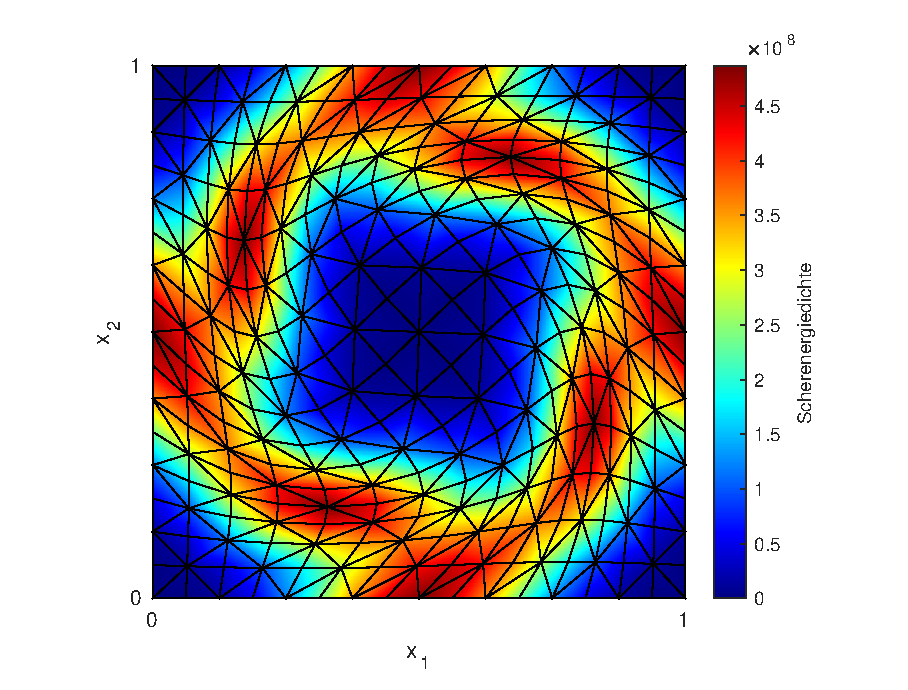
\includegraphics[width=\textwidth]{Plots/SquareBenchmarkDeform5}
\caption{Mögliche Deformation}
\label{pl:SquareBenchmarkDeform}
\end{minipage}
\hfill
\begin{minipage}[t]{0.45\textwidth}
\centering
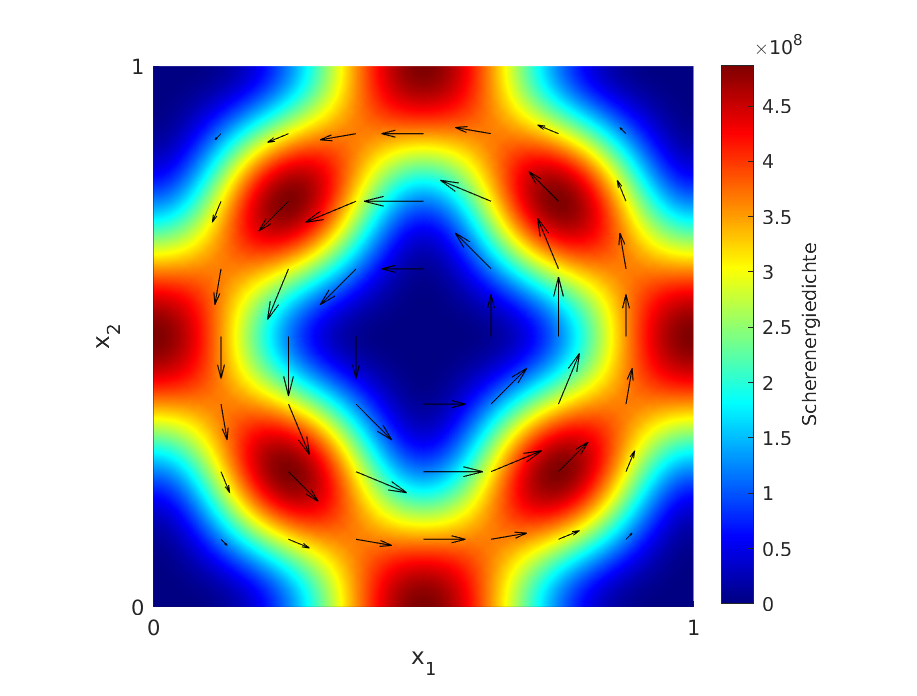
\includegraphics[width=\textwidth]{Plots/SquareBenchmarkSoln3}
\caption{Lösung}
\label{pl:SquareBenmarkSoln}
\end{minipage}
\end{figure}

Das folgende Benchmark stammt aus \cite[Abschnitt 3.1]{Car-2011}.
Wir haben das Gebiet $\Omega=[0,1]^2\subseteq\R^2$ mit reinem Dirichlet-Rand $\Gamma_D=\partial\Omega$, einen festen Parameter $\mu=10^7$ und Funktionen
\begin{align*}
	u(x) = \pi\vect{\cos(\pi x_2)\sin^2(\pi x_1)\sin(\pi x_2) \\
	-\cos( \pi x_1)\sin(\pi  x_1)\sin^2(\pi  x_2)}
\end{align*}
und
\begin{align*}
	f(x) = 2\mu\pi^3\vect{-\cos(\pi x_2)\sin(\pi x_2)(2\cos(2\pi x_1)-1) \\
	\cos(\pi x_1)\sin(\pi x_1)(2\cos(2 \pi x_2)-1)}\,.
\end{align*}
Die Anfangsbedingungen sind in Abbildung \ref{pl:SquareBenchmarkInitial} dargestellt. Die exakte Lösung $u$ und die Scherenergiedichte für $\nu=0.2$ ist in den Plots \ref{pl:SquareBenchmarkDeform} und \ref{pl:SquareBenmarkSoln} zu sehen. Ziel des Experiments ist es, das Lockings nachzuweisen und den residualen Fehlerschätzer zu prüfen. Dazu lassen wir 3 Versuchesreihen mit unterschiedlichen Poissonzahlen $\nu\in\{0.2,0.49,0.499\}$ laufen, in der in jeder Iteration das Gitter uniform verfeinert wird.
\begin{figure}[h]
\centering
\begin{minipage}[t]{0.45\textwidth}
\centering
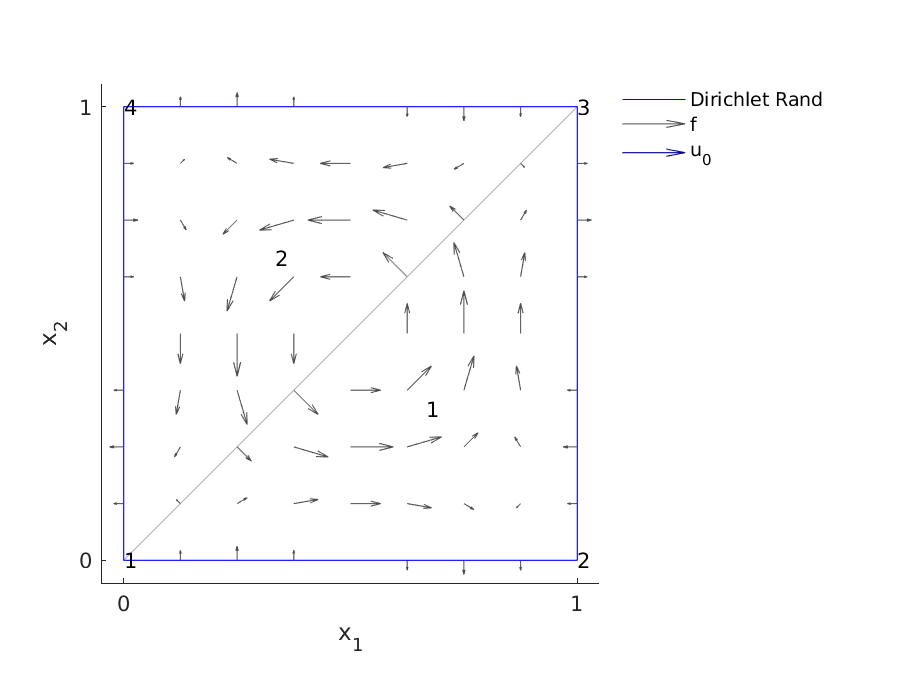
\includegraphics[width=\textwidth]{Plots/SquareBenchmarkInitial3}
\caption{Anfangsbedingungen}
\label{pl:SquareBenchmarkInitial}
\end{minipage}
\hfill
\begin{minipage}[t]{0.45\textwidth}
\centering
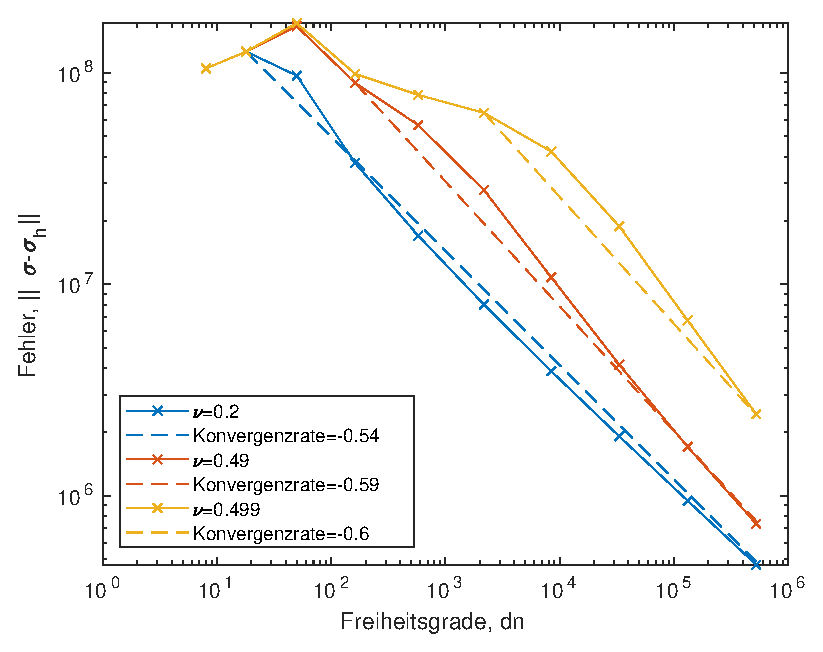
\includegraphics[width=\textwidth]{Plots/SquareBenchmarkNormSigDiff1}
\caption{Fehler}
\label{pl:SquareBenchmarkError}
\end{minipage}
\end{figure}

In Abbildung \ref{pl:SquareBenchmarkError} sieht man eine Näherung des Fehlers $\norm{\sigma(e)}_{0,\Omega}$ in Abhängigkeit der Freiheitsgrade $dn$ geplottet.
Dadurch, dass die Mittelpunktsregel bei der Auswertung der Integrale in $\norm{\sigma(e)}_{0,\Omega}$ verwendet wurde und $\ell$ durch $\ell_H$ approximiert wurde, sind die Daten erst für feinere Gitter aussagekräftig. Allerdings sieht man hier dennoch, dass die Konvergenzrate suboptimal ist für $\nu$ nahe an $1/2$, also, dass Locking auftritt. Man sieht auch, dass die in der Satz \ref{pr:APrioriFehler} vorhergesagten linearen Konvergenzrate annähernd erreicht wird.
Das Locking macht sich auch in der Energie $a(u,u)/2$ in Abbildung \ref{pl:SquareBenchmarkTotalEnergy} und in einer Näherung der Kondition durch \texttt{condest}
in Abbildung \ref{pl:SquareBenchmarkCondition} bemerkbar. Man sieht an der Energie, dass die Lösungen auf dem groben Gitter näher bei der Nulllösung sind, wenn $\nu$ näher am kritischen Wert $1/2$ ist.
Man beachte dabei, dass die ersten beiden berechneten Lösungen in jedem Fall aufgrund der Wahl des Anfangsgitters in Abbildung \ref{pl:SquareBenchmarkInitial} Nulllösungen sind. In der Tat wird beim ersten Verfeinern nur der Mittelpunkt des Quadrats hinzugefügt, wo aufgrund der Symmetrie der Volumenkräfte $f$ um diesen Punkt die Verschiebung Null ist.


\begin{figure}[h]
\centering
\begin{minipage}[b]{0.45\textwidth}
\centering
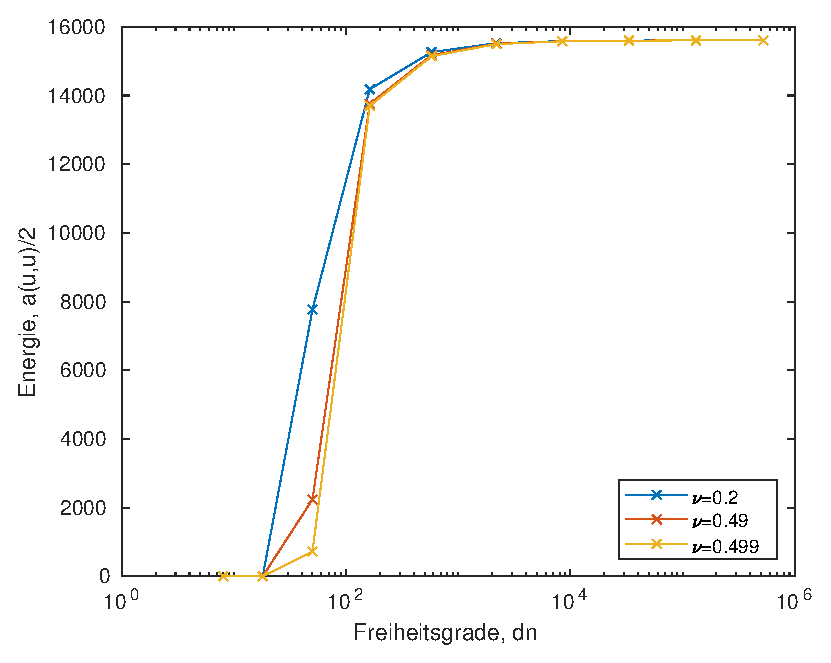
\includegraphics[width=\textwidth]{Plots/SquareBenchmarkTotalEnergy1}
\caption{Energie}
\label{pl:SquareBenchmarkTotalEnergy}
\end{minipage}
\hfill
\begin{minipage}[b]{0.45\textwidth}
\centering
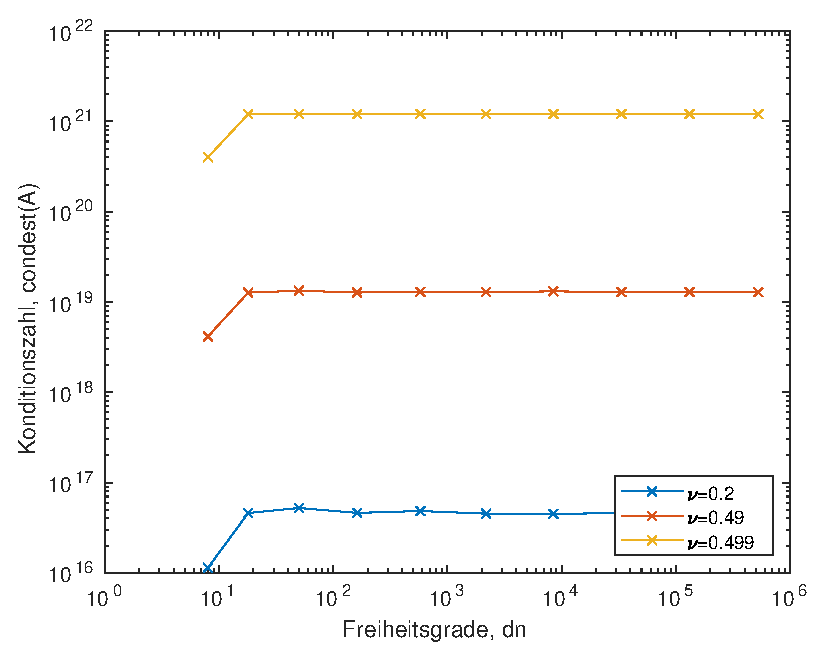
\includegraphics[width=\textwidth]{Plots/SquareBenchmarkCondition1}
\caption{Kondition von $A$}
\label{pl:SquareBenchmarkCondition}
\end{minipage}
\end{figure}
\newpage
In Abbildung \ref{pl:SquareBenchmarkEfficiency} sieht man, dass die in Satz \ref{th:lokaleEffizienz} vorausgesagte lokale Effizienz und die in Satz \ref{th:zuverlaessigkeit} vorhergesagte Zuverlässigkeit erfüllt sind. Der Effizienzindex $\eta_R/\norm{\sigma(e)}_{0,\Omega}$ ist nach oben und nach unten beschränkt und man sieht die Abhängigkeit dieser Schranken vom Materialparameter. Auch hier sind die ersten Messwerte wegen Näherungen der Integrale des Fehlerschätzers und des Fehlers durch die Mittelpunktsregel nicht aussagekräftig.

Ein völlig anderes Verhalten zeigt dagegen der nachfolgend vorgestellte Fehlerschätzer durch Mittelung in Abbildung \ref{pl:SquareBenchmarkInefficiency}. Man beachte das Spektrum an Werten, die der Quotient $\eta_M/\norm{\sigma(e)}_{0,\Omega}$ annimmt.


\begin{figure}[h]
\centering
\begin{minipage}[b]{0.45\textwidth}
\centering
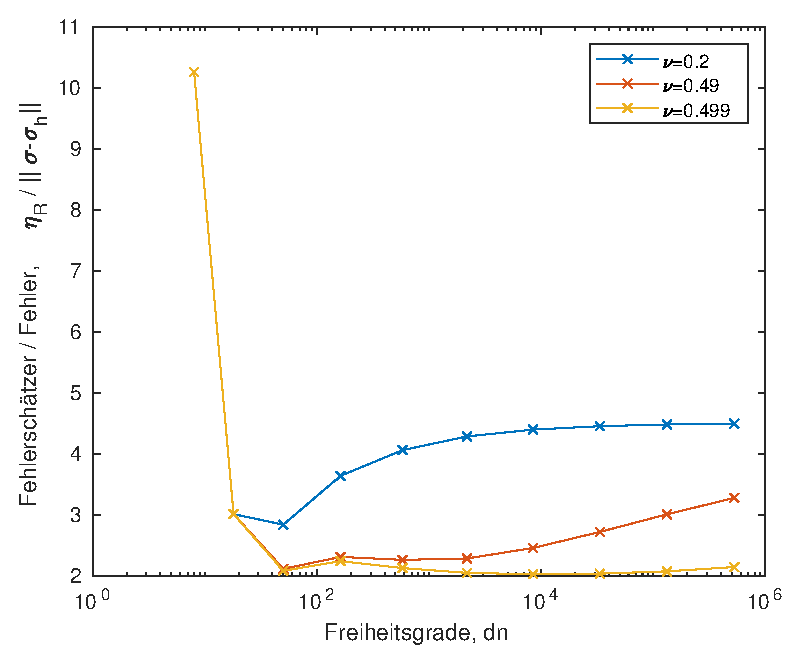
\includegraphics[width=\textwidth]{Plots/SquareBenchmarkEfficiency1}
\caption{Effizienz}
\label{pl:SquareBenchmarkEfficiency}
\end{minipage}
\hfill
\begin{minipage}[b]{0.45\textwidth}
\centering
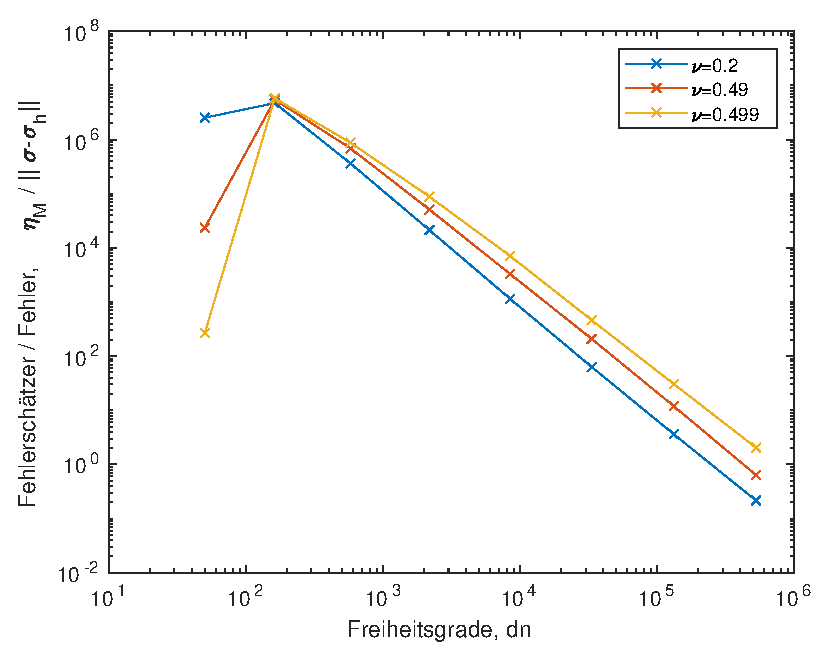
\includegraphics[width=\textwidth]{Plots/SquareBenchmarkInefficiency1}
\caption{Ineffizienz}
\label{pl:SquareBenchmarkInefficiency}
\end{minipage}
\end{figure}

\subsection{Fehlerschätzer durch Mittelung}\label{ch:DefinitionEtaM}

\begin{wrapfigure}{r}{0.45\textwidth}
\centering
%\def\svgwidth{0.2\textwidth}
\input{Drawings/MittelungfehlerschaetzerKonstruktion2.pdf_tex}
\caption{Die Umgebung $\omega_{x^i}$ von $x^i$.}
\label{fig:MittellungsfehlerschaetzerKonstruktion}
\end{wrapfigure}
Wir vergleichen den residualen Fehlerschätzer mit einem Fehlerschätzer durch Mittelung, wie er in \cite[S.253f.]{Alb-2002} beschrieben wird.
Man definiert eine stetige Approximation $\tisigma_h$ an $\sigma_h$, indem man an den Knoten den Wert von $\tisigma_h$ auf das gewichtete Mittel von $\sigma_h\big\vert_T$ der angrenzenden Dreiecke $T\in\cT$ setzt und diesen dann linear auf den Dreiecken interpoliert. Genauer: Für einen Knoten $x^i\in\cN$ definiert man die Umgebung $\omega_{x^i}$ als die Menge aller Dreiecke $T\in\cT$, so dass $x^i$ Knoten von $T$ ist. Man setzt
\begin{align*}
	\tisigma_h(x^i) = \frac{1}{\abs*{\omega_{x^i}}}\sum_{T\in\omega_{x^i}}\abs{T}\cdot\sigma_h\big\vert_{T}
\end{align*}
und Interpoliert $\tisigma_h$ dann linear auf den Dreiecken.
Dies liefert den Fehlerschätzer
\begin{align*}
	\eta_{M,T}\coloneqq\norm{\tisigma_h-\sigma_h}_{0,T}\,.
\end{align*}

\newpage
\subsection{Benchmark: L-förmiges Gebiet}


\begin{figure}[h]
\centering
\begin{minipage}[b]{0.45\textwidth}
\centering
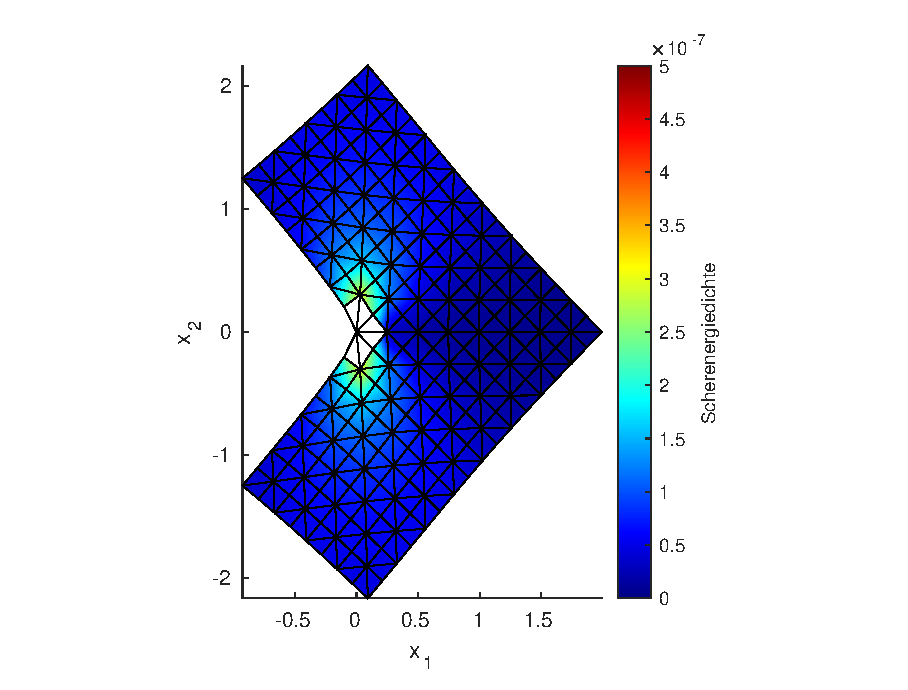
\includegraphics[width=1.3\textwidth]{Plots/LShapeBenchmarkDeform4}
\caption{Mögliche Deformation}
\label{pl:LShapeBenchmarkDeform}
\end{minipage}
\hfill
\begin{minipage}[b]{0.45\textwidth}
\centering
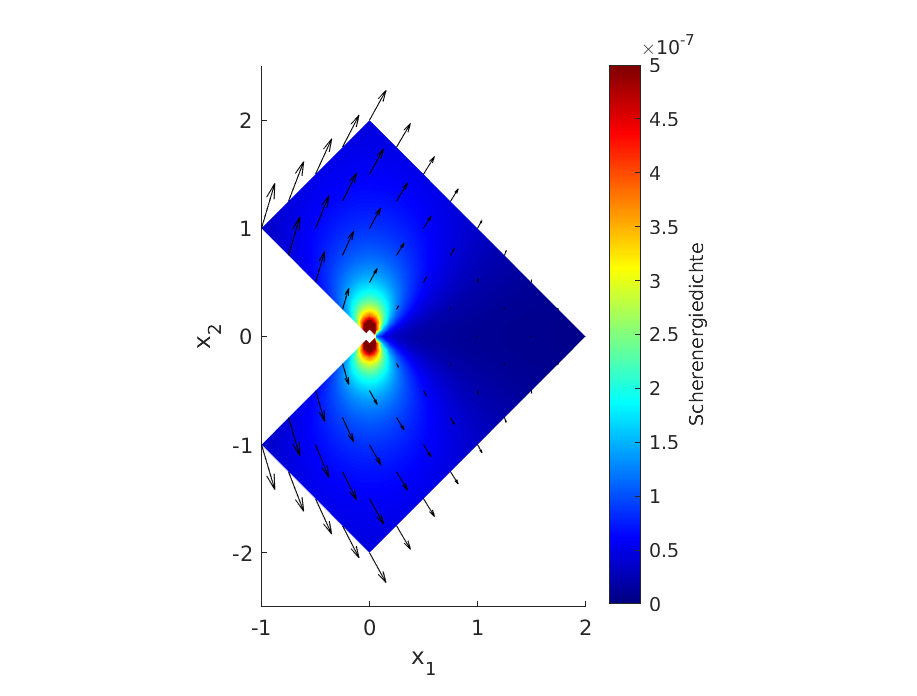
\includegraphics[width=1.3\textwidth]{Plots/LShapeBenchmarkSoln4}
\caption{Lösung}
\label{pl:LShapeBenchmarkSoln}
\end{minipage}
\end{figure}


\begin{figure}[h]
\centering
\begin{minipage}[b]{0.45\textwidth}
\centering
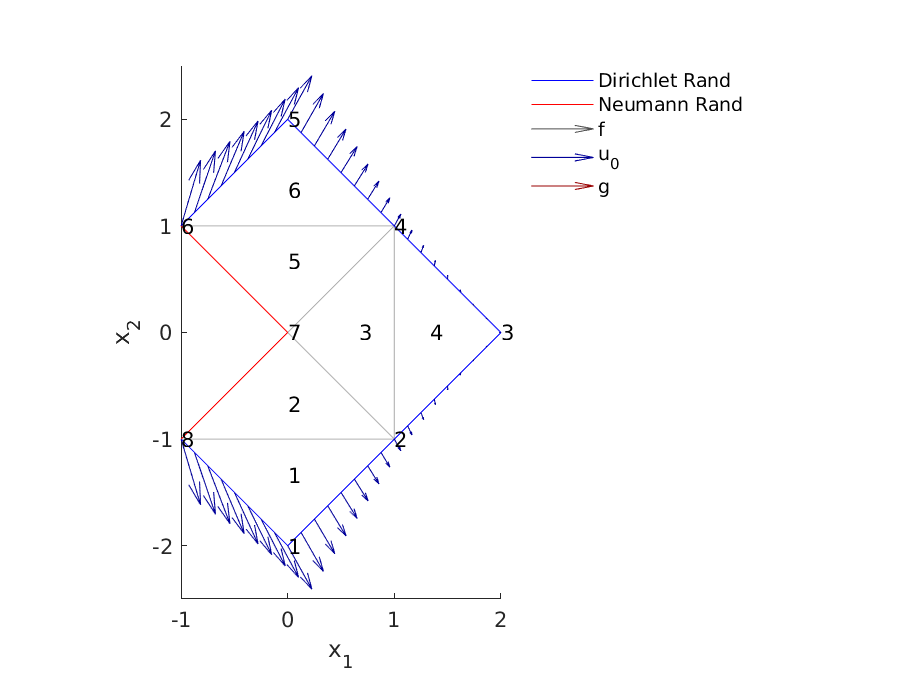
\includegraphics[width=1.3\textwidth]{Plots/LShapeBenchmarkInitial4}
\caption{Anfangsbedingungen}
\label{pl:LShapeBenchmarkInitial}
\end{minipage}
\hfill
\begin{minipage}[b]{0.45\textwidth}
\centering
\scalebox{0.7}{
% Graphic for TeX using PGF
% Title: /mnt/12CCB7B3CCB79009/Filing/Education/University/Bonn/Courses/Bachelorarbeit/Text/Drawings/AdaptiveAlgFlowchart.dia
% Creator: Dia v0.97+git
% CreationDate: Sat Jul  2 20:44:46 2022
% For: theo
% \usepackage{tikz}
% The following commands are not supported in PSTricks at present
% We define them conditionally, so when they are implemented,
% this pgf file will use them.
\ifx\du\undefined
  \newlength{\du}
\fi
\setlength{\du}{15\unitlength}
\begin{tikzpicture}[even odd rule]
\pgftransformxscale{1}
\pgftransformyscale{-1}
\definecolor{dialinecolor}{rgb}{0.000000, 0.000000, 0.000000}
\pgfsetstrokecolor{dialinecolor}
\pgfsetstrokeopacity{1.000000}
\definecolor{diafillcolor}{rgb}{1.000000, 1.000000, 1.000000}
\pgfsetfillcolor{diafillcolor}
\pgfsetfillopacity{1.000000}
\pgfsetlinewidth{0.050000\du}
\pgfsetdash{}{0pt}
\pgfsetmiterjoin
{\pgfsetcornersarced{\pgfpoint{0.000000\du}{0.000000\du}}\definecolor{diafillcolor}{rgb}{1.000000, 1.000000, 1.000000}
\pgfsetfillcolor{diafillcolor}
\pgfsetfillopacity{1.000000}
\fill (-46.022737\du,-5.450000\du)--(-46.022737\du,-2.000000\du)--(-39.112737\du,-2.000000\du)--(-39.112737\du,-5.450000\du)--cycle;
}{\pgfsetcornersarced{\pgfpoint{0.000000\du}{0.000000\du}}\definecolor{dialinecolor}{rgb}{0.000000, 0.000000, 0.000000}
\pgfsetstrokecolor{dialinecolor}
\pgfsetstrokeopacity{1.000000}
\draw (-46.022737\du,-5.450000\du)--(-46.022737\du,-2.000000\du)--(-39.112737\du,-2.000000\du)--(-39.112737\du,-5.450000\du)--cycle;
}% setfont left to latex
\definecolor{dialinecolor}{rgb}{0.000000, 0.000000, 0.000000}
\pgfsetstrokecolor{dialinecolor}
\pgfsetstrokeopacity{1.000000}
\definecolor{diafillcolor}{rgb}{0.000000, 0.000000, 0.000000}
\pgfsetfillcolor{diafillcolor}
\pgfsetfillopacity{1.000000}
\node[anchor=base,inner sep=0pt, outer sep=0pt,color=dialinecolor] at (-42.567737\du,-4.330947\du){markiere Dreiecke};
% setfont left to latex
\definecolor{dialinecolor}{rgb}{0.000000, 0.000000, 0.000000}
\pgfsetstrokecolor{dialinecolor}
\pgfsetstrokeopacity{1.000000}
\definecolor{diafillcolor}{rgb}{0.000000, 0.000000, 0.000000}
\pgfsetfillcolor{diafillcolor}
\pgfsetfillopacity{1.000000}
\node[anchor=base,inner sep=0pt, outer sep=0pt,color=dialinecolor] at (-42.567737\du,-3.530947\du){zur Verfeinerung};
% setfont left to latex
\definecolor{dialinecolor}{rgb}{0.000000, 0.000000, 0.000000}
\pgfsetstrokecolor{dialinecolor}
\pgfsetstrokeopacity{1.000000}
\definecolor{diafillcolor}{rgb}{0.000000, 0.000000, 0.000000}
\pgfsetfillcolor{diafillcolor}
\pgfsetfillopacity{1.000000}
\node[anchor=base,inner sep=0pt, outer sep=0pt,color=dialinecolor] at (-42.567737\du,-2.730947\du){mit \texttt{MARK.m}};
\pgfsetlinewidth{0.050000\du}
\pgfsetdash{}{0pt}
\pgfsetmiterjoin
{\pgfsetcornersarced{\pgfpoint{0.000000\du}{0.000000\du}}\definecolor{diafillcolor}{rgb}{1.000000, 1.000000, 1.000000}
\pgfsetfillcolor{diafillcolor}
\pgfsetfillopacity{1.000000}
\fill (-45.227263\du,-0.986369\du)--(-45.227263\du,1.663631\du)--(-39.899763\du,1.663631\du)--(-39.899763\du,-0.986369\du)--cycle;
}{\pgfsetcornersarced{\pgfpoint{0.000000\du}{0.000000\du}}\definecolor{dialinecolor}{rgb}{0.000000, 0.000000, 0.000000}
\pgfsetstrokecolor{dialinecolor}
\pgfsetstrokeopacity{1.000000}
\draw (-45.227263\du,-0.986369\du)--(-45.227263\du,1.663631\du)--(-39.899763\du,1.663631\du)--(-39.899763\du,-0.986369\du)--cycle;
}% setfont left to latex
\definecolor{dialinecolor}{rgb}{0.000000, 0.000000, 0.000000}
\pgfsetstrokecolor{dialinecolor}
\pgfsetstrokeopacity{1.000000}
\definecolor{diafillcolor}{rgb}{0.000000, 0.000000, 0.000000}
\pgfsetfillcolor{diafillcolor}
\pgfsetfillopacity{1.000000}
\node[anchor=base,inner sep=0pt, outer sep=0pt,color=dialinecolor] at (-42.563513\du,0.132684\du){Verfeinerung};
% setfont left to latex
\definecolor{dialinecolor}{rgb}{0.000000, 0.000000, 0.000000}
\pgfsetstrokecolor{dialinecolor}
\pgfsetstrokeopacity{1.000000}
\definecolor{diafillcolor}{rgb}{0.000000, 0.000000, 0.000000}
\pgfsetfillcolor{diafillcolor}
\pgfsetfillopacity{1.000000}
\node[anchor=base,inner sep=0pt, outer sep=0pt,color=dialinecolor] at (-42.563513\du,0.932684\du){mit \texttt{BISECT.m}};
\pgfsetlinewidth{0.050000\du}
\pgfsetdash{}{0pt}
\pgfsetmiterjoin
{\pgfsetcornersarced{\pgfpoint{0.000000\du}{0.000000\du}}\definecolor{diafillcolor}{rgb}{1.000000, 1.000000, 1.000000}
\pgfsetfillcolor{diafillcolor}
\pgfsetfillopacity{1.000000}
\fill (-45.904581\du,-13.595976\du)--(-45.904581\du,-10.945976\du)--(-39.252081\du,-10.945976\du)--(-39.252081\du,-13.595976\du)--cycle;
}{\pgfsetcornersarced{\pgfpoint{0.000000\du}{0.000000\du}}\definecolor{dialinecolor}{rgb}{0.000000, 0.000000, 0.000000}
\pgfsetstrokecolor{dialinecolor}
\pgfsetstrokeopacity{1.000000}
\draw (-45.904581\du,-13.595976\du)--(-45.904581\du,-10.945976\du)--(-39.252081\du,-10.945976\du)--(-39.252081\du,-13.595976\du)--cycle;
}% setfont left to latex
\definecolor{dialinecolor}{rgb}{0.000000, 0.000000, 0.000000}
\pgfsetstrokecolor{dialinecolor}
\pgfsetstrokeopacity{1.000000}
\definecolor{diafillcolor}{rgb}{0.000000, 0.000000, 0.000000}
\pgfsetfillcolor{diafillcolor}
\pgfsetfillopacity{1.000000}
\node[anchor=base,inner sep=0pt, outer sep=0pt,color=dialinecolor] at (-42.578331\du,-12.476924\du){Schätze Fehler};
% setfont left to latex
\definecolor{dialinecolor}{rgb}{0.000000, 0.000000, 0.000000}
\pgfsetstrokecolor{dialinecolor}
\pgfsetstrokeopacity{1.000000}
\definecolor{diafillcolor}{rgb}{0.000000, 0.000000, 0.000000}
\pgfsetfillcolor{diafillcolor}
\pgfsetfillopacity{1.000000}
\node[anchor=base,inner sep=0pt, outer sep=0pt,color=dialinecolor] at (-42.578331\du,-11.676924\du){mit $\eta_{R,T}$ oder $\eta_{M,T}$};
% setfont left to latex
\definecolor{dialinecolor}{rgb}{0.000000, 0.000000, 0.000000}
\pgfsetstrokecolor{dialinecolor}
\pgfsetstrokeopacity{1.000000}
\definecolor{diafillcolor}{rgb}{0.000000, 0.000000, 0.000000}
\pgfsetfillcolor{diafillcolor}
\pgfsetfillopacity{1.000000}
\node[anchor=base west,inner sep=0pt,outer sep=0pt,color=dialinecolor] at (-42.567737\du,-3.725000\du){};
\pgfsetlinewidth{0.050000\du}
\pgfsetdash{}{0pt}
\pgfsetmiterjoin
{\pgfsetcornersarced{\pgfpoint{0.000000\du}{0.000000\du}}\definecolor{diafillcolor}{rgb}{1.000000, 1.000000, 1.000000}
\pgfsetfillcolor{diafillcolor}
\pgfsetfillopacity{1.000000}
\fill (-46.618324\du,-17.214300\du)--(-46.618324\du,-14.564300\du)--(-38.495824\du,-14.564300\du)--(-38.495824\du,-17.214300\du)--cycle;
}{\pgfsetcornersarced{\pgfpoint{0.000000\du}{0.000000\du}}\definecolor{dialinecolor}{rgb}{0.000000, 0.000000, 0.000000}
\pgfsetstrokecolor{dialinecolor}
\pgfsetstrokeopacity{1.000000}
\draw (-46.618324\du,-17.214300\du)--(-46.618324\du,-14.564300\du)--(-38.495824\du,-14.564300\du)--(-38.495824\du,-17.214300\du)--cycle;
}% setfont left to latex
\definecolor{dialinecolor}{rgb}{0.000000, 0.000000, 0.000000}
\pgfsetstrokecolor{dialinecolor}
\pgfsetstrokeopacity{1.000000}
\definecolor{diafillcolor}{rgb}{0.000000, 0.000000, 0.000000}
\pgfsetfillcolor{diafillcolor}
\pgfsetfillopacity{1.000000}
\node[anchor=base,inner sep=0pt, outer sep=0pt,color=dialinecolor] at (-42.557074\du,-16.095247\du){Löse das diskrete};
% setfont left to latex
\definecolor{dialinecolor}{rgb}{0.000000, 0.000000, 0.000000}
\pgfsetstrokecolor{dialinecolor}
\pgfsetstrokeopacity{1.000000}
\definecolor{diafillcolor}{rgb}{0.000000, 0.000000, 0.000000}
\pgfsetfillcolor{diafillcolor}
\pgfsetfillopacity{1.000000}
\node[anchor=base,inner sep=0pt, outer sep=0pt,color=dialinecolor] at (-42.557074\du,-15.295247\du){Problem mit \texttt{ECFEM.m}};
\pgfsetlinewidth{0.050000\du}
\pgfsetdash{}{0pt}
\pgfsetmiterjoin
{\pgfsetcornersarced{\pgfpoint{0.000000\du}{0.000000\du}}\definecolor{diafillcolor}{rgb}{1.000000, 1.000000, 1.000000}
\pgfsetfillcolor{diafillcolor}
\pgfsetfillopacity{1.000000}
\fill (-43.851330\du,-20.461577\du)--(-43.851330\du,-18.611577\du)--(-41.241330\du,-18.611577\du)--(-41.241330\du,-20.461577\du)--cycle;
}{\pgfsetcornersarced{\pgfpoint{0.000000\du}{0.000000\du}}\definecolor{dialinecolor}{rgb}{0.000000, 0.000000, 0.000000}
\pgfsetstrokecolor{dialinecolor}
\pgfsetstrokeopacity{1.000000}
\draw (-43.851330\du,-20.461577\du)--(-43.851330\du,-18.611577\du)--(-41.241330\du,-18.611577\du)--(-41.241330\du,-20.461577\du)--cycle;
}% setfont left to latex
\definecolor{dialinecolor}{rgb}{0.000000, 0.000000, 0.000000}
\pgfsetstrokecolor{dialinecolor}
\pgfsetstrokeopacity{1.000000}
\definecolor{diafillcolor}{rgb}{0.000000, 0.000000, 0.000000}
\pgfsetfillcolor{diafillcolor}
\pgfsetfillopacity{1.000000}
\node[anchor=base,inner sep=0pt, outer sep=0pt,color=dialinecolor] at (-42.546330\du,-19.342524\du){Start};
\pgfsetlinewidth{0.050000\du}
\pgfsetdash{}{0pt}
\pgfsetbuttcap
{
\definecolor{diafillcolor}{rgb}{0.000000, 0.000000, 0.000000}
\pgfsetfillcolor{diafillcolor}
\pgfsetfillopacity{1.000000}
% was here!!!
\pgfsetarrowsend{latex}
\definecolor{dialinecolor}{rgb}{0.000000, 0.000000, 0.000000}
\pgfsetstrokecolor{dialinecolor}
\pgfsetstrokeopacity{1.000000}
\draw (-42.557074\du,-14.564300\du)--(-42.578331\du,-13.595976\du);
}
\pgfsetlinewidth{0.050000\du}
\pgfsetdash{}{0pt}
\pgfsetbuttcap
{
\definecolor{diafillcolor}{rgb}{0.000000, 0.000000, 0.000000}
\pgfsetfillcolor{diafillcolor}
\pgfsetfillopacity{1.000000}
% was here!!!
\pgfsetarrowsend{latex}
\definecolor{dialinecolor}{rgb}{0.000000, 0.000000, 0.000000}
\pgfsetstrokecolor{dialinecolor}
\pgfsetstrokeopacity{1.000000}
\draw (-42.567737\du,-2.000000\du)--(-42.563513\du,-0.986369\du);
}
\pgfsetlinewidth{0.050000\du}
\pgfsetdash{}{0pt}
\pgfsetmiterjoin
{\pgfsetcornersarced{\pgfpoint{0.000000\du}{0.000000\du}}\definecolor{diafillcolor}{rgb}{1.000000, 1.000000, 1.000000}
\pgfsetfillcolor{diafillcolor}
\pgfsetfillopacity{1.000000}
\fill (-46.000000\du,-9.950000\du)--(-46.000000\du,-6.500000\du)--(-39.155000\du,-6.500000\du)--(-39.155000\du,-9.950000\du)--cycle;
}{\pgfsetcornersarced{\pgfpoint{0.000000\du}{0.000000\du}}\definecolor{dialinecolor}{rgb}{0.000000, 0.000000, 0.000000}
\pgfsetstrokecolor{dialinecolor}
\pgfsetstrokeopacity{1.000000}
\draw (-46.000000\du,-9.950000\du)--(-46.000000\du,-6.500000\du)--(-39.155000\du,-6.500000\du)--(-39.155000\du,-9.950000\du)--cycle;
}% setfont left to latex
\definecolor{dialinecolor}{rgb}{0.000000, 0.000000, 0.000000}
\pgfsetstrokecolor{dialinecolor}
\pgfsetstrokeopacity{1.000000}
\definecolor{diafillcolor}{rgb}{0.000000, 0.000000, 0.000000}
\pgfsetfillcolor{diafillcolor}
\pgfsetfillopacity{1.000000}
\node[anchor=base,inner sep=0pt, outer sep=0pt,color=dialinecolor] at (-42.577500\du,-8.830947\du){Entscheide, ob};
% setfont left to latex
\definecolor{dialinecolor}{rgb}{0.000000, 0.000000, 0.000000}
\pgfsetstrokecolor{dialinecolor}
\pgfsetstrokeopacity{1.000000}
\definecolor{diafillcolor}{rgb}{0.000000, 0.000000, 0.000000}
\pgfsetfillcolor{diafillcolor}
\pgfsetfillopacity{1.000000}
\node[anchor=base,inner sep=0pt, outer sep=0pt,color=dialinecolor] at (-42.577500\du,-8.030947\du){Abbruchkriterium};
% setfont left to latex
\definecolor{dialinecolor}{rgb}{0.000000, 0.000000, 0.000000}
\pgfsetstrokecolor{dialinecolor}
\pgfsetstrokeopacity{1.000000}
\definecolor{diafillcolor}{rgb}{0.000000, 0.000000, 0.000000}
\pgfsetfillcolor{diafillcolor}
\pgfsetfillopacity{1.000000}
\node[anchor=base,inner sep=0pt, outer sep=0pt,color=dialinecolor] at (-42.577500\du,-7.230947\du){erfüllt ist};
\pgfsetlinewidth{0.050000\du}
\pgfsetdash{}{0pt}
\pgfsetmiterjoin
{\pgfsetcornersarced{\pgfpoint{0.000000\du}{0.000000\du}}\definecolor{diafillcolor}{rgb}{1.000000, 1.000000, 1.000000}
\pgfsetfillcolor{diafillcolor}
\pgfsetfillopacity{1.000000}
\fill (-38.067042\du,-9.182122\du)--(-38.067042\du,-7.332122\du)--(-35.564542\du,-7.332122\du)--(-35.564542\du,-9.182122\du)--cycle;
}{\pgfsetcornersarced{\pgfpoint{0.000000\du}{0.000000\du}}\definecolor{dialinecolor}{rgb}{0.000000, 0.000000, 0.000000}
\pgfsetstrokecolor{dialinecolor}
\pgfsetstrokeopacity{1.000000}
\draw (-38.067042\du,-9.182122\du)--(-38.067042\du,-7.332122\du)--(-35.564542\du,-7.332122\du)--(-35.564542\du,-9.182122\du)--cycle;
}% setfont left to latex
\definecolor{dialinecolor}{rgb}{0.000000, 0.000000, 0.000000}
\pgfsetstrokecolor{dialinecolor}
\pgfsetstrokeopacity{1.000000}
\definecolor{diafillcolor}{rgb}{0.000000, 0.000000, 0.000000}
\pgfsetfillcolor{diafillcolor}
\pgfsetfillopacity{1.000000}
\node[anchor=base,inner sep=0pt, outer sep=0pt,color=dialinecolor] at (-36.815792\du,-8.063069\du){Stop};
\pgfsetlinewidth{0.050000\du}
\pgfsetdash{}{0pt}
\pgfsetbuttcap
{
\definecolor{diafillcolor}{rgb}{0.000000, 0.000000, 0.000000}
\pgfsetfillcolor{diafillcolor}
\pgfsetfillopacity{1.000000}
% was here!!!
\pgfsetarrowsend{latex}
\definecolor{dialinecolor}{rgb}{0.000000, 0.000000, 0.000000}
\pgfsetstrokecolor{dialinecolor}
\pgfsetstrokeopacity{1.000000}
\draw (-42.577500\du,-6.500000\du)--(-42.567737\du,-5.450000\du);
}
\pgfsetlinewidth{0.050000\du}
\pgfsetdash{}{0pt}
\pgfsetbuttcap
{
\definecolor{diafillcolor}{rgb}{0.000000, 0.000000, 0.000000}
\pgfsetfillcolor{diafillcolor}
\pgfsetfillopacity{1.000000}
% was here!!!
\pgfsetarrowsend{latex}
\definecolor{dialinecolor}{rgb}{0.000000, 0.000000, 0.000000}
\pgfsetstrokecolor{dialinecolor}
\pgfsetstrokeopacity{1.000000}
\draw (-42.578331\du,-10.945976\du)--(-42.577500\du,-9.950000\du);
}
\pgfsetlinewidth{0.050000\du}
\pgfsetdash{}{0pt}
\pgfsetbuttcap
{
\definecolor{diafillcolor}{rgb}{0.000000, 0.000000, 0.000000}
\pgfsetfillcolor{diafillcolor}
\pgfsetfillopacity{1.000000}
% was here!!!
\pgfsetarrowsend{latex}
\definecolor{dialinecolor}{rgb}{0.000000, 0.000000, 0.000000}
\pgfsetstrokecolor{dialinecolor}
\pgfsetstrokeopacity{1.000000}
\draw (-39.130237\du,-8.249550\du)--(-38.067042\du,-8.257122\du);
}
\pgfsetlinewidth{0.050000\du}
\pgfsetdash{}{0pt}
\pgfsetbuttcap
{
\definecolor{diafillcolor}{rgb}{0.000000, 0.000000, 0.000000}
\pgfsetfillcolor{diafillcolor}
\pgfsetfillopacity{1.000000}
% was here!!!
\pgfsetarrowsend{latex}
\definecolor{dialinecolor}{rgb}{0.000000, 0.000000, 0.000000}
\pgfsetstrokecolor{dialinecolor}
\pgfsetstrokeopacity{1.000000}
\draw (-42.550721\du,-18.587482\du)--(-42.557074\du,-17.214300\du);
}
\pgfsetlinewidth{0.050000\du}
\pgfsetdash{}{0pt}
\pgfsetbuttcap
{
\definecolor{diafillcolor}{rgb}{0.000000, 0.000000, 0.000000}
\pgfsetfillcolor{diafillcolor}
\pgfsetfillopacity{1.000000}
% was here!!!
\definecolor{dialinecolor}{rgb}{0.000000, 0.000000, 0.000000}
\pgfsetstrokecolor{dialinecolor}
\pgfsetstrokeopacity{1.000000}
\draw (-42.576012\du,1.694881\du)--(-42.572138\du,2.710680\du);
}
\pgfsetlinewidth{0.050000\du}
\pgfsetdash{}{0pt}
\pgfsetbuttcap
{
\definecolor{diafillcolor}{rgb}{0.000000, 0.000000, 0.000000}
\pgfsetfillcolor{diafillcolor}
\pgfsetfillopacity{1.000000}
% was here!!!
\definecolor{dialinecolor}{rgb}{0.000000, 0.000000, 0.000000}
\pgfsetstrokecolor{dialinecolor}
\pgfsetstrokeopacity{1.000000}
\draw (-42.587413\du,2.686220\du)--(-48.200000\du,2.700000\du);
}
\pgfsetlinewidth{0.050000\du}
\pgfsetdash{}{0pt}
\pgfsetbuttcap
{
\definecolor{diafillcolor}{rgb}{0.000000, 0.000000, 0.000000}
\pgfsetfillcolor{diafillcolor}
\pgfsetfillopacity{1.000000}
% was here!!!
\definecolor{dialinecolor}{rgb}{0.000000, 0.000000, 0.000000}
\pgfsetstrokecolor{dialinecolor}
\pgfsetstrokeopacity{1.000000}
\draw (-48.200000\du,2.700000\du)--(-48.200000\du,-17.900000\du);
}
\pgfsetlinewidth{0.050000\du}
\pgfsetdash{}{0pt}
\pgfsetbuttcap
{
\definecolor{diafillcolor}{rgb}{0.000000, 0.000000, 0.000000}
\pgfsetfillcolor{diafillcolor}
\pgfsetfillopacity{1.000000}
% was here!!!
\pgfsetarrowsend{latex}
\definecolor{dialinecolor}{rgb}{0.000000, 0.000000, 0.000000}
\pgfsetstrokecolor{dialinecolor}
\pgfsetstrokeopacity{1.000000}
\draw (-48.200000\du,-17.900000\du)--(-42.553897\du,-17.900891\du);
}
\end{tikzpicture}

}
\caption{Adaptiven Gitterverfeinerung}
\label{fc:AdaptiveAlgFlowchart}
\end{minipage}
\end{figure}

Das folgende Benchmark stammt aus \cite[Abschnitt 3.4]{Car-2011} und \cite[S.255f.]{Alb-2002}.
Wir verwenden ein L-förmiges Gebiet mit Dirichlet- und Neumann-Rand wie in Abbildung \ref{pl:LShapeBenchmarkInitial} dargestellt.
Wir setzen weiter $\mu=10^7$ und $\nu=0.3$. Die Verschiebung $u$ ist
in Polarkoordinaten gegeben durch
\begin{align*}
	u_r(r,\varphi) &= \frac{r^\alpha}{2\mu}\big(-(\alpha+1)\cos\left((\alpha+1)\varphi\right) \\
	&\qquad\qquad+(C_2-\alpha-1)C_1\cos\left((\alpha-1)\varphi\right)\big) \\
	u_\varphi(r,\varphi) &= \frac{r^\alpha}{2\mu}\big((\alpha+1)\sin\left((\alpha+1)\varphi\right) \\
	&\qquad\qquad+(C_2+\alpha-1)C_1\sin\left((\alpha-1)\varphi\right)\big)
\end{align*}
mit Konstanten
\begin{align*}
	C_1\coloneqq -\frac{\cos((\alpha+1)\omega)}{\cos((\alpha-1)\omega)},
	\quad C_2\coloneqq2\frac{\lambda+2\mu}{\lambda+\mu},
	\quad\alpha\approx 0.544483736782,
	\quad\omega\coloneqq\frac{3\pi}{4}
\end{align*}
nach \cite[Abschnitt 3.4]{Car-2011}.
Weiter setzen wir $f = 0$ und $g=0$.
Die exakte Lösung $u$ sieht man in Abbildungen \ref{pl:LShapeBenchmarkDeform} und \ref{pl:LShapeBenchmarkSoln}. 
In diesem Experiment wird die Art der Verfeinerung zwischen uniform und adaptiv mit Fehlerschätzern $\eta_R$ und $\eta_M$ variiert.
In Abbildung \ref{fc:AdaptiveAlgFlowchart} ist die Routine für die adaptive Gitterverfeinerung dargestellt.
Das markieren in der Funktion \texttt{MARK.m} erfolgt nach der Methode von Dörfler in \cite{Doe-1996}. Hierbei werden für einen Parameter $\zeta\in(0,1)$ solange die Dreiecke $T\in\cT$ mit den größten Fehlerschätzungen $\eta_{T,R}$ markiert, bis
\begin{align*}
	\sum_{T\text{ markiert}}\eta_{R,T}^2\geq\zeta\eta_R^2
\end{align*}
erfüllt ist. In diesem Experiment wurde $\zeta=0.7$ gesetzt. Für die Gitterverfeinerung wird in \texttt{BISECT.m} ein Bisektionsalgorithmus verwendet, der auf dem Zerteilen der längsten Kante basiert.

Da dieses Problem eine Singularität im Ursprung hat und wir $u\in H^2(\Omega;\R^d)$ für die a priori Abschätzung in Satz \ref{pr:APrioriFehler} benötigen, ist lineare Konvergenz des Fehlers in $h$ nicht mehr garantiert. In der Tat konvergiert die uniforme Verfeinerung nicht mehr linear, wie in Abbildung \ref{pl:AdaptivityBenchmarkNormSigDiff} zu erkennen ist. Die adaptive Verfeinerung mit dem residualen Fehlerschätzer liefert dagegen wieder die optimale Konvergenzrate für das Verfahren. Bei der adaptiven Verfeinerung mit dem Fehlerschätzer $\eta_M$ wird die Steifheitsmatrix bei $d\cdot n\approx3000$ Freiheitsgraden singulär, was sich interessanterweise nicht in der Kondition in Abbildung \ref{pl:AdaptivityBenchmarkCondition} bemerkbar macht.
Der Grund für dieses Verhalten liegt darin, dass der Mittelungsfehlerschätzer erfolgreich eine Singularität im Ursprung erkennt, diese aber zu stark gewichtet, so dass fast ausschließlich die Dreiecke am Ursprung verfeinert werden. Dieses Verhalten sieht man in den Abbildungen \ref{pl:LShapeLocalEtaR}-\ref{pl:LShapeLocalNormSigDiff1506}. 


\begin{figure}[h]
\centering
\begin{minipage}[b]{0.45\textwidth}
\centering
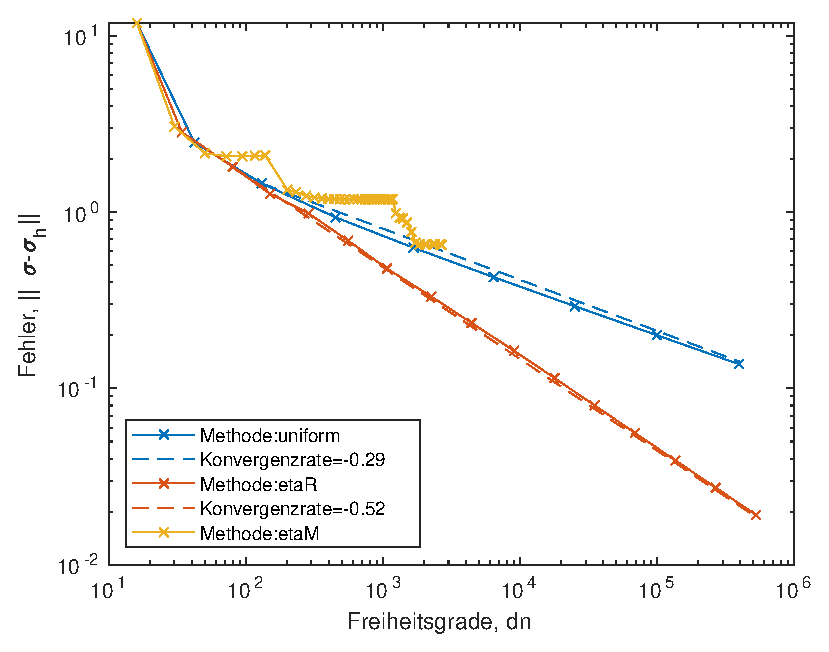
\includegraphics[width=\textwidth]{Plots/AdaptivityBenchmarkNormSigDiff1}
\caption{Fehler}
\label{pl:AdaptivityBenchmarkNormSigDiff}
\end{minipage}
\hfill
\begin{minipage}[b]{0.45\textwidth}
\centering
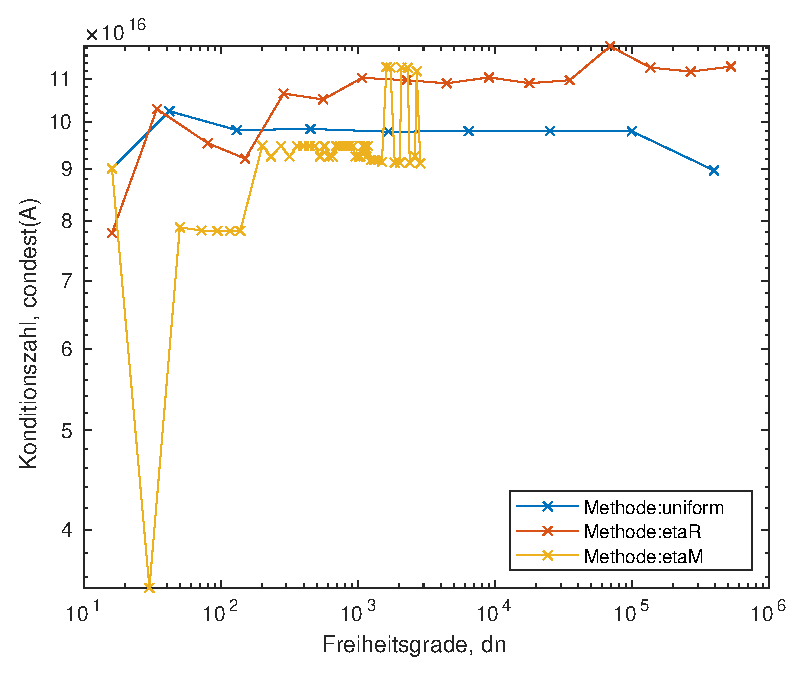
\includegraphics[width=1\textwidth]{Plots/AdaptivityBenchmarkCondition1}
\caption{Kondition}
\label{pl:AdaptivityBenchmarkCondition}
\end{minipage}
\end{figure}
In Abbildung \ref{pl:AdaptivityBenchmarkInefficiency} sieht man, dass der Fehlerschätzer durch Mittelung auch bei diesem Problem nicht zuverlässig ist.
Der residuale Fehlerschätzer $\eta_R$ weist dagegen wie im ersten Benchmark in Abbildung \ref{pl:AdaptivityBenchmarkEfficiency} Effizienz und Zuverlässigkeit auf.


\begin{figure}[h]
\centering
\begin{minipage}[b]{0.45\textwidth}
\centering
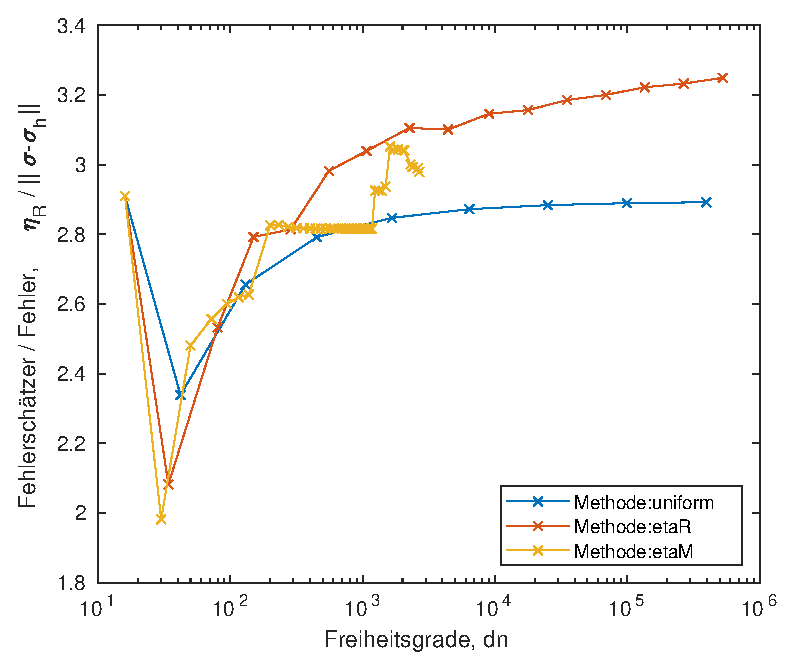
\includegraphics[width=1\textwidth]{Plots/AdaptivityBenchmarkEfficiency1}
\caption{Effizienz}
\label{pl:AdaptivityBenchmarkEfficiency}
\end{minipage}
\hfill
\begin{minipage}[b]{0.45\textwidth}
\centering
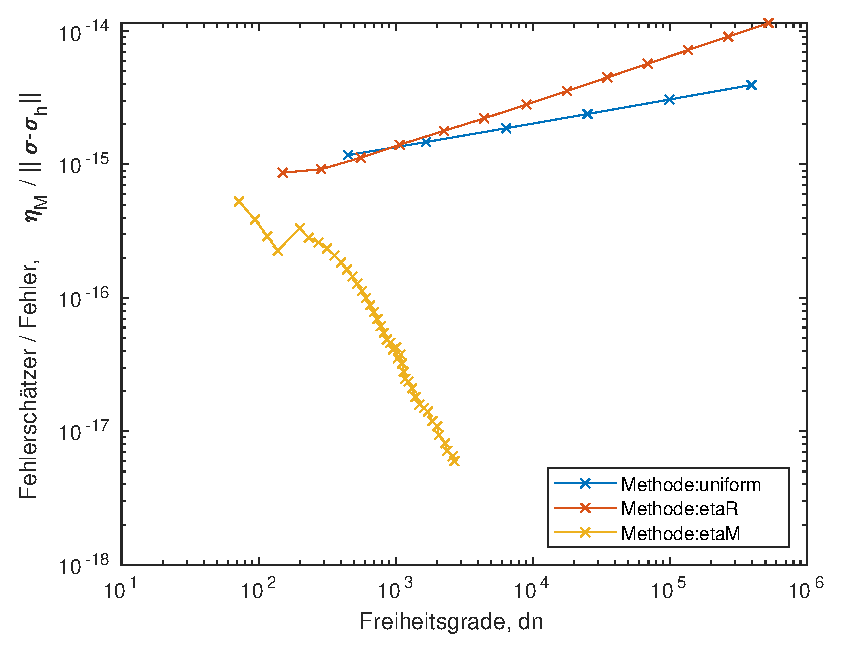
\includegraphics[width=\textwidth]{Plots/AdaptivityBenchmarkInefficiency1}
\caption{Ineffizienz}
\label{pl:AdaptivityBenchmarkInefficiency}
\end{minipage}
\end{figure}

\begin{figure}[h]
\centering
\begin{subfigure}[b]{0.45\textwidth}
\centering
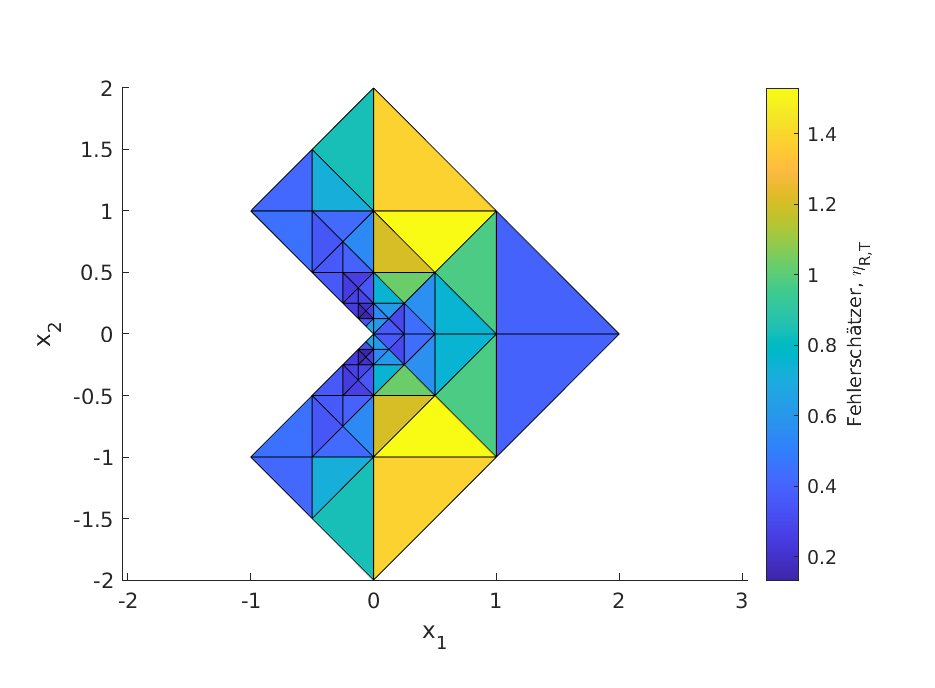
\includegraphics[width=\textwidth]{Plots/LShapeBenchmarkLocaletaR94}
\caption{lokaler Fehlerschätzer $\eta_{R,T}$}
\label{pl:LShapeLocalEtaR}
\end{subfigure}
\hfill
\begin{subfigure}[b]{0.45\textwidth}
\centering
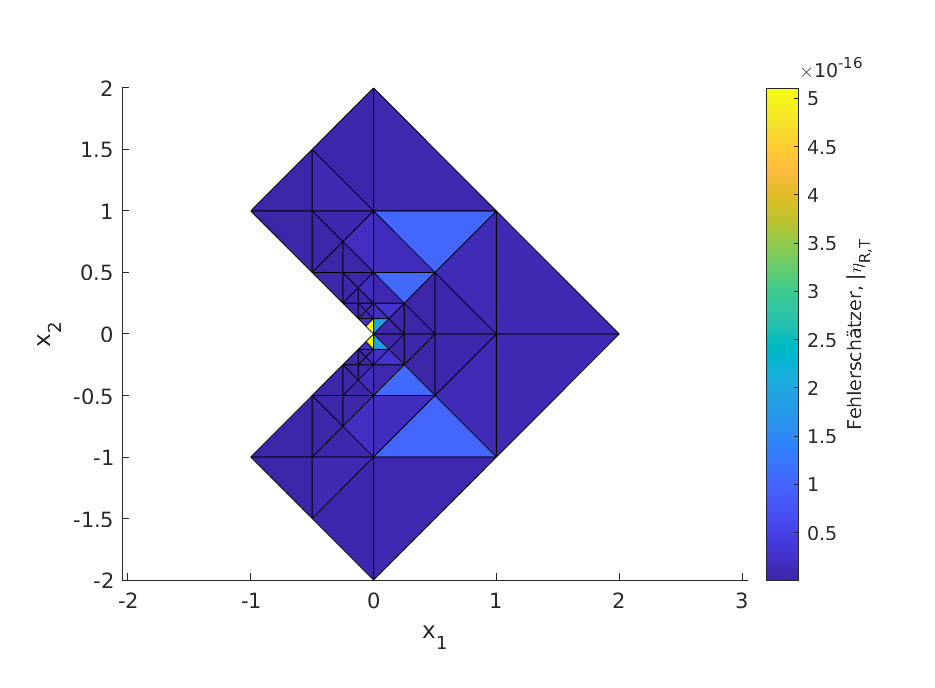
\includegraphics[width=\textwidth]{Plots/LShapeBenchmarkLocaletaM94}
\caption{lokaler Fehlerschätzer $\eta_{M,T}$}
\label{pl:LShapeLocalEtaM}
\end{subfigure}

\begin{subfigure}[b]{0.45\textwidth}
\centering
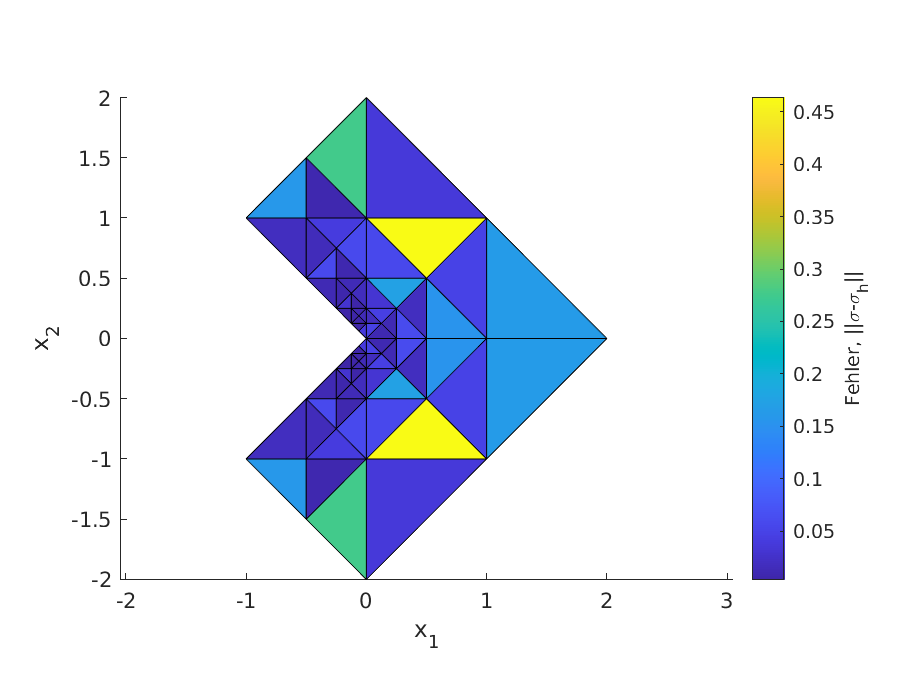
\includegraphics[width=\textwidth]{Plots/LShapeBenchmarkLocalNormSigDiff94}
\caption{lokaler Fehler $\norm{\sigma-\sigma_h}$}
\end{subfigure}
\hfill
\begin{subfigure}[b]{0.45\textwidth}
\centering
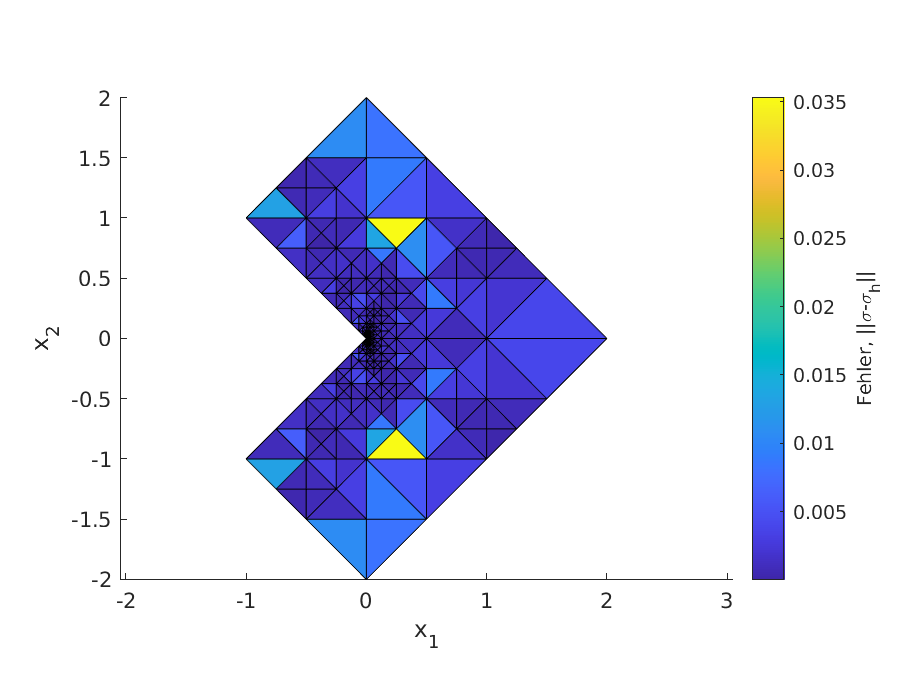
\includegraphics[width=\textwidth]{Plots/LShapeBenchmarkLocalNormSigDiff1610}
\caption{lokaler Fehler $\norm{\sigma-\sigma_h}$}
\label{pl:LShapeLocalNormSigDiff1506}
\end{subfigure}
\caption{Adaptive Gitterverfeinerung mit dem Mittelungsfehlerschätzer $\eta_M$ und $d\cdot n=94$ Freiheitsgraden, bzw.\ $d\cdot n=1610$ Freiheitsgraden in Abbildung \ref{pl:LShapeLocalNormSigDiff1506}.}
\end{figure}

\begin{figure}[h]
\begin{subfigure}[b]{0.45\textwidth}
\centering
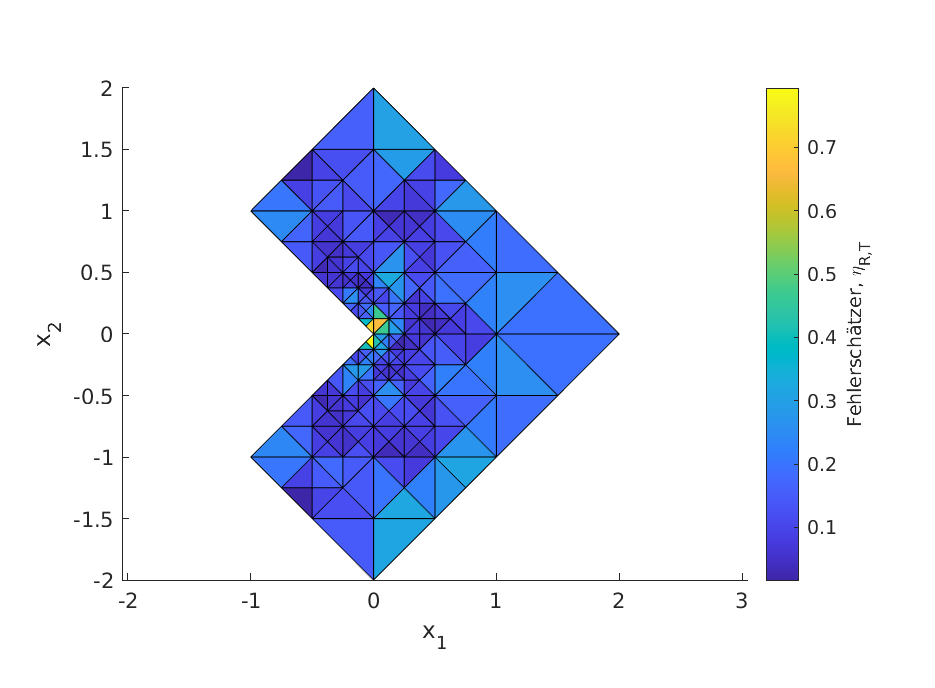
\includegraphics[width=\textwidth]{Plots/LShapeBenchmarkLocaletaR286}
\caption{lokaler Fehlerschätzer $\eta_{R,T}$}
\label{pl:LShapeLocaletaR286}
\end{subfigure}
\hfill
\begin{subfigure}[b]{0.45\textwidth}
\centering
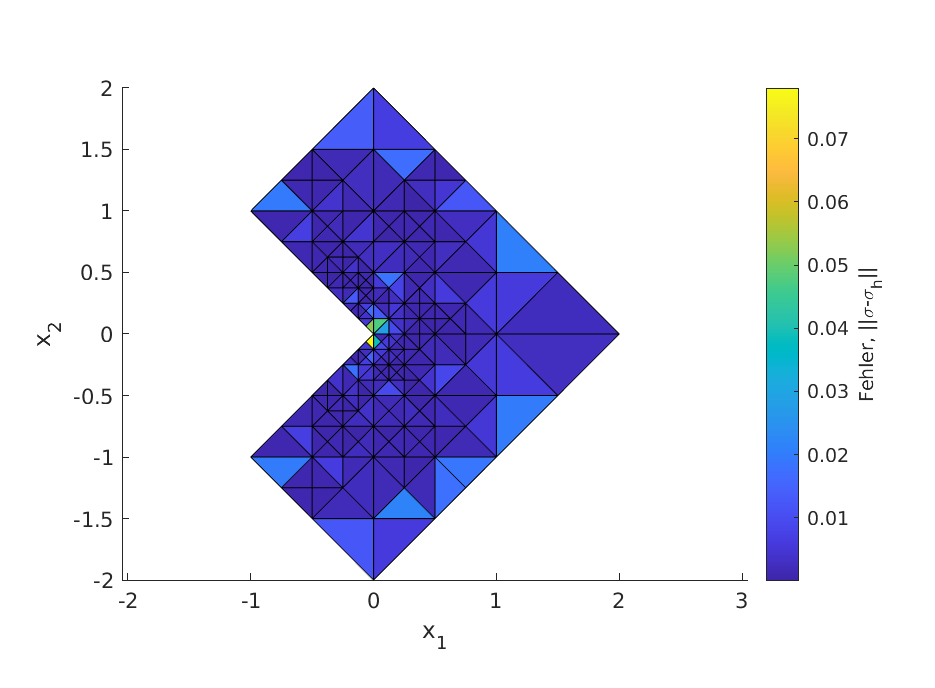
\includegraphics[width=\textwidth]{Plots/LShapeBenchmarkLocalNormSigDiff286}
\caption{lokaler Fehler $\norm{\sigma-\sigma_h}$}
\end{subfigure}
\caption{Adaptive Gitterverfeinerung mit dem residualen Fehlerschätzer $\eta_R$ und $d\cdot n=286$ Freiheitsgraden.}
\label{pl:LShapeLocalNormSigDiff286}
\end{figure}

\newpage
\subsection{Fazit}

Im ersten numerischen Experiment haben wir gesehen, dass die in Satz \ref{pr:APrioriFehler} a priori vorhergesagte lineare Konvergenz in der Praxis vom P1 Finiten Element erfüllt wird, sofern die Verschiebung $u$ regulär genug ist. Allerdings tritt unter anderem bei ungünstigen Materialparametern mit dieser Methode Locking auf. 

Die Konvergenz im zweiten Experiment mit uniformer Gitterverfeinerung ist aufgrund einer Singularität im Ursprung nicht mehr linear. Wir haben gesehen, dass adaptive Gitterverfeinerung mit dem Fehlerschätzer durch Mittelung hier keinen Mehrgewinn bringt, da dieser Fehlerschätzer nicht zuverlässig ist. Wir können dagegen mit der adaptiven Gitterverfeinerung mit dem residualen Fehlerschätzer die für das Verfahren optimale lineare Konvergenz zurückgewinnen. In beiden Experimenten wurde nochmal bestätigt, was im Abschnitt über den residualen Fehlerschätzer gezeigt wurde, nämlich, dass dieser zuverlässig und effizient ist.


\clearpage

%\section{Symbolverzeichnis, Literatur}
\addcontentsline{toc}{section}{\protect\numberline{}Symbolverzeichnis, Literatur}
\section*{Symbolverzeichnis}

\begin{tabular}{rl}
	$\Omega$ & eine Menge im $\R^d$ \\
	$\Gamma$ & Rand von $\Omega$ \\
	$\chi$ & Deformation \\
	$V$, $V^0$ & Mengen von Verschiebungen $H^1(\Omega;\R^{d\times d})$ und $\{v\in V\colon Mv = 0\}$ \\
	$u,v$ & Verschiebungen \\
	$f,g$ & Volumenkraftdichte und Oberflächenkraftdichte \\
	$M$ & Matrix für gleitende Randbedingungen, definiert auf Seite \pageref{ch:DefinitionM}  \\
	$\diver$ & Divergenz auf $H^1(\Omega;\R^d)$, definiert durch $\diver\sigma\coloneqq\sum_{j}\partial_j\sigma_{ij}e_i$ \\
	$\e$, $\sigma$ & linearisierter Verzerrungstensor und Spannungstensor \\
	$\gamma$, $\tau$ & Voigtrepresentation, definiert in \eqref{eq:DefinitionVoigtD2} und \eqref{eq:DefinitionVoigtD3} \\
	$\lambda,\mu,\nu$ & Lamé-Parameter und Poissonzahl \\
	$C$ & Hooke-Tensor, definiert in \eqref{eq:DefinitionHookeTensor} \\
	$a$ & Bilinearform, definiert in \eqref{eq:Definitiona} \\
	$\ell$ & Funktional, definiert in \eqref{eq:Definitionell} \\
	$W$ & Potenzielle Energie, definiert in \eqref{eq:DefinitionW} \\
	$H^k(\Omega)$, $H^k(\Omega;\R^d)$ & Sobolevräume $W^{k,p}(\Omega)$ und $W^{k,p}(\Omega;\R^d)$ mit $p=2$ \\
	$\inner{\cdot,\cdot}_{k,\Omega}$ & inneres Produkt auf $H^k(\Omega)$, $H^k(\Omega;\R^d)$ und $H^k(\Omega;\R^{d\times d})$ \\
	$\norm{\cdot}_{k,\Omega}$ & vom inneren Produkt induzierte Sobolevnorm \\
	$\abs{\cdot}_{1,\Omega}$ & Seminorm $\norm{\nabla\cdot}_{0,\Omega}$ \\
	$\norm{\cdot}_\infty$ & Supremumsnorm auf Sobolevräumen \\
	$\norm{\cdot}_F$ & Frobenius-Norm, induziert vom inneren Produkt "`$:$"' auf $\R^{d\times d}$  \\
	$\norm{\cdot}_K$ & Kornsche Norm, definiert in \eqref{eq:DefinitionKornNorm} \\
	$\epi$ & Epigraph einer Funktion \\
	$\psi$ & lokale Parametrisierung von $\Omega$ \\
	$A$ & affine Transformation oder Steifheitsmatrix \\
	$\theta$ & Abschneidefunktionen oder Zerlegung der Eins \\
	$\erw$ & Erweiterungsoperator \\
	$c_A$, $c_a$ & Stetigkeits- und Elliptizitätskonstante aus Propositionen \ref{pr:stetigkeita} und \ref{pr:elliptizitaeta} \\
	$c_c$ & Elliptizitätskonstante von $C$, definiert in \eqref{eq:HookeTensorEllipticity} \\
	$c_{E}$ & Stetigkeitskonstanten der Erweiterung $\erw$ aus Lemma \ref{le:ErweiterungVonEpigraphen} \\
	$c_{K1}$, $c_{K2}$ & Konstanten der Kornschen Ungleichungen aus Satz \ref{le:KornOhneRandbedingungen} und \ref{th:KornMitRandbedingungen} \\
	$c_{I1}$, $c_{I2}$ & Konstanten der Interpolationsoperatoren in Propositionen \ref{pr:Approximationssatz} und \ref{pr:ClementInterpolation} \\
	$\varphi,\phi$ & nodale Basis in einer und $d$ Dimensionen \\
	$V_h$, $V_h^0$ & P1-Finite-Elemente-Räume, definiert in Gleichungen \eqref{eq:definitionVh} und \eqref{eq:definitionVhHom} \\
	$u_h,v_h$ & Verschiebungen des diskreten Problems \\
	$\cT$ & zulässige Triangulierung \\
	$\cE$, $\cE_\Gamma$, $\cE_N$, $\cE_\Omega$ & Mengen von Kanten einer Triangulierung, definiert auf Seite \pageref{se:definitionEN} \\
	$\cN$, $\cN_\Gamma$ & Mengen von Knoten einer Triangulierung, definiert auf Seite \pageref{se:definitionEN} \\
	$h_T$, $h_E$ & Durchmesser $\diam(T)$ und Kantenlänge $\diam(E)$ \\
	$n$ & Anzahl der Knoten von $\cT$ oder äußere Normale \\
\end{tabular}

%Der Übersichtlichkeit halber werden bei Summen in dieser Arbeit meistens die Grenzen weggelassen. Die Menge der Indizes, über die sich die Summe erstreckt wird dann als maximal angenommen.


\begin{tabular}{rl}
	$e$ & Fehler $u-u_h$ oder Einheitsvektor $e_i=\delta_{\cdot i}$ \\
	$R_T$, $R_E$ & flächen- und kantenbezogene Residuen, definiert in \eqref{eq:DefinitionRT} und \eqref{eq:DefinitionRE} \\
%	$[\![\sigma n_E]\!]$ & Kantenbezogene Sprünge, definiert in \eqref{eq:DefinitionKantenbezSpruenge} \\
	$\eta_{R,T}$, $\eta_R$ & residualer Fehlerschätzer, definiert in \eqref{eq:DefinitionEtaRT} und \eqref{eq:DefinitionEtaR} \\
	$\eta_{M,T}$, $\eta_M$ & Fehlerschätzer durch Mittelung, definiert auf Seite \pageref{ch:DefinitionEtaM} \\
	$\tiomega_T$, $\omega_T$ & Umgebungen von $T$, definiert auf Seite \pageref{ch:DefinitionOmegaTildeT} und \pageref{ch:DefinitionOmegaT} \\
	$\omega_E$ & Umgebung von $E$, definiert auf Seite \pageref{ch:DefinitionOmegaT} \\
	$\omega_{x^i}$ & Umgebung von $x^i$, definiert auf Seite \pageref{ch:DefinitionEtaM} \\
\end{tabular}

\nocite{*}
\bibliographystyle{plain}
\bibliography{bibliographyFile}

%\begin{thebibliography}{00}
%
%\bibitem{Alt-2016}
%\newblock Alt, Hans Wilhelm.
%\newblock {\em Linear Functional Analysis: An Application-Oriented Introduction.}
%\newblock London: Springer London, 2016. 
%
%%\bibitem{Ban-2003}
%%\newblock Bangerth, Wolfgang, and Rolf Rannacher.
%%\newblock {\em Adaptive Finite Element Methods for Differential Equations.}
%%\newblock Basel [u.a.]: Birkhäuser, 2003. S.130f.
%
%\bibitem{Bra-2007}
%\newblock Braess, Dietrich.
%\newblock {\em Finite Elemente: Theorie, Schnelle Löser Und Anwendungen in Der Elastizitätstheorie.}
%\newblock 4., überarb. und erw. Aufl.
%\newblock Berlin [u.a.]: Springer, 2007.
%
%\bibitem{Car-2011}
%\newblock Carstensen, C., M. Eigel, and J. Gedicke.
%\newblock "`Computational Competition of Symmetric Mixed FEM in Linear Elasticity."'
%\newblock {\em Computer Methods in Applied Mechanics and Engineering 200}.41 (2011): 2903-2915.
%
%\bibitem{Cia-1988}
%\newblock Ciarlet, Philippe G.
%\newblock {\em Studies in Mathematics and Its Applications. Mathematical Elasticity. 1, Three-dimensional Elasticity.}
%\newblock Amsterdam [u.a.]: North-Holland, 1988.
%
%%\bibitem{Cia-1997}
%%\newblock Ciarlet, Philippe G.
%%\newblock {\em Studies in Mathematics and Its Applications. Mathematical Elasticity. 2, Theory of Plates.}
%%\newblock Amsterdam [u.a.]: North-Holland, 1997. 
%
%\bibitem{Con-2021}
%\newblock Conti, S.
%\newblock {\em Einführung in die Funktionanalysis.}
%\newblock Lecture notes. Universität Bonn, Wintersemester 2021/2022.
%
%\bibitem{Doe-1996}
%\newblock Dörfler, W.
%\newblock "`A Convergent Adaptive Algorithm for Poisson's Equation."' 
%\newblock {\em SIAM Journal On Numerical Analysis 33},
%\newblock no. 3 (1996): 1106-1124.
%
%\bibitem{Duv-1976}
%\newblock Lions, Jacques Louis, and Georges Duvaut.
%\newblock {\em Inequalities in Mechanics and Physics.}
%\newblock Berlin, Heidelberg: Springer, 1976. 
%
%\bibitem{Gei-2002}
%\newblock Geiger, Carl.
%\newblock {\em Theorie Und Numerik Restringierter Optimierungsaufgaben.}
%\newblock 1st ed. 2002. Berlin, Heidelberg: Springer Berlin Heidelberg, 2002.
%
%\bibitem{Ged-2021a}
%\newblock Gedicke, J.
%\newblock {\em Einführung in die Numerische Mathematik.}
%\newblock Lecture notes. Universität Bonn, Sommersemester 2021.
%
%\bibitem{Ged-2021b}
%\newblock Gedicke, J.
%\newblock {\em Wissenschaftliches Rechnen I.}
%\newblock Lecture notes. Universität Bonn, Wintersemester 2021/2022.
%
%\bibitem{Hod-1961}
%\newblock Hodge, PG.
%\newblock "`On Isotropic Cartesian Tensors."'
%\newblock {\em The American Mathematical Monthly 68}, no. 8 (1961): 793-795.
%
%\bibitem{Kik-1988}
%\newblock Kikuchi, Noboru, and John Tinsley Oden.
%\newblock {\em Contact Problems in Elasticity: A Study of Variational Inequalities and Finite Element Methods.}
%\newblock Philadelphia: SIAM, 1988. 
%
%%\bibitem{Kur-1994}
%%\newblock Kurt, Georg, and Johannes Tausch
%%\newblock "Some Error Estimates for the Numerical Approximation of Surface Integrals"
%%\newblock {\em Mathemtics of Computation 62}, no 206 (1994): 755-763.
%%\newblock https://www.ams.org/journals/mcom/1994-62-206/S0025-5718-1994-1219704-1/S0025-5718-1994-1219704-1.pdf
%
%\bibitem{Lif-1959}
%\newblock Lifshitz, Evgenii Mikhailovich, and Lev Davidovich Landau.
%\newblock {\em Course of Theoretical Physics.}
%\newblock Pergamon, 1959.
%
%\bibitem{Mar-2003}
%\newblock Martinec, Z.
%\newblock {\em Continuum Mechanics.}
%\newblock Lecture notes. Charles University, Prague. Jan 11, 2011.
%
%%\bibitem{Nei-2004}
%%\newblock Neittaanmäki, Pekka, and Sergey R. Repin.
%%\newblock {\em Reliable Methods for Computer Simulation: Error Control and Posteriori Estimates}.
%%\newblock Oxford: Elsevier Science \& Technology, 2004.
%
%\bibitem{Nit-1981}
%\newblock Nitsche, J. A.
%\newblock {\em On Korn's second inequality.}
%\newblock RAIRO Anal. Numér.  15  (1981),  no. 3, 237--248.
%
%\bibitem{Ver-2013}
%\newblock Verfürth, Rüdiger.
%\newblock {\em A Posteriori Error Estimation Techniques for Finite Element Methods.}
%\newblock Oxford: Oxford Univ. Press, 2013. 
%\end{thebibliography}

\end{document}
